\documentclass{report}

% simple paragraph stuff
\parindent=0pt
\parskip=6pt

% include \paragraph as numbered
\setcounter{secnumdepth}{3}
\setcounter{tocdepth}{3}

\usepackage[bookmarks=true]{hyperref}

% symbols
\usepackage{amsmath} % assumes amsmath package installed
\usepackage{amssymb} % for \square

% from http://tex.stackexchange.com/a/5255
\DeclareMathOperator*{\argmin}{arg\,min}

% algorithm stuff
\usepackage{algorithm}
\usepackage[noend]{algpseudocode}

% theorems
\newtheorem{invariant}{Invariant}
\newtheorem{theorem}{Theorem}
\newtheorem{proposition}{Proposition}
\newtheorem{lemma}{Lemma}
% from http://www.maths.tcd.ie/~dwilkins/LaTeXPrimer/Theorems.html
\newenvironment{proof}[1][Proof]{\begin{trivlist}
   \item[\hskip \labelsep {\bfseries #1}]}{\hfill$\square$\end{trivlist}}

\usepackage{array}
\usepackage{graphicx}
\usepackage{subcaption}

\usepackage{tikz}
\usetikzlibrary{arrows,backgrounds,calc,positioning,shapes,decorations.pathmorphing}

% plots
\usepackage{pgfplots}

% tables
\usepackage{multirow}
\usepackage{booktabs}

\usepackage{titling}

\usepackage{changepage} % for adjustwidth

%\def\hidenotes{}
% list of commenters
\newcommand{\ssnote}[1]{{\xxnote{SS}{red}{#1}}}
\newcommand{\cdnote}[1]{{\xxnote{CD}{blue}{#1}}}
\newcommand{\mknote}[1]{{\xxnote{MK}{green}{#1}}}
% implement conditional notes (turn on/off with \hidenotes above)
\newcommand{\xxnote}[3]{}
\ifx\hidenotes\undefined
  \usepackage{color}
  \renewcommand{\xxnote}[3]{\color{#2}{#1: #3}}
\fi

% wide page for side by side figures, tables, etc
% see http://tex.stackexchange.com/a/154766
\newlength{\offsetpage}
\setlength{\offsetpage}{1.5in}
\newenvironment{widepage}
   {\begin{adjustwidth}{-\offsetpage}{-\offsetpage}%
    \addtolength{\textwidth}{2\offsetpage}}%
{\end{adjustwidth}}

\title{Fast Manipulation\\Task Planning}
\author{Christopher M. Dellin}
\date{\today}

\renewcommand{\maketitlehookd}{
\begin{center}
\vspace{0.7in}
The Robotics Institute\\
Carnegie Mellon University\\
Pittsburgh, PA 15213\\
\vspace{0.7in}
\textbf{Thesis Committee:}\\
Siddhartha Srinivasa, CMU RI (Chair)\\
Anthony Stentz, CMU RI\\
Maxim Likhachev, CMU RI\\
Lydia Kavraki, Rice University\\
%\vspace{0.7in}
%\emph{Submitted in partial fulfillment of the requirements\\
%for the degree of Doctor of Philosophy.}
\end{center}
}

\begin{document}

\maketitle

\begin{abstract}
Driven by a symbolic task planner, plan a feasible or low-cost sequence of
robot trajectory segments to solve a multi-step manipulation problem
(e.g. move an object, turn a valve, etc).

\textbf{From RSS paper:}
Motion planning approaches that build graphs
in the collision-free subset of configuration space
have proven promising
for high-dimensional articulated robotics problems
in unstructured environments.
However, many complex tasks (e.g. manipulation)
present two primary challenges.
First, the subset of collision-free configurations changes each time
the robot, objects, or people move, items are grasped or released,
or the fidelity of the robot's models changes.
This makes it difficult not only to apply the results of prior
planning computation to the current problem,
but also to efficiently consider planned or hypothesized motions,
especially in multi-step tasks.
Second, human-scale tasks are time-sensitive,
and these approaches incur significant planning cost
(comparable to execution cost)
which is dominated by collision checking.
To address these challenges,
we make two principal contributions.
First, we introduce \emph{multi-set planning},
a formulation which explicitly represents structure
between similar problems in C-space
using set-theoretic relations
and a cost model incorporating both planning and execution costs.
Second, we present the \emph{Multi-Set PRM} algorithm
which exploits this representation
by applying best-first search over roadmaps
with an objective which optimistically minimizes these costs.
We show that this approach automatically reuses planning computation
from similar problems when useful,
naturally replicating diverse behavior from prior
manipulation work designed to improve planner efficiency,
such as cached graphs, conservative bounding volumes,
and handling of dynamic environments.
We detail experimental results on a multi-step
manipulation task which show greater than a 3x improvement
in planning costs,
and provide an open-source implementation of our planner.
\end{abstract}

\tableofcontents


%\begin{figure}
%\begin{widepage}
%   \centering
%   \begin{subfigure}[b]{0.24\textwidth}
%      \begin{center}
%      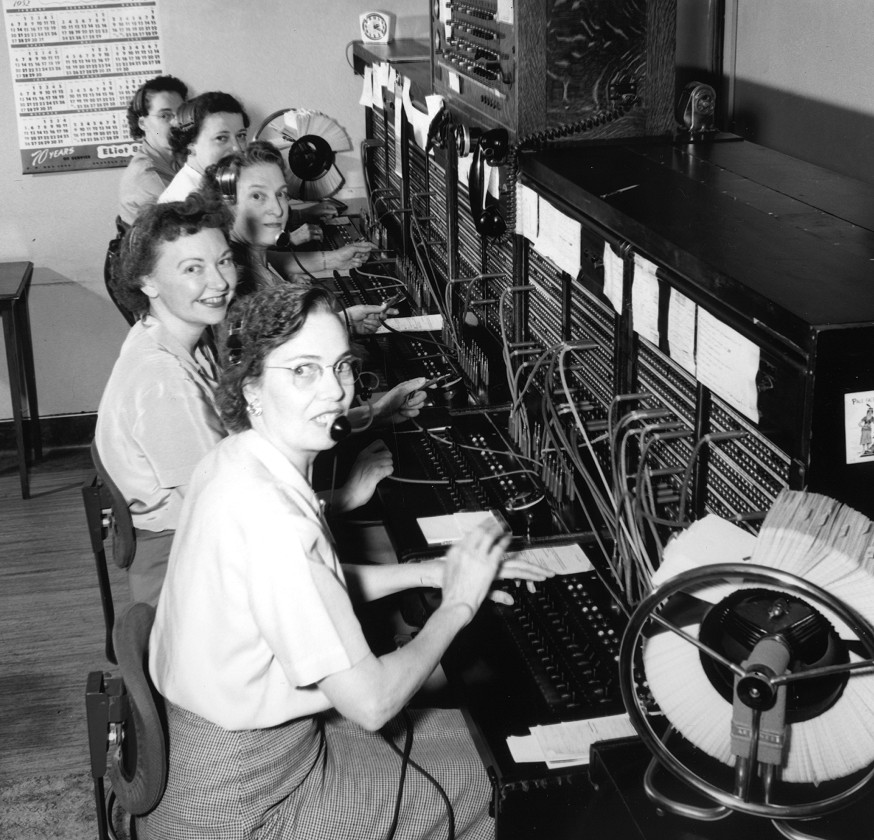
\includegraphics[width=\textwidth]{figs/switchboard.jpg}
%      
%      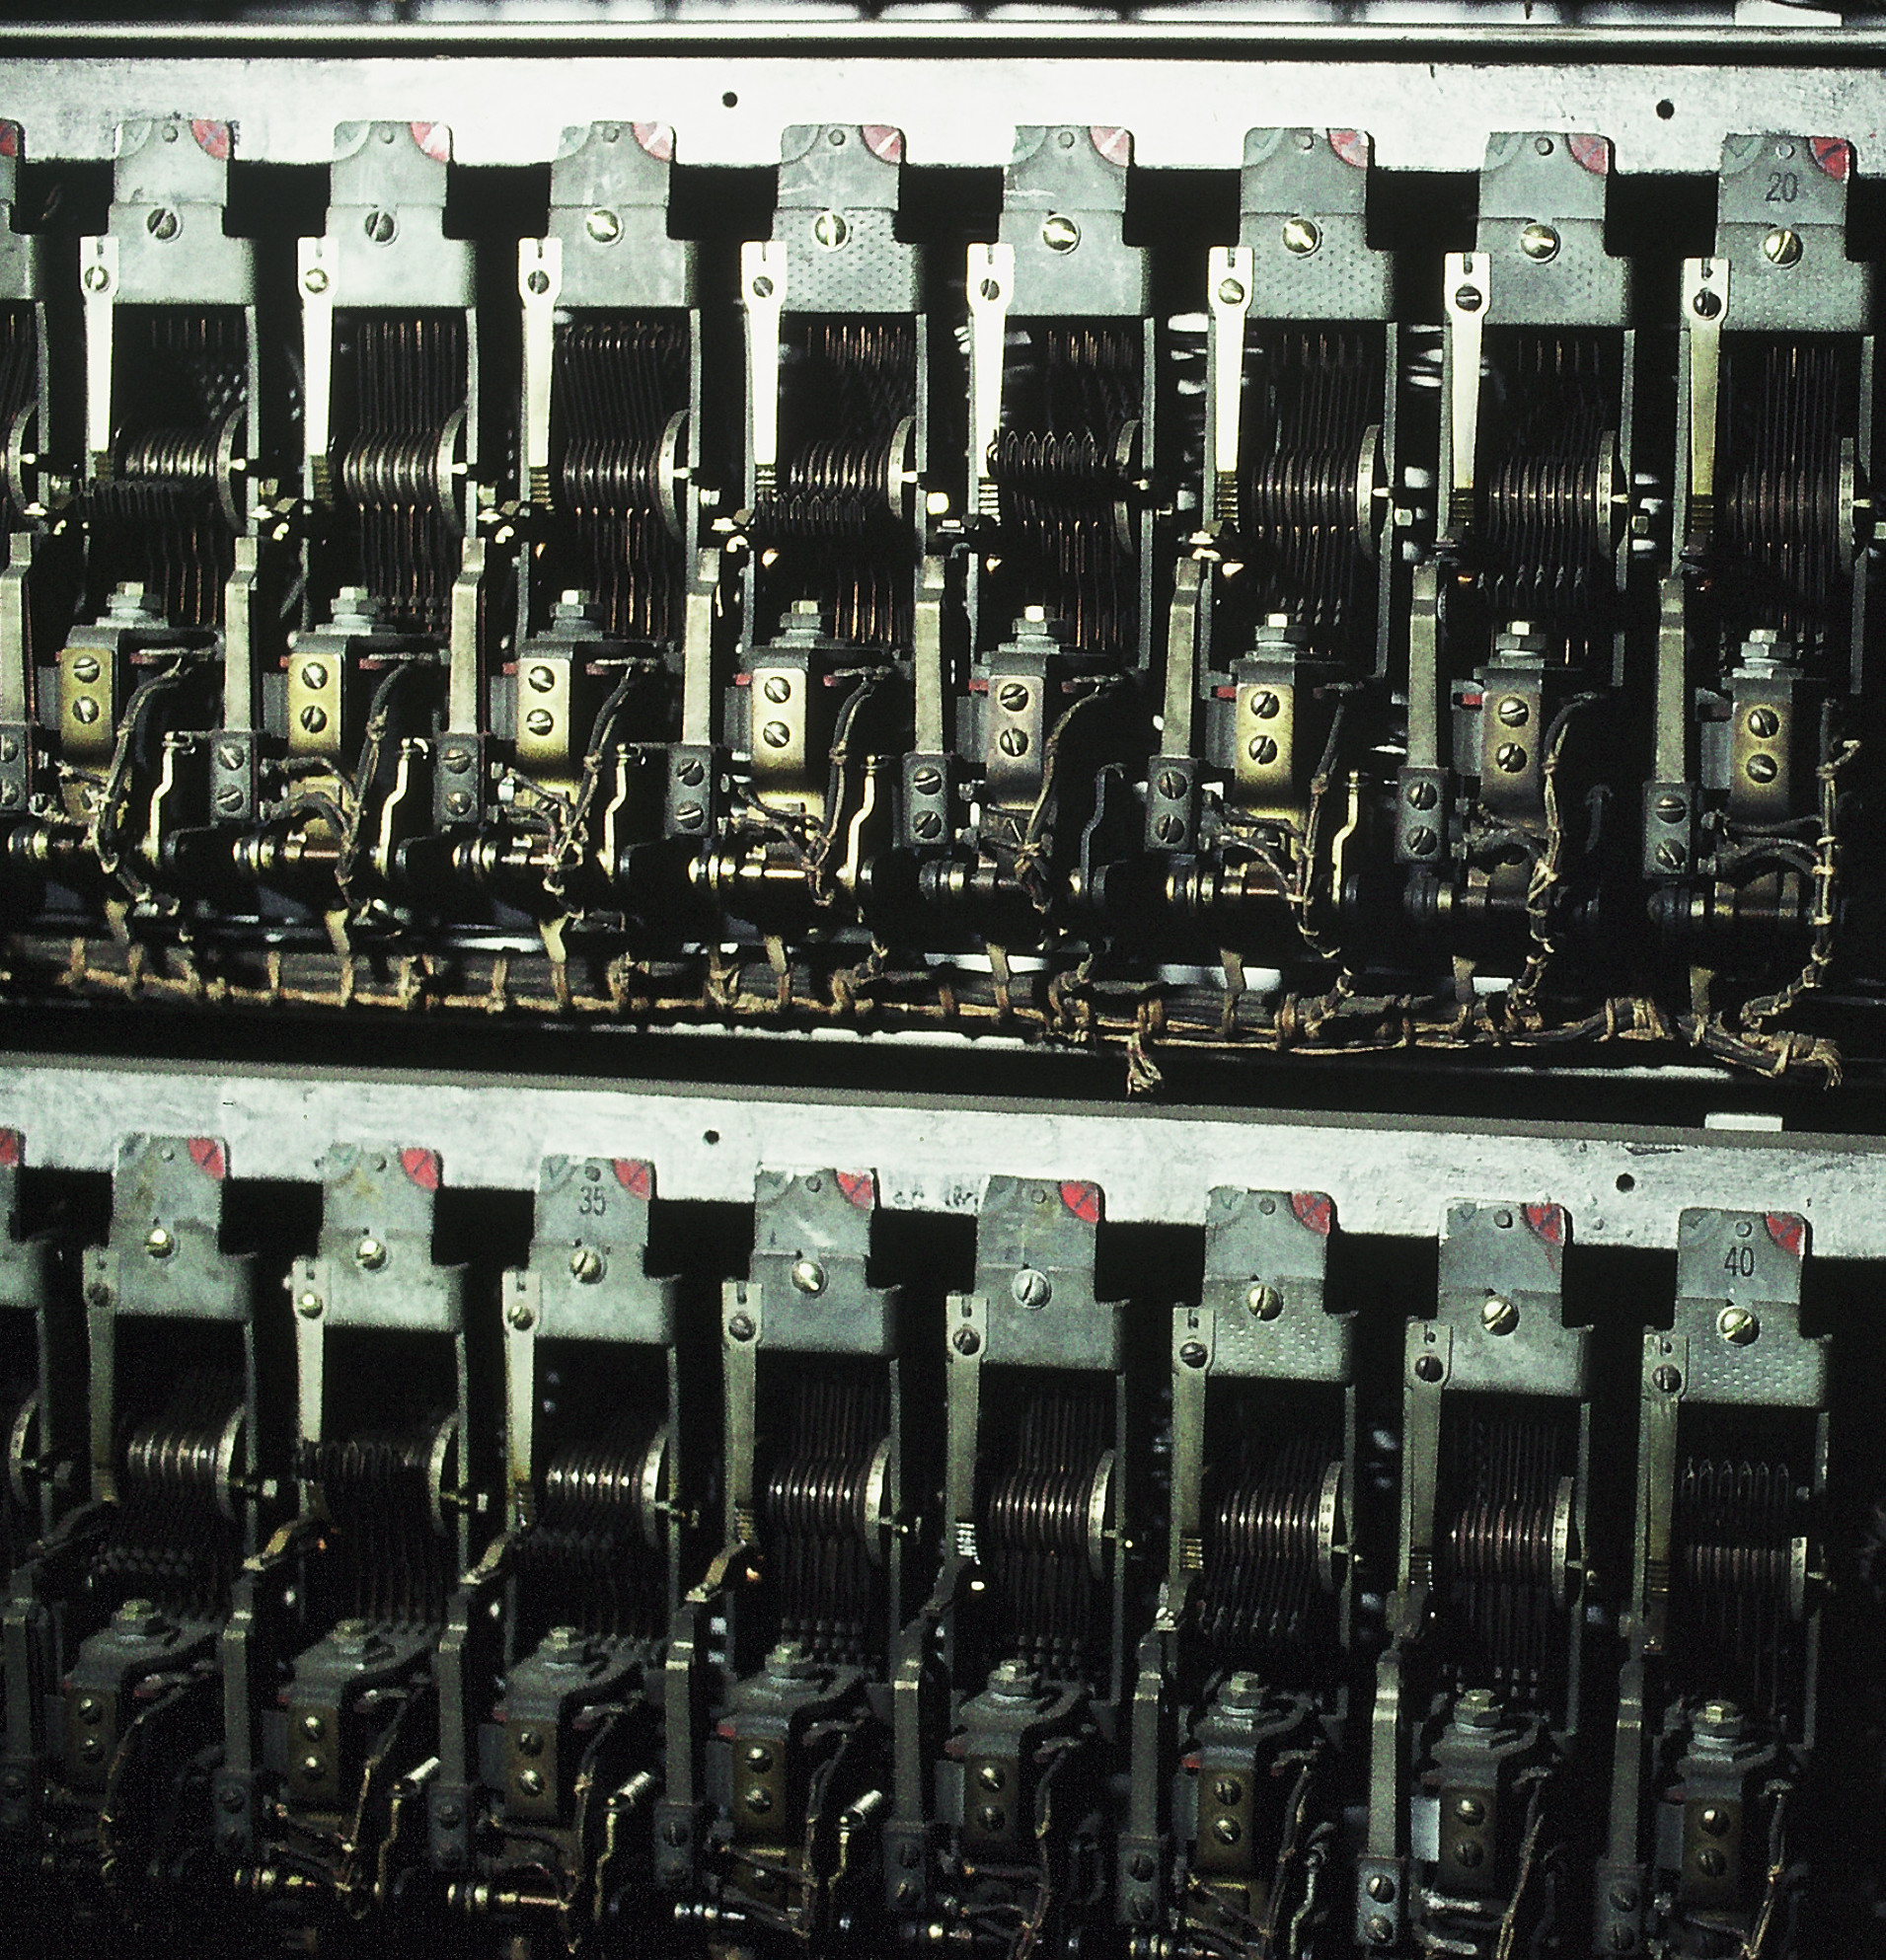
\includegraphics[width=\textwidth]{figs/mech-switches.jpg}
%      \end{center}
%      \caption{Something}
%   \end{subfigure}
%   \begin{subfigure}[b]{0.24\textwidth}
%      \begin{center}
%      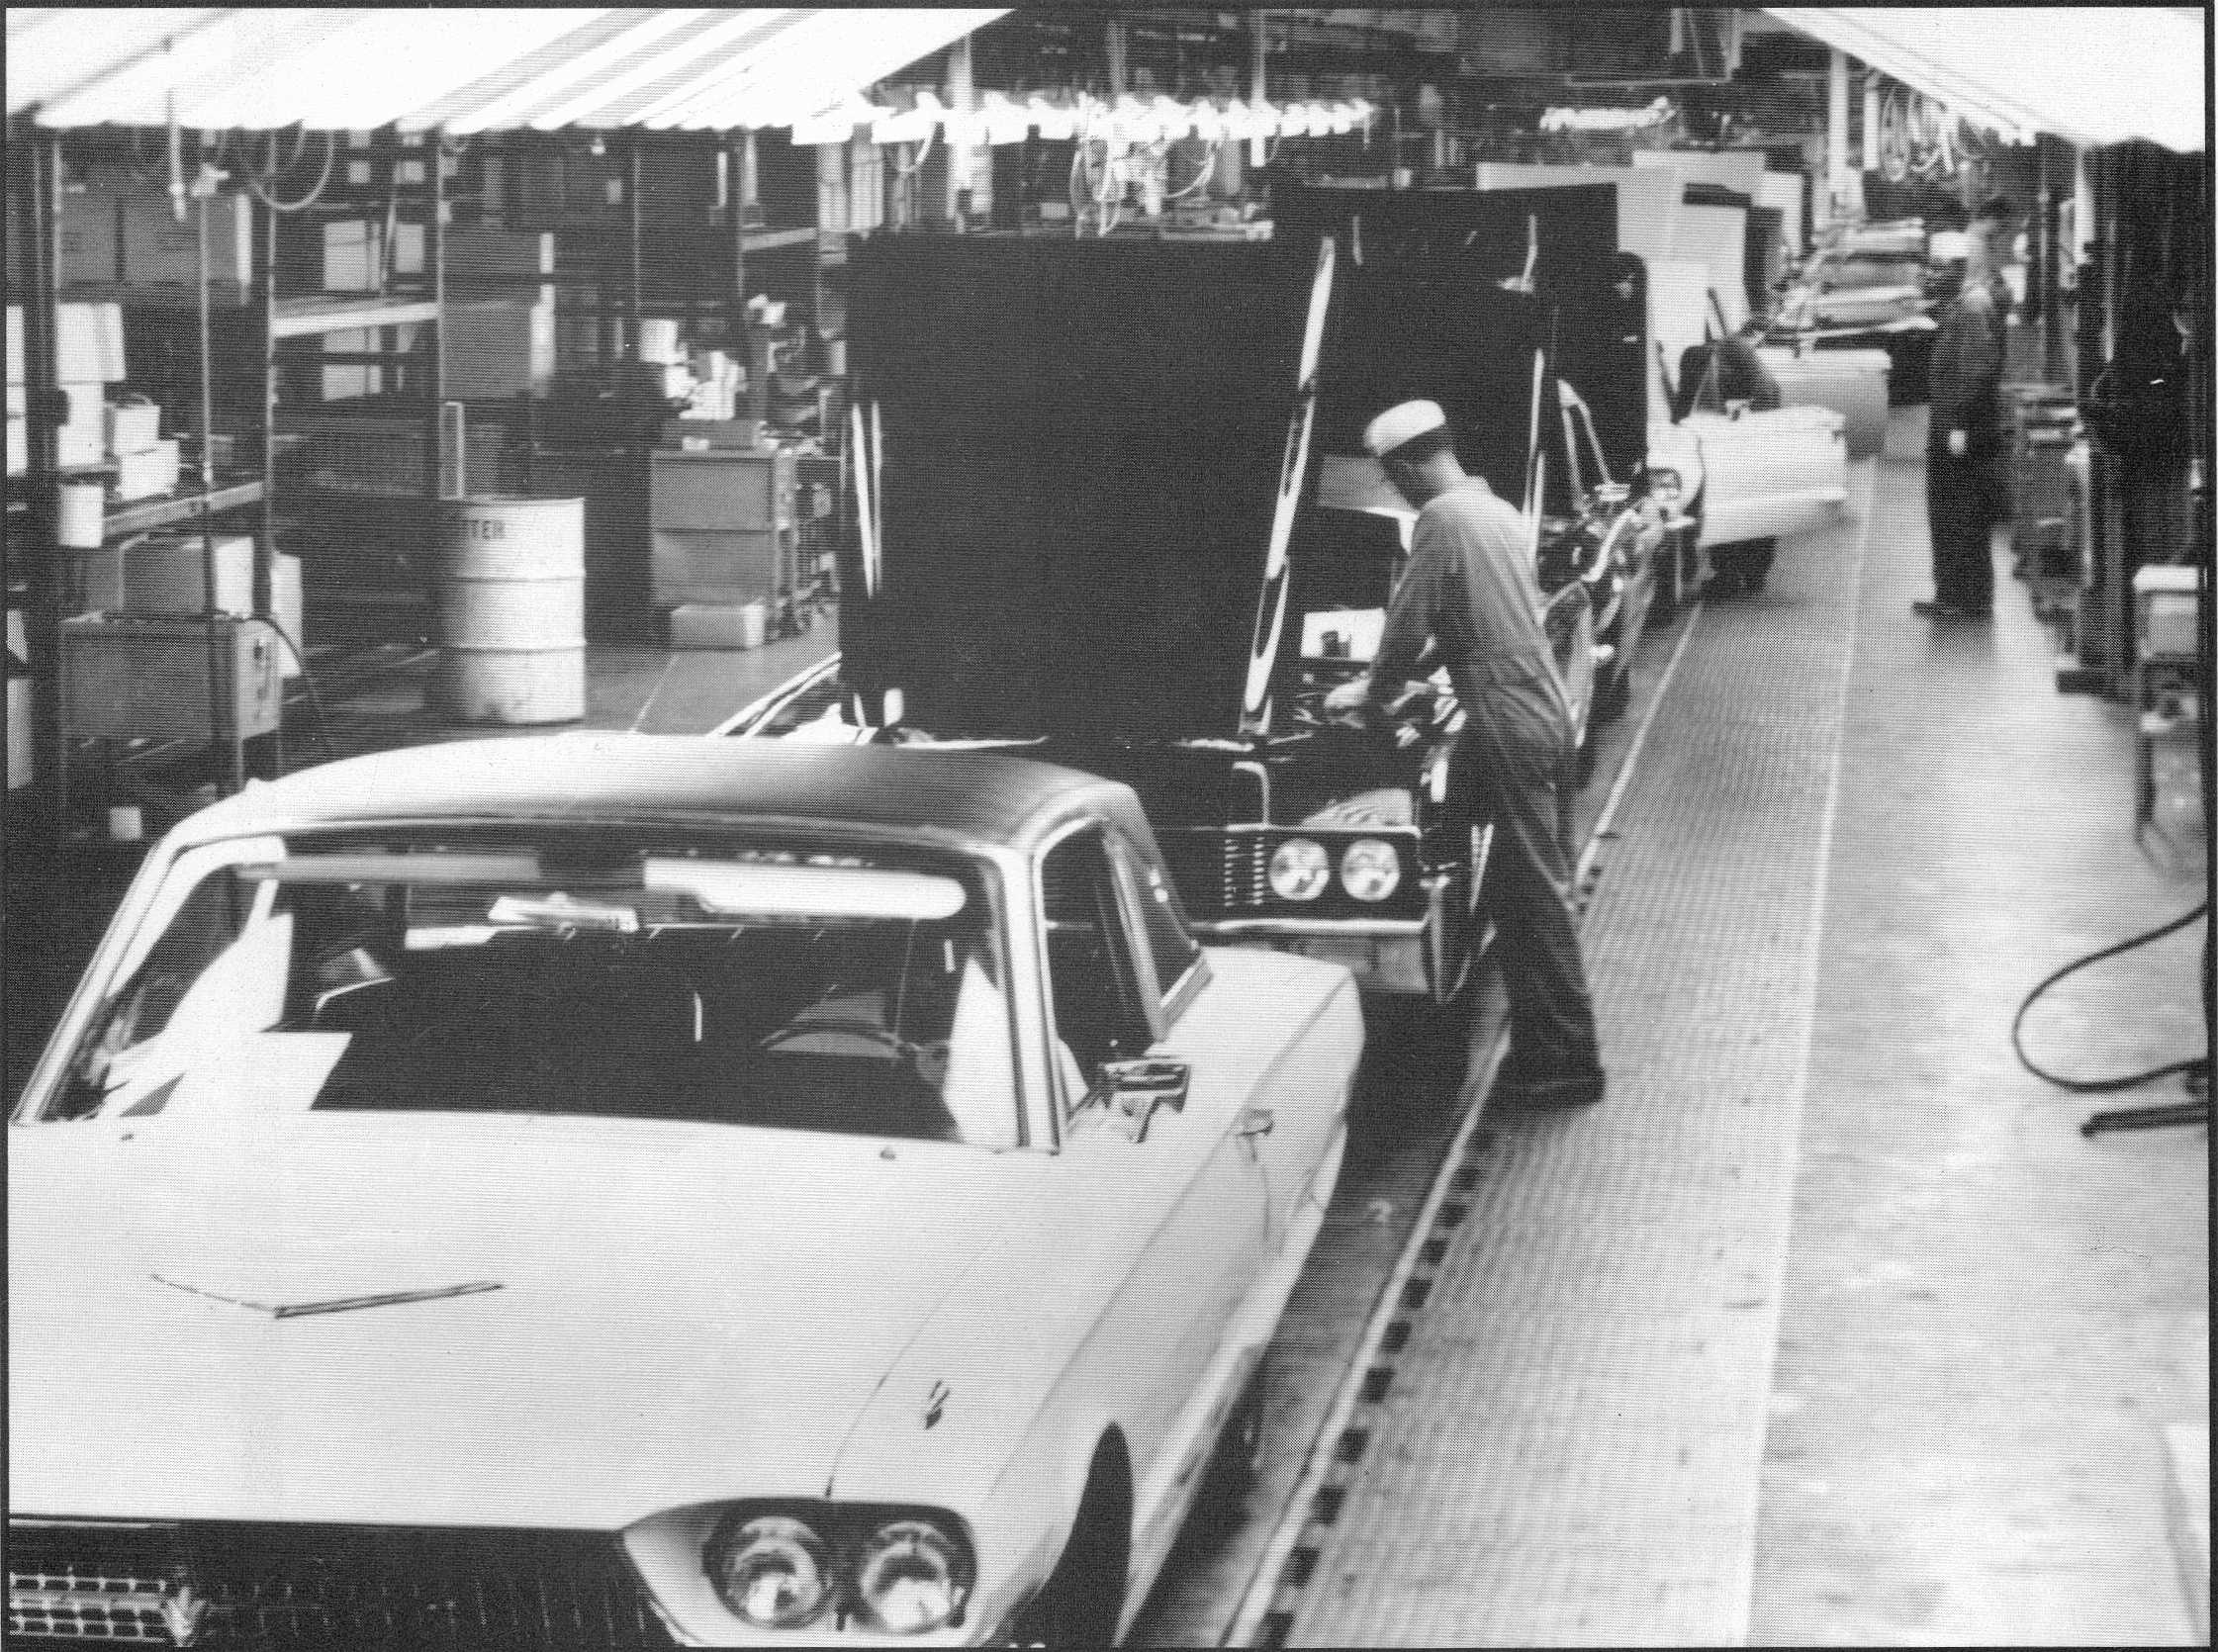
\includegraphics[width=\textwidth]{figs/assembly-line.jpg}
%      
%      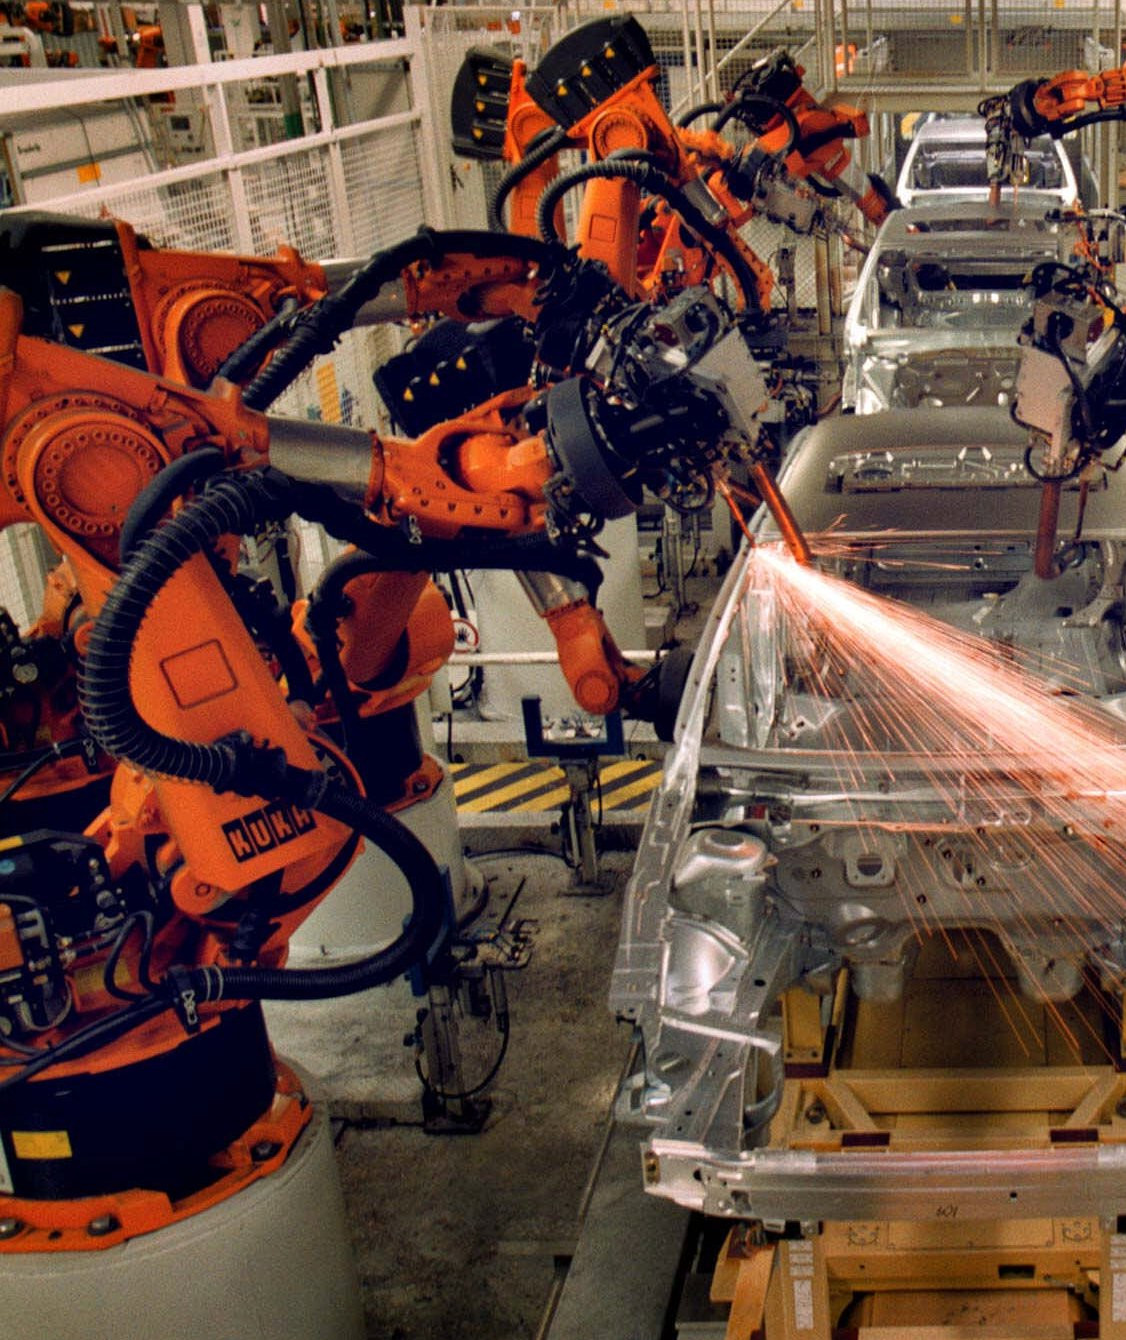
\includegraphics[width=\textwidth]{figs/car-robots.jpg}
%      \end{center}
%      \caption{Something}
%   \end{subfigure}
%   \begin{subfigure}[b]{0.24\textwidth}
%      \begin{center}
%      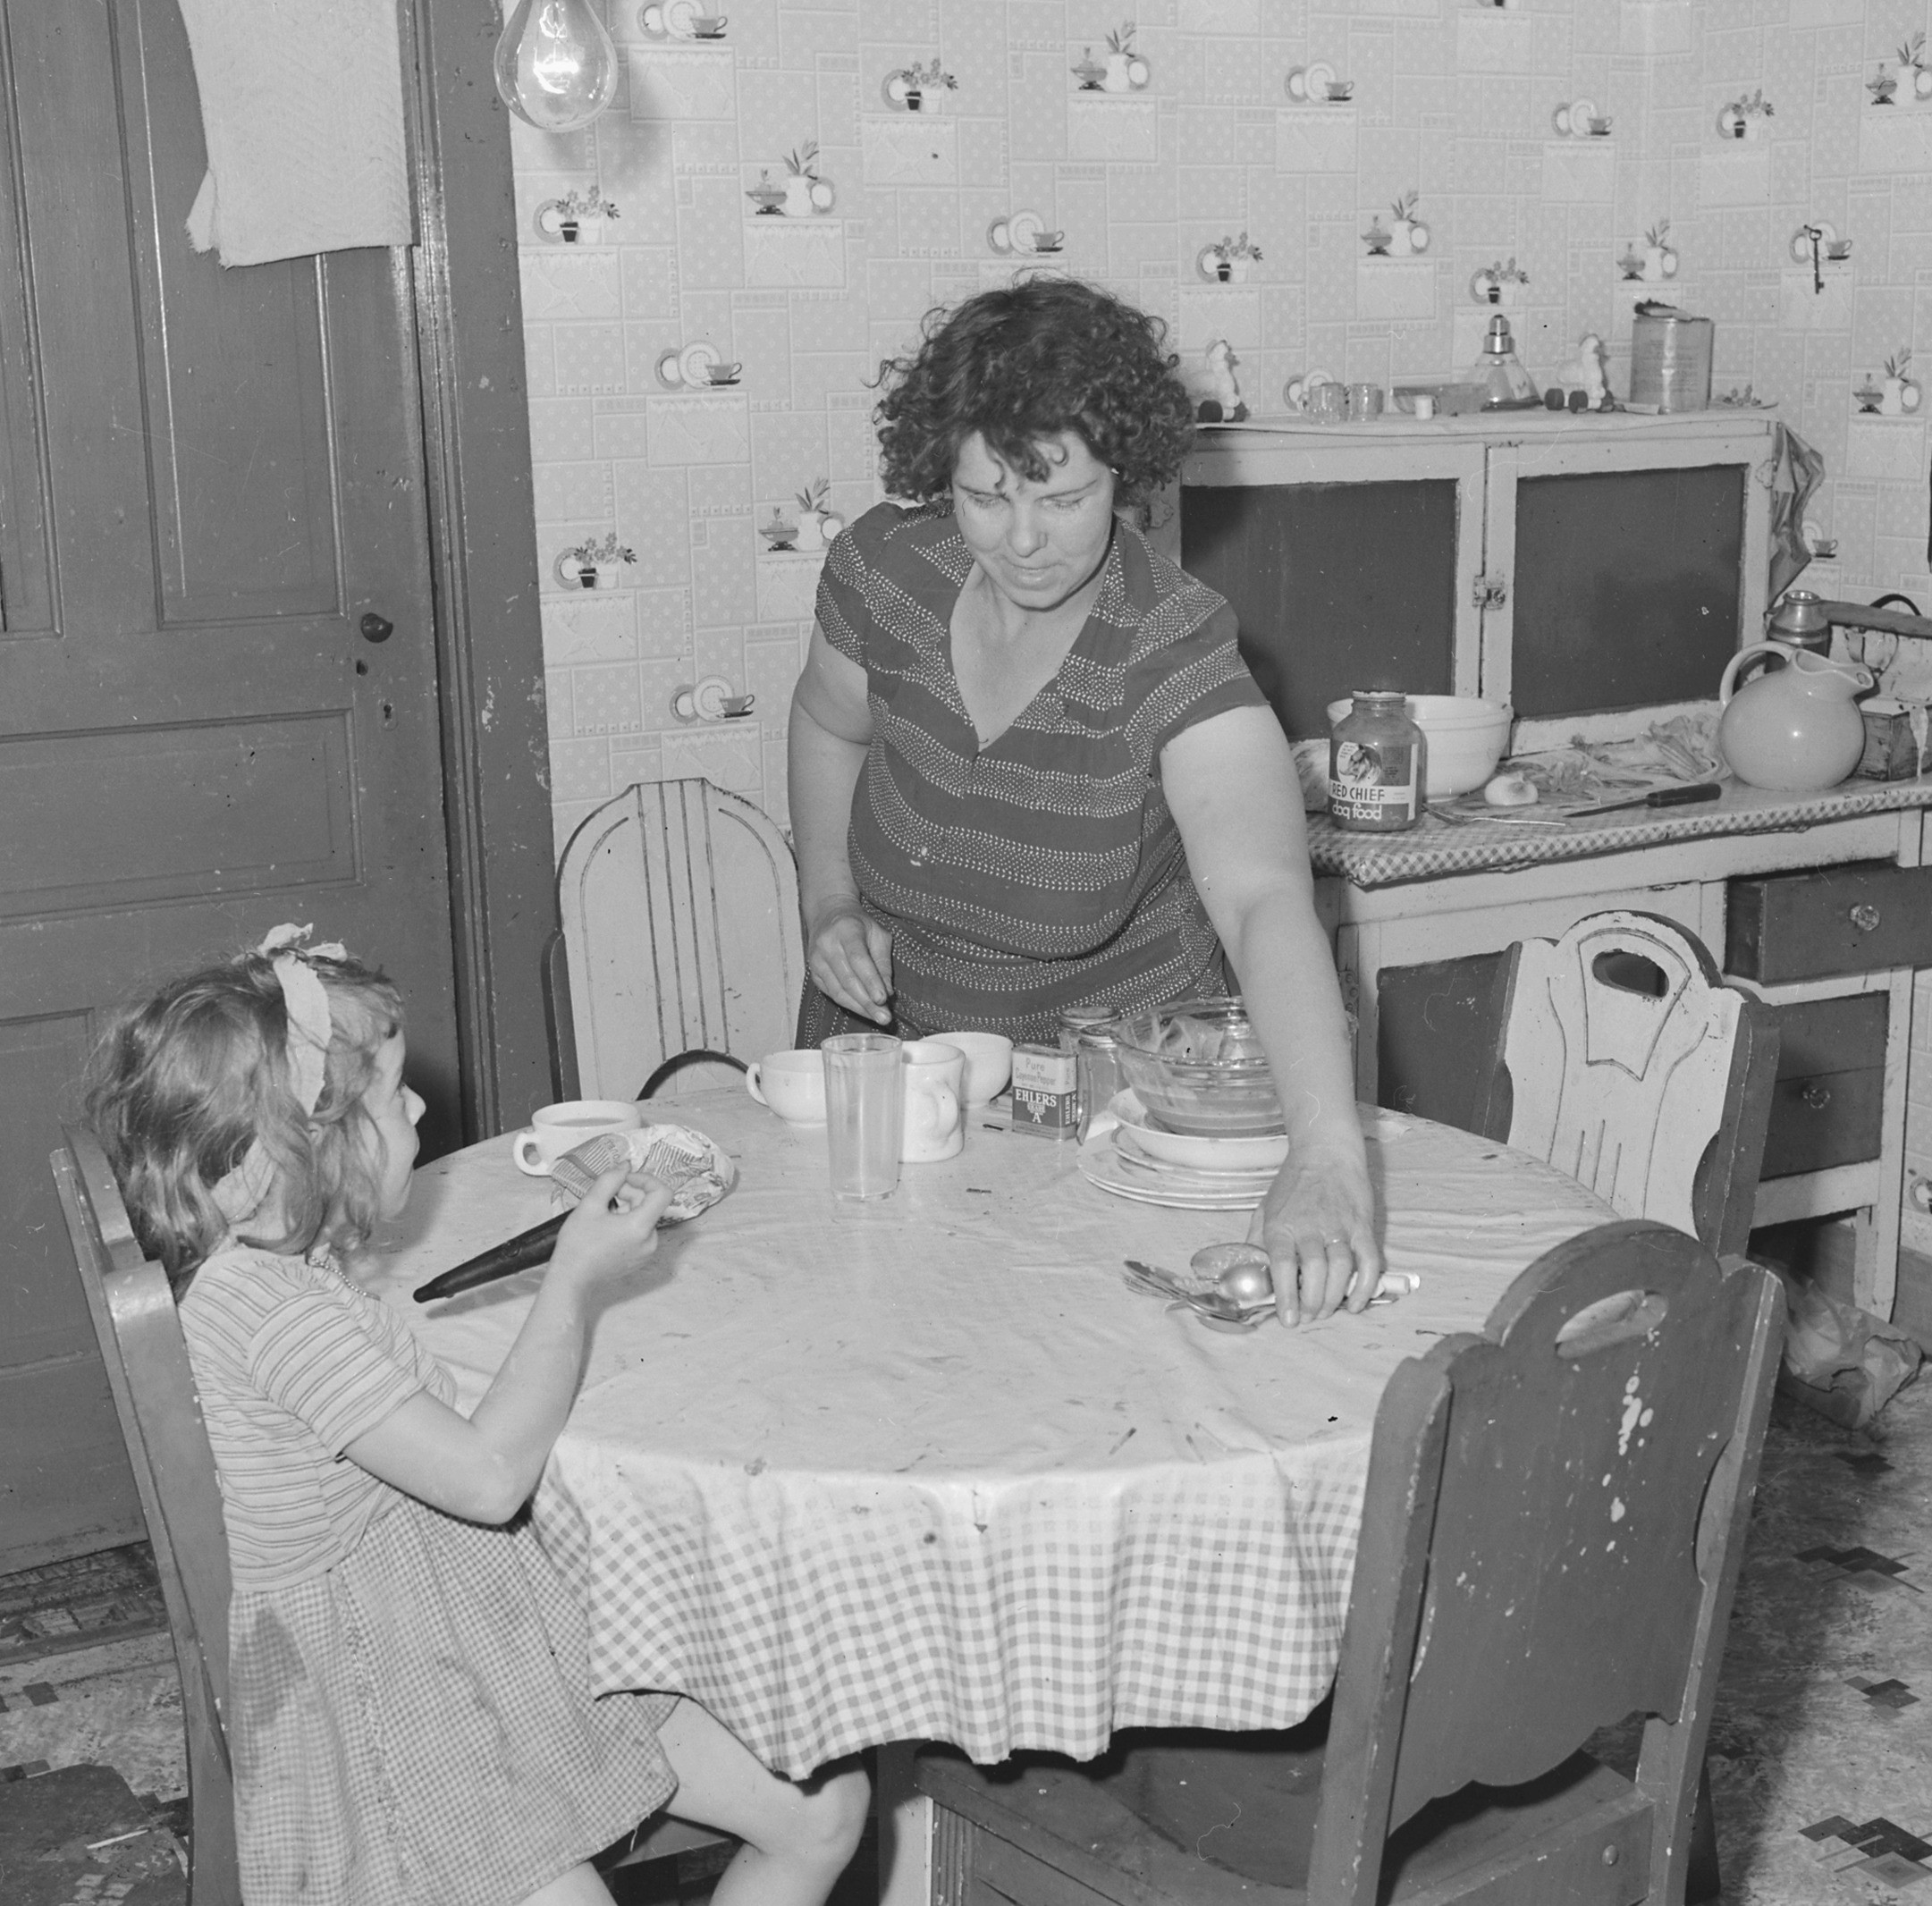
\includegraphics[width=\textwidth]{figs/table-clearing.jpg}
%      
%      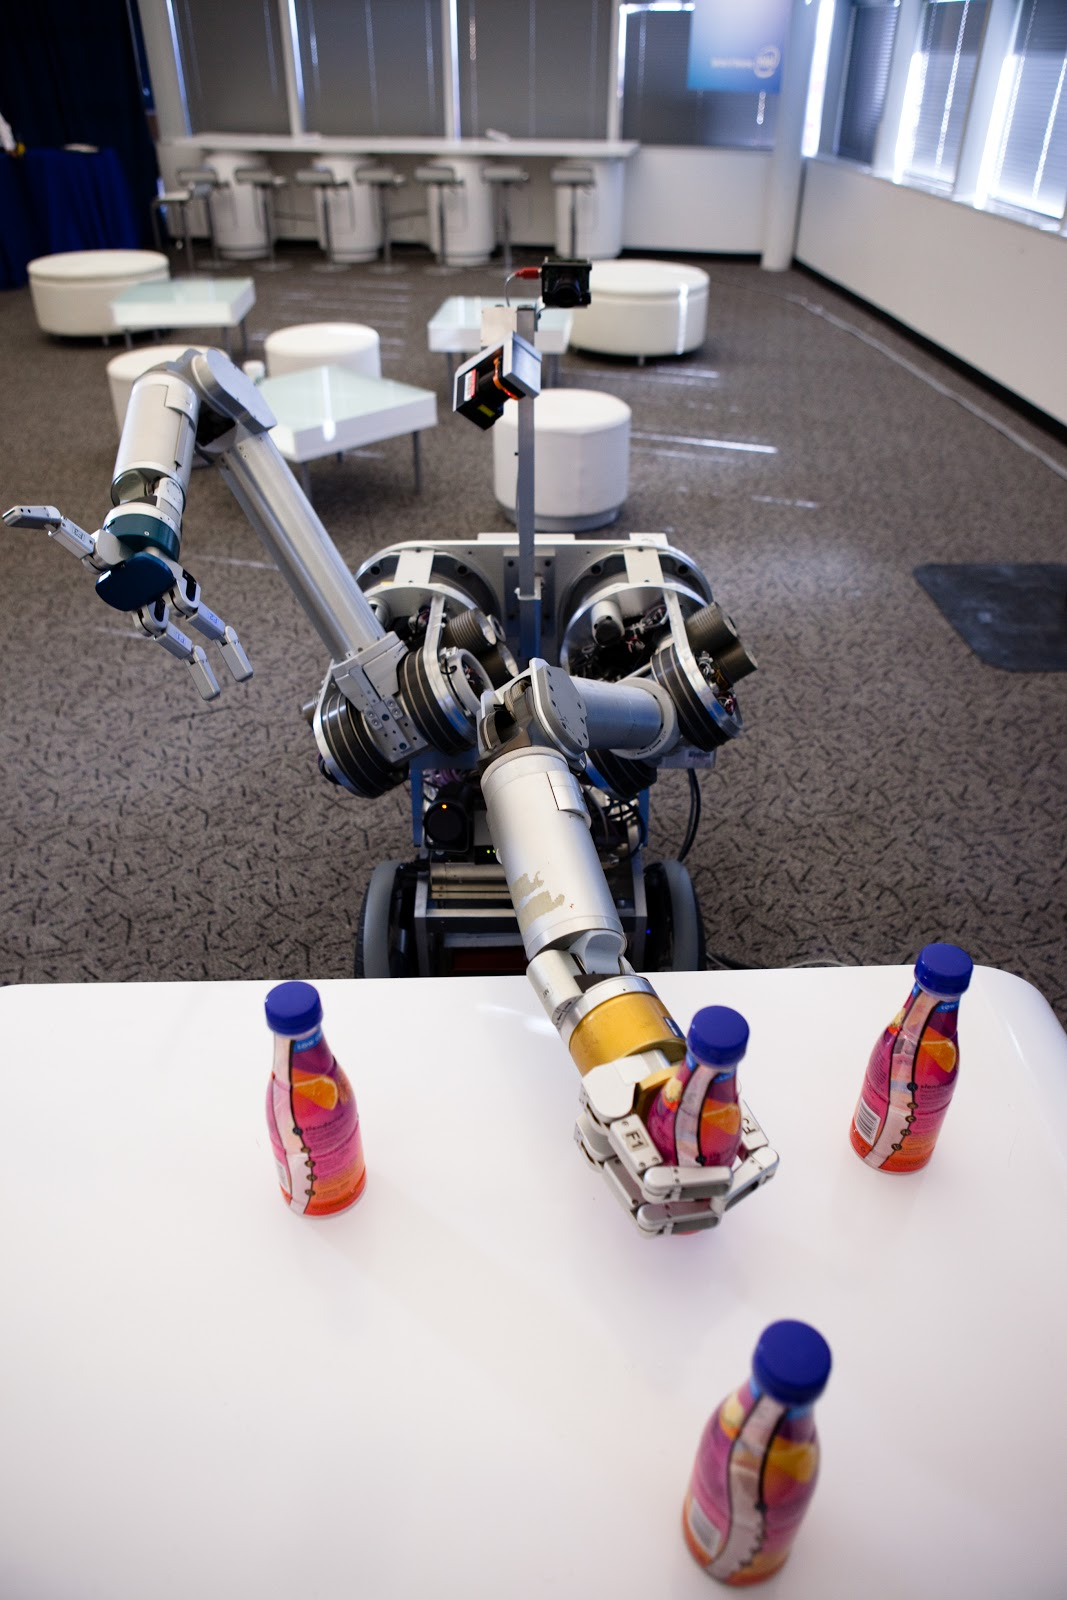
\includegraphics[height=2in]{figs/herb-fuze.jpg}
%      \end{center}
%      \caption{HERB Robot}
%   \end{subfigure}
%   \begin{subfigure}[b]{0.24\textwidth}
%      \begin{center}
%      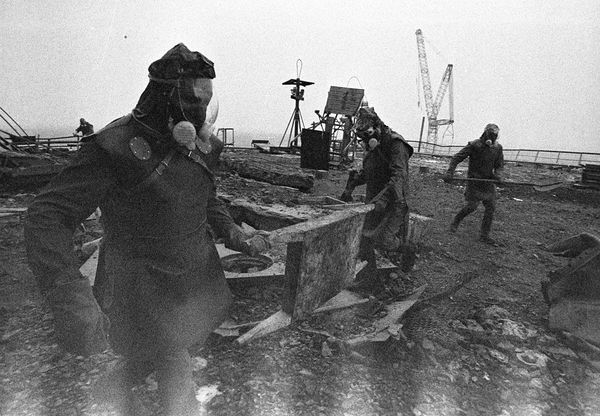
\includegraphics[width=\textwidth]{figs/chernobyl.jpg}
%      
%      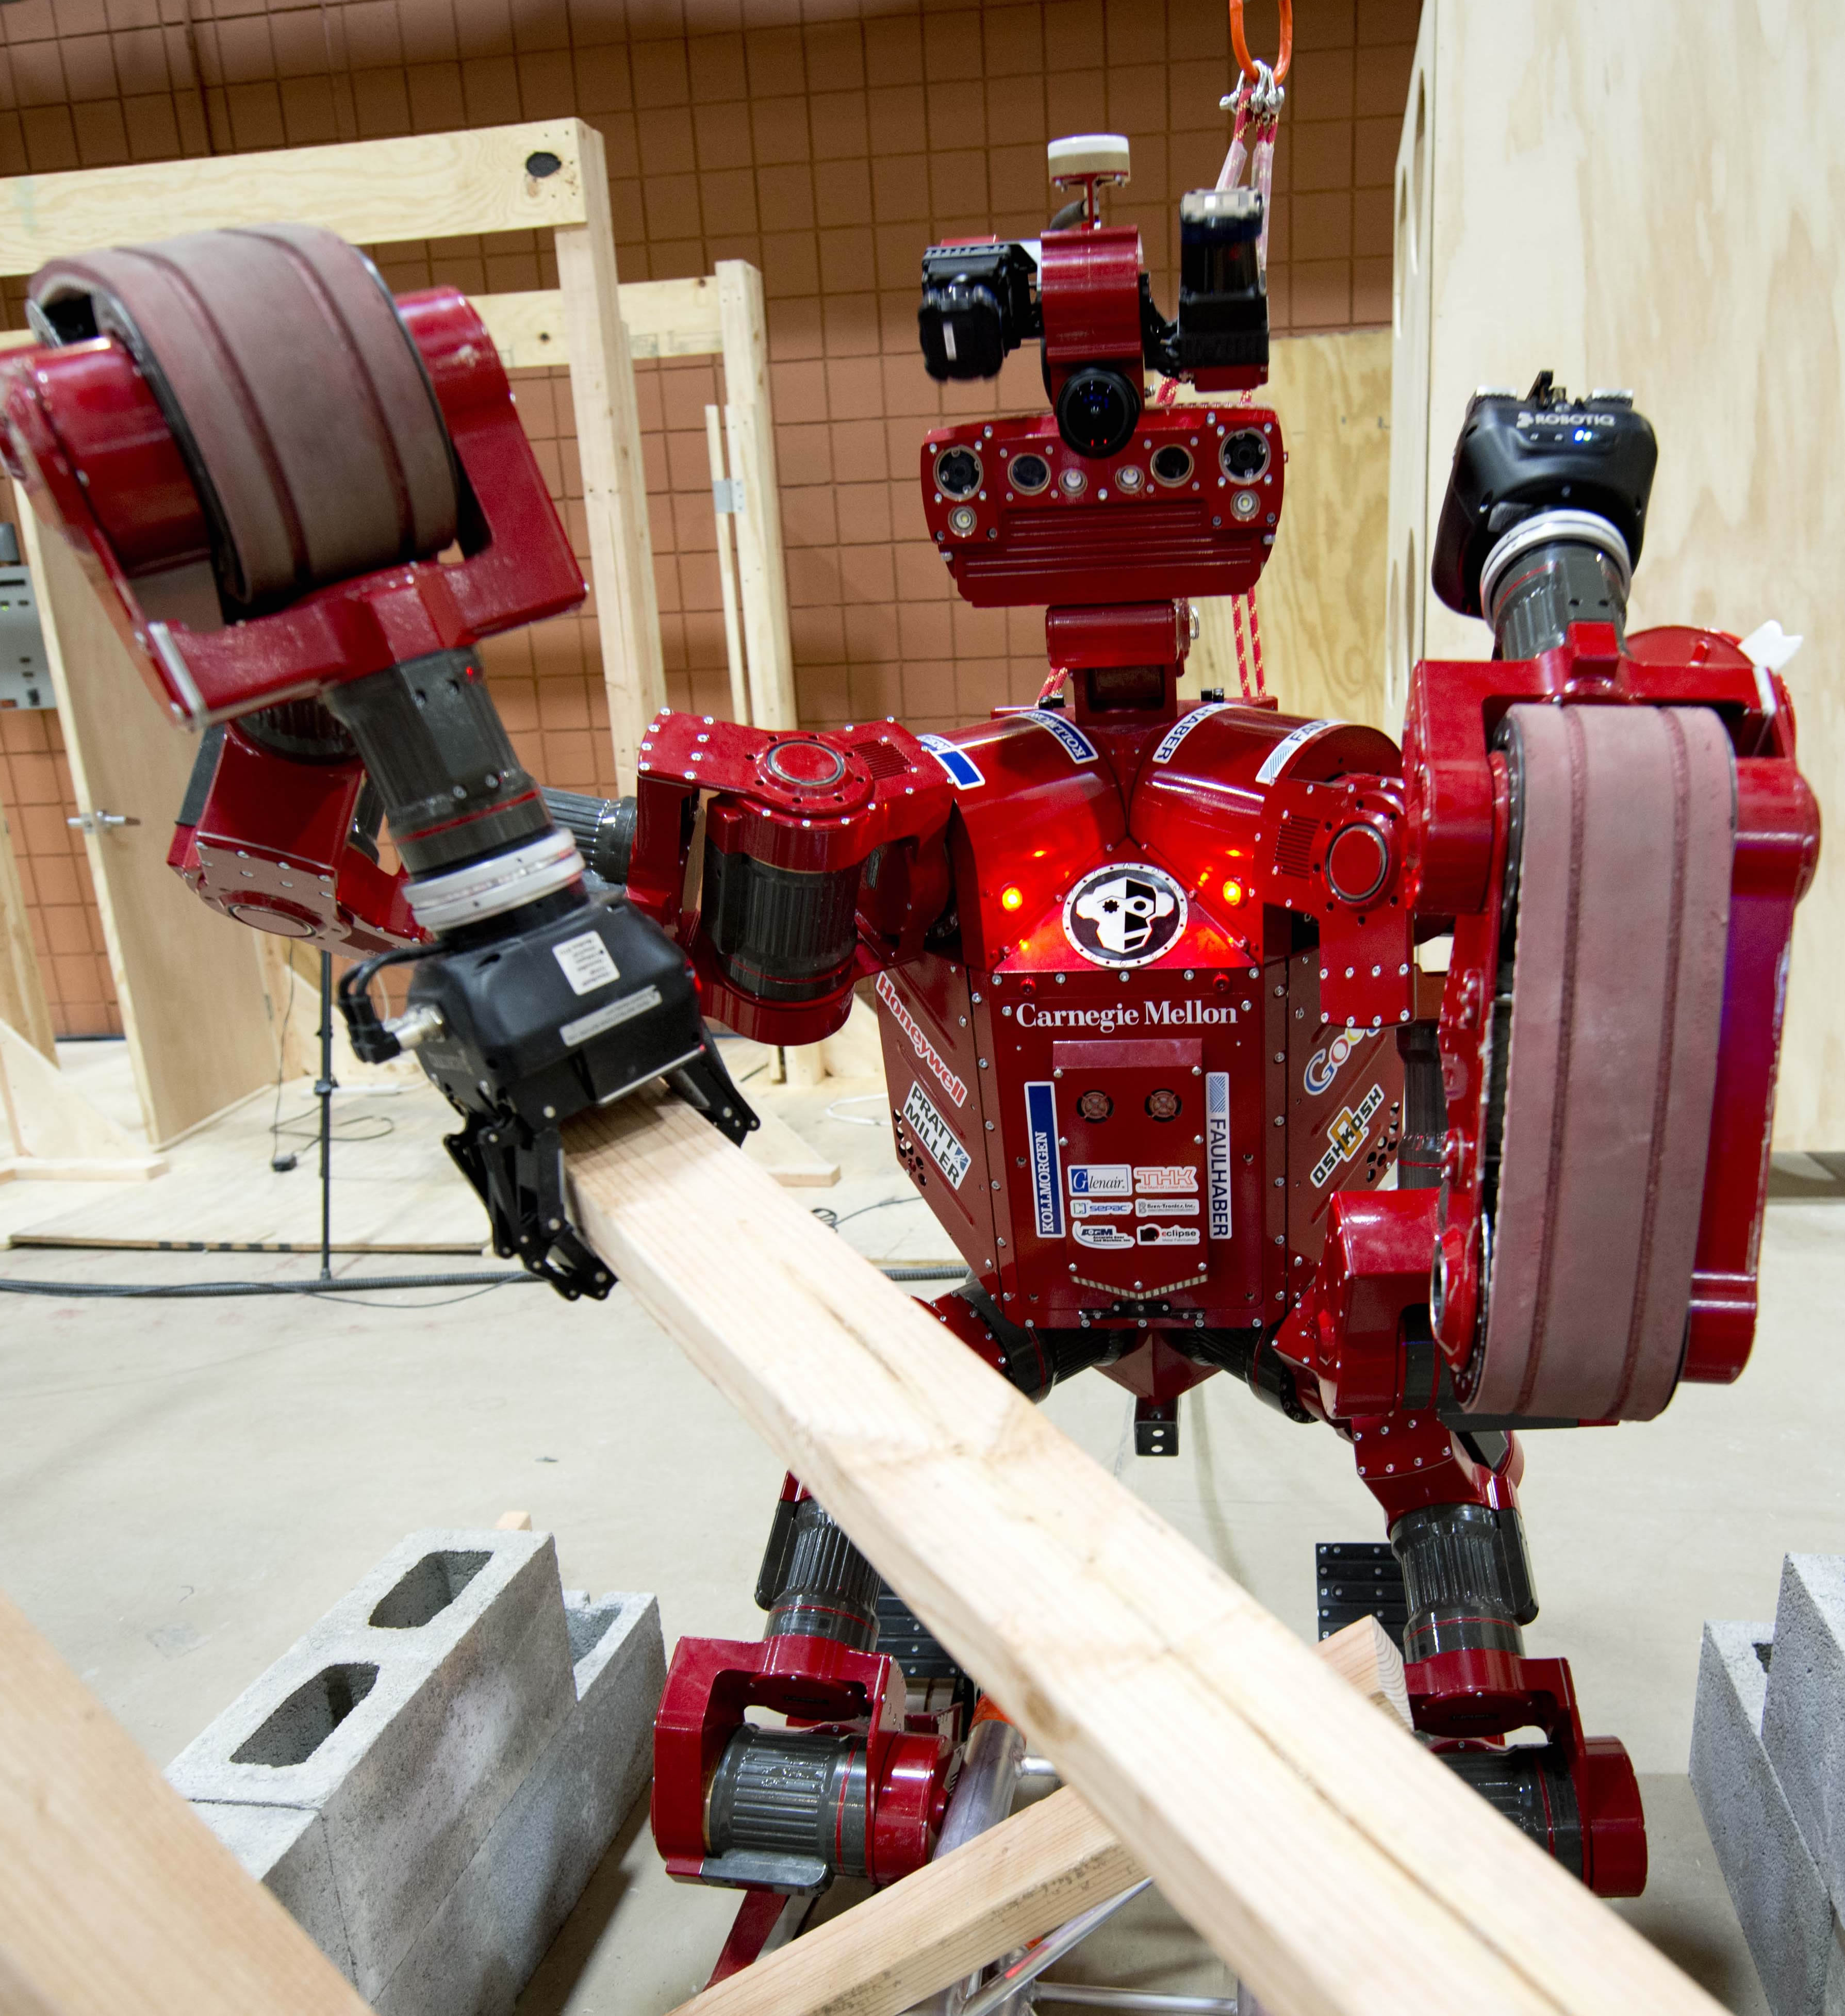
\includegraphics[height=2in]{figs/chimp-debris.jpg}
%      \end{center}
%      \caption{CHIMP Robot}
%   \end{subfigure}
%   \caption{Manipulation problems.}
%\end{widepage}
%\end{figure}


\newpage
\chapter{Introduction}

The steady advancement of technology
has automated an increasing variety of menial or dangerous tasks
previously performed by humans.
Computer algorithms now trade our stocks,
route our telephone calls and packages,
and fly our planes,
and simple machines clean our clothes and wash our dishes.

More complex tasks require complex robots with many
degrees of freedom.
Manipulation tasks, in particular,
present challenges in many areas including
perception, symbolic reasoning, and motion planning.
Successful applications have so far been largely
confined to large-scale manufacturing domains,
whose prescribed and structured environments
allow these challenges to be overcome.

However,
manipulation tasks such as clearing a kitchen table
or moving debris in a dangerous disaster scenario
can not yet be planned for quickly and reliably.
\begin{quote}
\emph{%
This thesis proposes an
efficient and robust motion planning approach
well-suited
to articulated robots
performing recurring manipulation tasks
in dynamic, unstructured environments.
}
\end{quote}

We outline the general structure of multi-step manipulation planning
in Chapter~\ref{chap:formulation}.
There are two principal challenges inherent in
human-scale manipulation tasks
that must be addressed by such approaches,
which we review here.

\textbf{Challenge 1: Task Efficiency.}

Autonomous systems performing manipulation tasks are
resource-constrained.
If a home robot takes thirty minutes to clear a table,
or a disaster response robot exhausts its battery ten minutes
into its mission,
these robots will not see widespread use.
These metrics are only meaningful
when applied across the entire task,
from the point it is assigned to the robot
to the point it is complete.

In order to accomplish such a manipulation task,
an autonomous robot must expend two types of effort.
First, it must allocate computation to \emph{plan}
a sequence of motions that will acheive the task.
Second, it must \emph{execute} these plans using its actuators.
Generally, there is a tradeoff between these two;
spending more effort during planning produces paths that are
cheaper to execute.
Planning costs are dominated by \emph{validity checking} --
e.g. checking whether configurations are free from collision.

Robots performing real-world human-scale manipulation tasks
tend to expend comparable effort in these two areas
(see Figure~\ref{fig:plan-exec-cost}).
While some approaches (e.g. anytime planning) attempt to capture
this tradeoff,
our approach,
the Greedy PRM (Chapter~\ref{chap:inflate}),
instead explicitly optimizes for both planning
and execution effort
given a planning effort model.
This allows the planner to determine the proper allocation of effort
between planning and execution in order to minimize total task cost.

Next, Chapter~\ref{chap:graphs-in-continuous}
discusses how to embed these roadmaps efficiently
into continuous configuration spaces,
touching on completeness,
efficiency, etc.

{
\setlength{\offsetpage}{0.5in}
\begin{figure}
\begin{widepage}
\begin{center}
   \begin{subfigure}[b]{1.4in}
      \begin{center}
\begin{tikzpicture}
\node at (0,0) {
   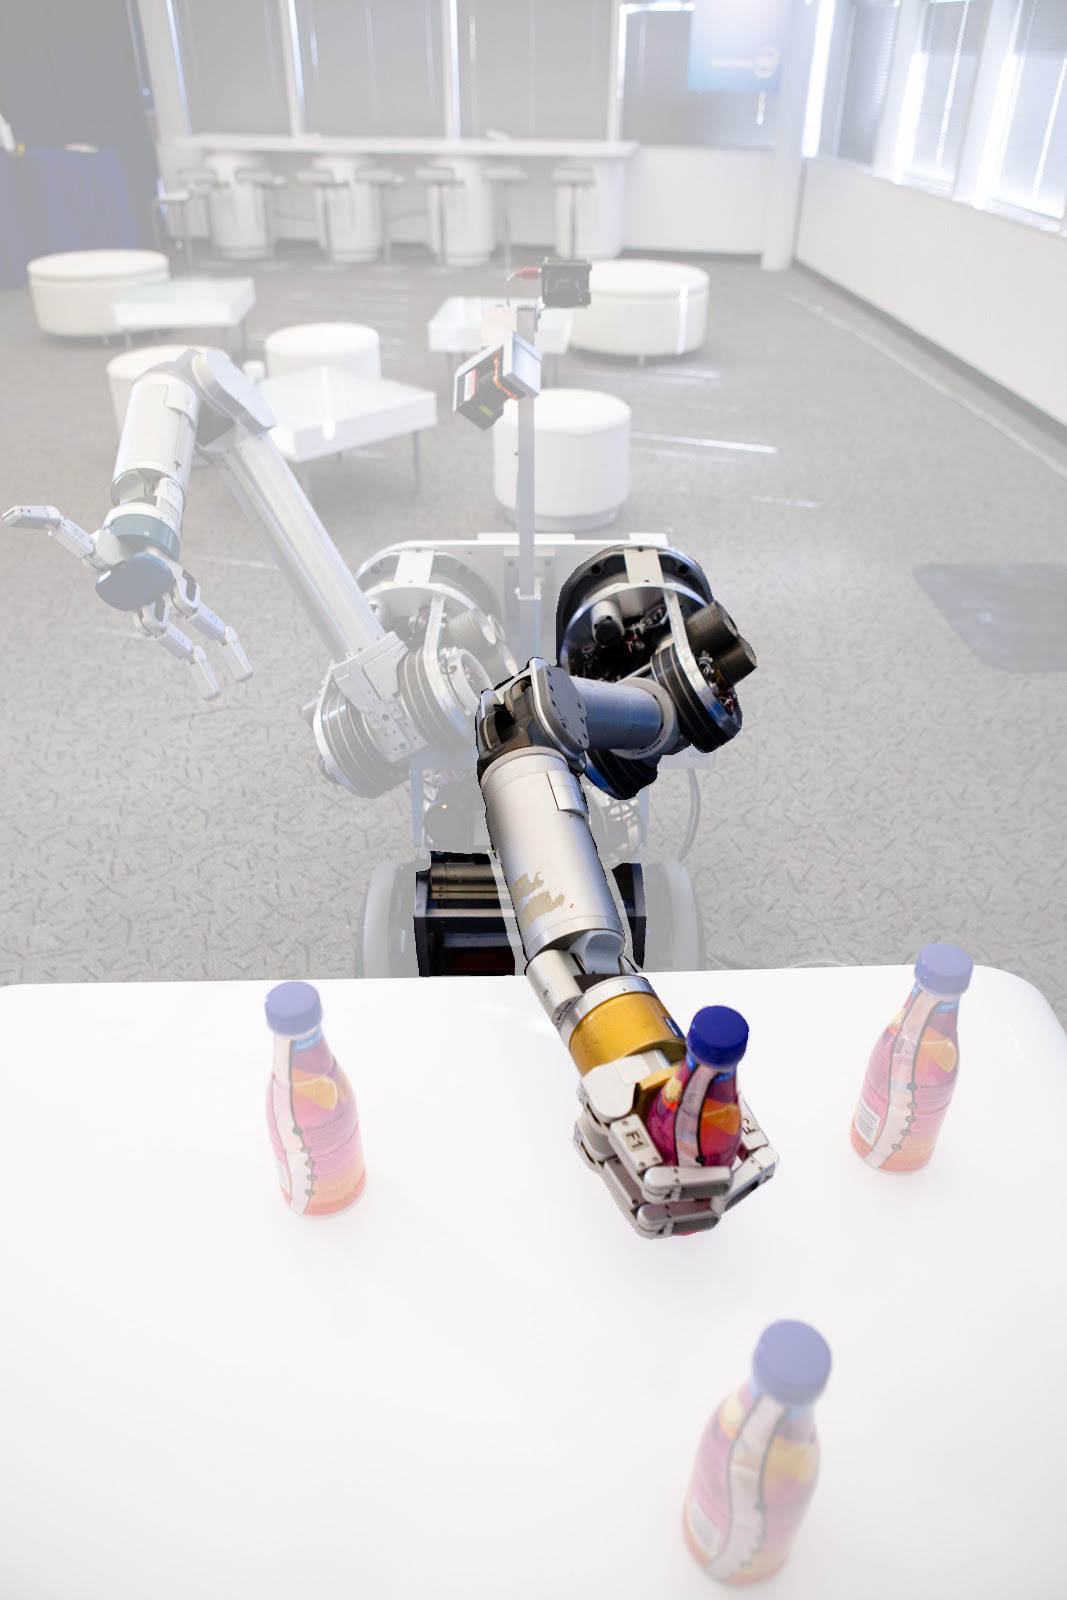
\includegraphics[height=2in]{figs/herb-fuze-cost.jpg}
};
\node[black,fill=white,fill opacity=0.5,text opacity=1]
   (planlab) at (-0.5,2.15) {Planning Cost};
\draw[->,thick] (planlab.south) -- (-0.3,-0.1);
\node[black,fill=white,fill opacity=0.5,text opacity=1]
   (execlab) at (0.5,-2.2) {Execution Cost};
\draw[->,thick] (execlab.north) -- (0.6,-1.4);
\end{tikzpicture}
      \end{center}
      \caption{\textsc{Herb} Home Robot}
   \end{subfigure}%
   \quad%
   \begin{subfigure}[b]{2.0in}
      \begin{center}
\begin{tikzpicture}
\node at (0,0) {
   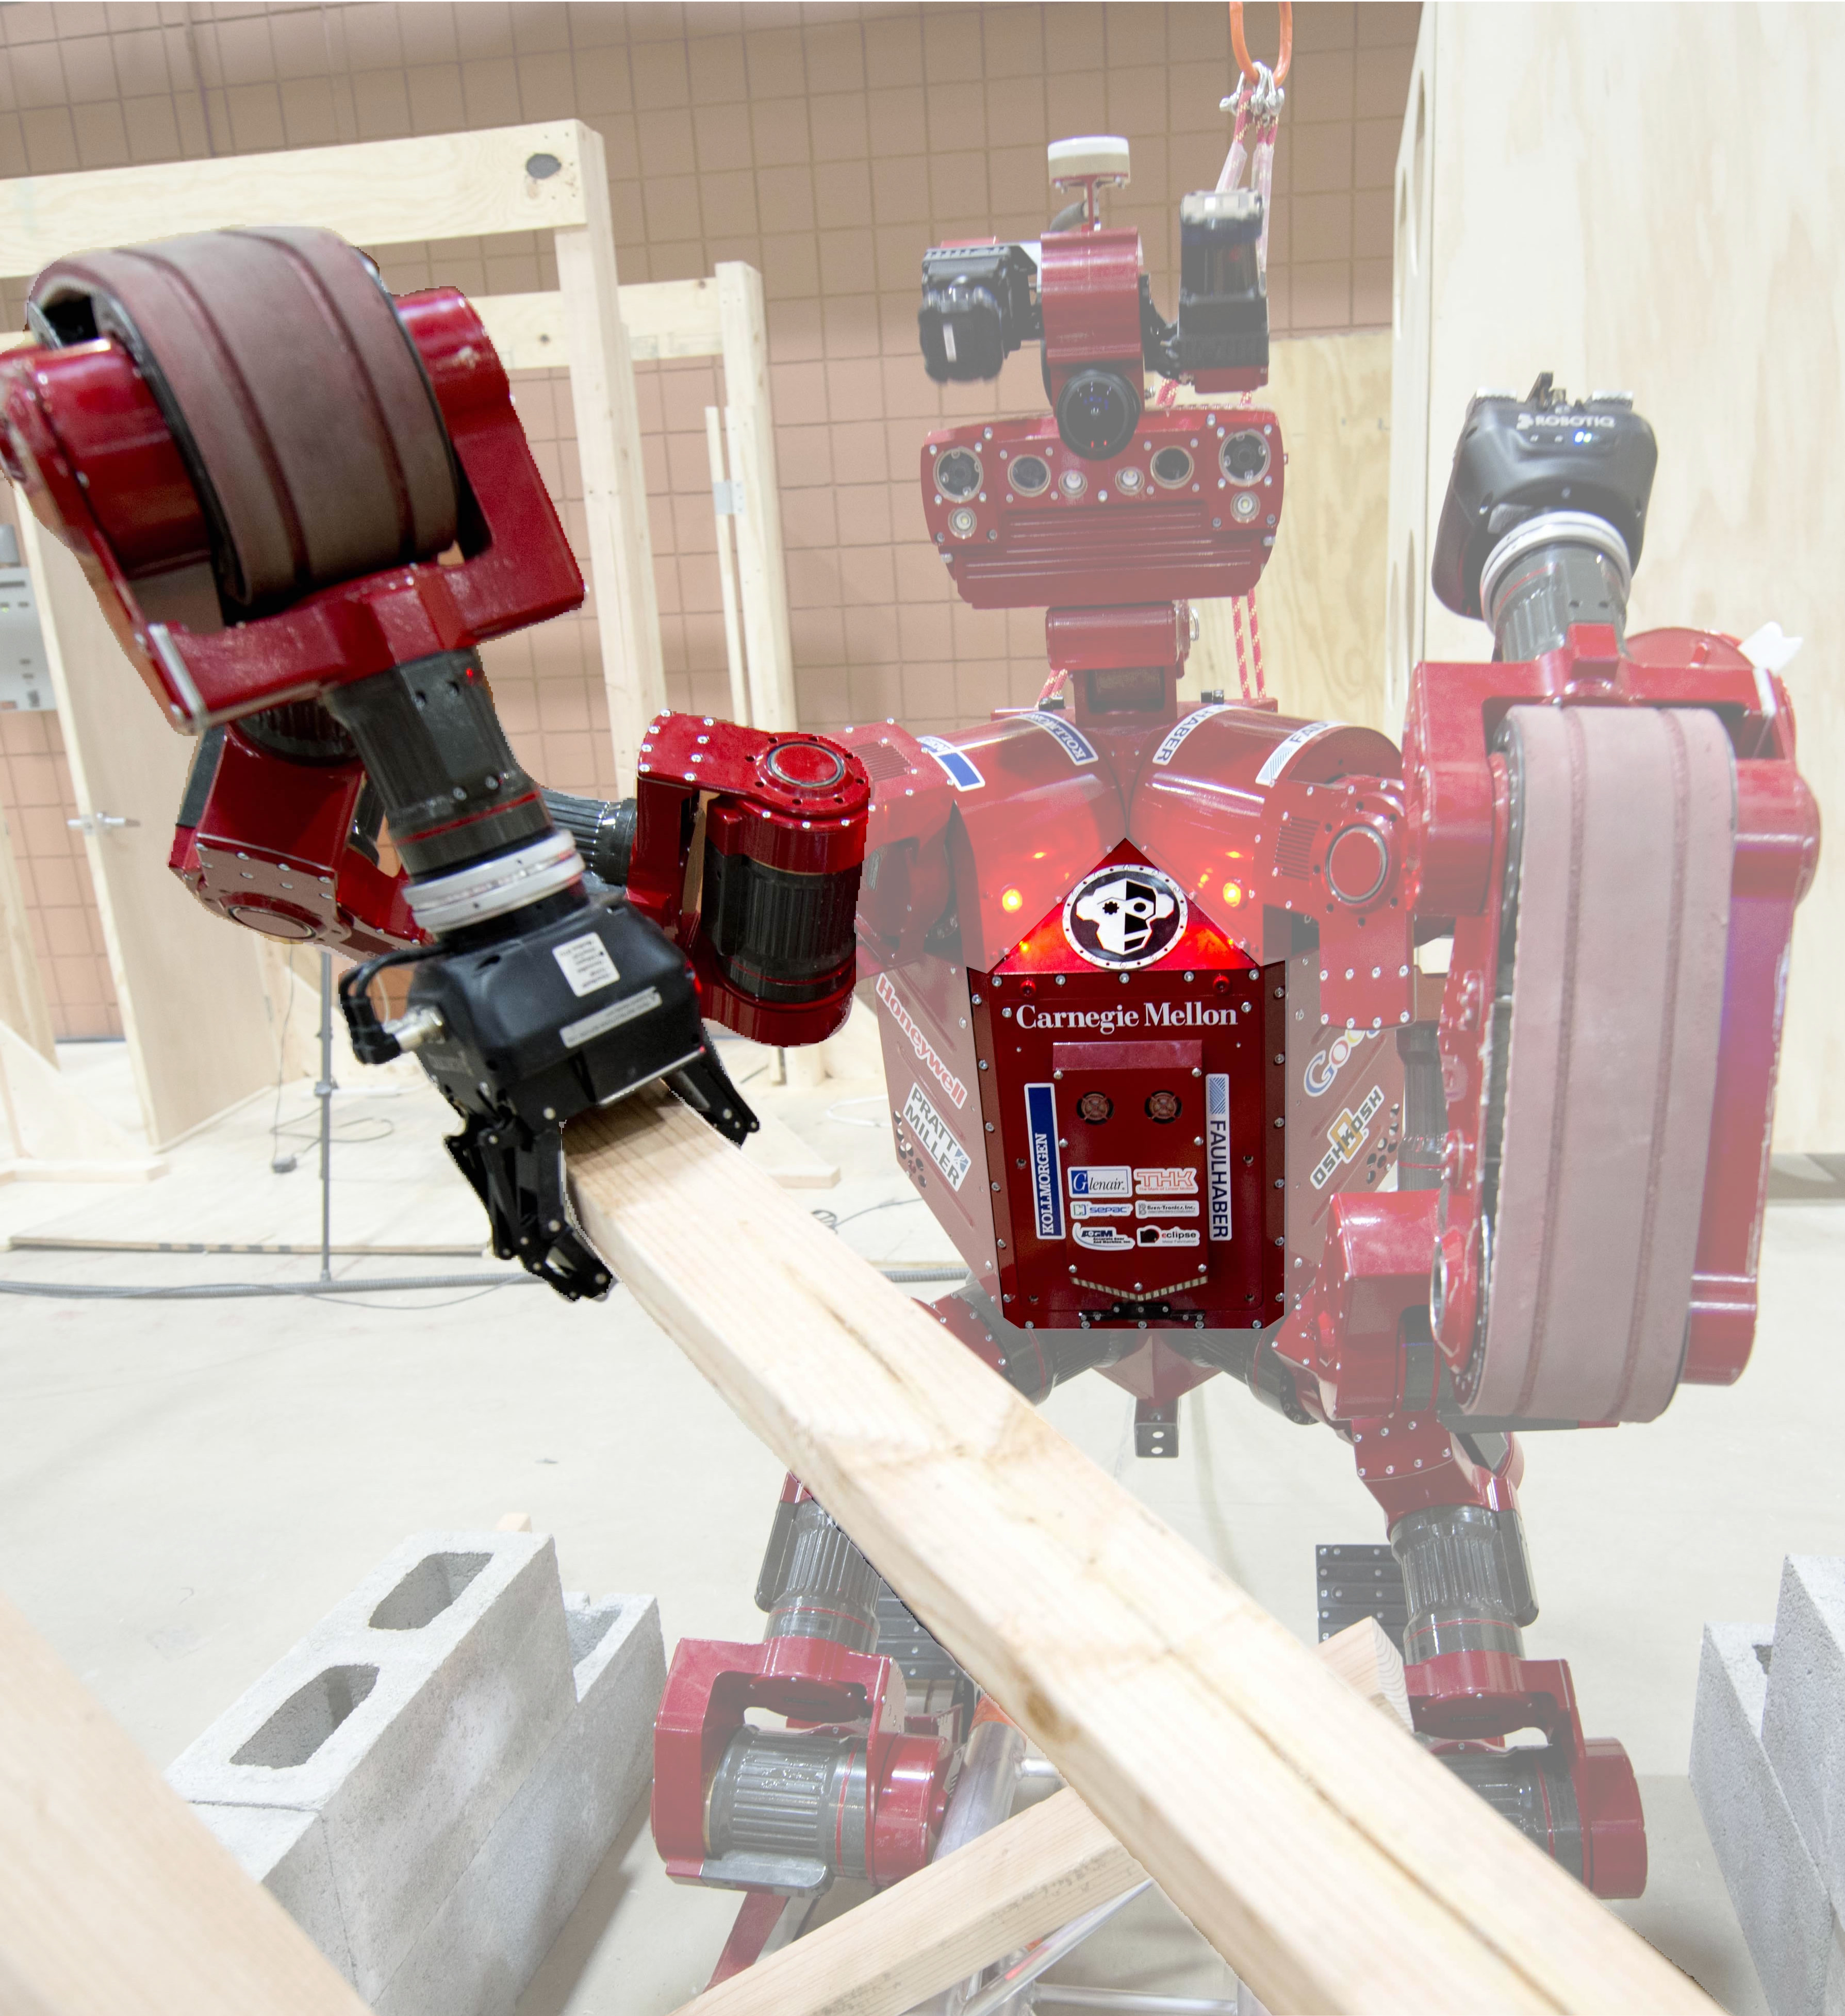
\includegraphics[height=2in]{figs/chimp-debris-cost.jpg}
};
\node[black,fill=white,fill opacity=0.5,text opacity=1]
   (planlab) at (1.0,2.15) {Planning Cost};
\draw[->,thick] (planlab.south) -- (0.6,0.6);
\node[black,fill=white,fill opacity=0.5,text opacity=1]
   (execlab) at (-0.9,-2.2) {Execution Cost};
\draw[->,thick] (execlab.north) -- (-1.1,-0.8);
\end{tikzpicture}
      \end{center}
      \caption{\textsc{Chimp} Disaster Response Robot}
   \end{subfigure}%
   \quad%
   \begin{subfigure}[b]{2.0in}
      \begin{center}
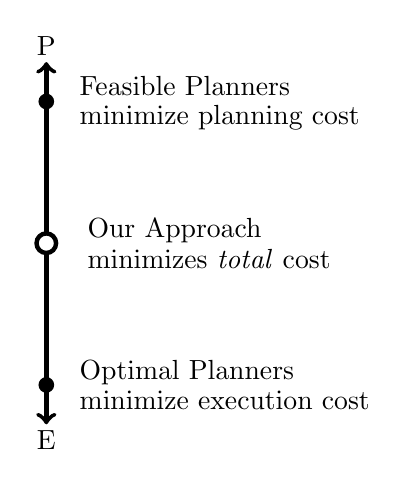
\begin{tikzpicture}
\draw[<->,ultra thick] (0,-2.3) -- (0,2.3);
\node at (0,2.5) {P};
\node at (0,-2.5) {E};
\node[circle,fill=black,inner sep=2] at (0,1.8) {};
\node[circle,fill=black,inner sep=2] at (0,-1.8) {};
\node[circle,draw,ultra thick,fill=white,inner sep=2.5] at (0,0) {};
\node[anchor=west] at (0.3,2.0) {Feasible Planners};
\node[anchor=west] at (0.3,1.6) {minimize planning cost};
\node[anchor=west] at (0.4, 0.16) {Our Approach};
\node[anchor=west] at (0.4,-0.2) {minimizes \emph{total} cost};
\node[anchor=west] at (0.3,-1.64) {Optimal Planners};
\node[anchor=west] at (0.3,-2.0) {minimize execution cost};
\end{tikzpicture}
      \end{center}
      \caption{Planning vs. Execution Cost}
   \end{subfigure}
   \caption{For manipulation tasks,
      both the \textsc{Herb} \cite{srinivasa2012herb20}
      and \textsc{Chimp} \cite{stentz2014chimp} robots
      incur comparable cost (e.g. time or energy)
      during planning and execution.
      Our approach considers both explicitly.}
   \label{fig:plan-exec-cost}
\end{center}
\end{widepage}
\end{figure}
}

\textbf{Challenge 2: Sub-Problem Structure.}

While planning cost is a significant component
in resource-constrained human-scale problems,
manipulation tasks exhibit a structure
which makes it difficult to apply fast planning approaches.
In particular,
they are inherently composed of multiple distinct sub-problems,
each of which 
must be validated a different subset of configuration space.
For example, see the manipulation task in
Figure~\ref{fig:intro-multi-step}.

We could do na\"{\i}ve planning, like in the
DRC Trials \cite{dellin2014drc},
with no reuse.
We call a single-query planner for each step.
Either we generate roots at the start,
or we let each sub-planner pick a root it can get to, and commit.
First, we can get stuck,
comitting to something that either is infeasible, or takes too long.
Second, this is too slow --
each sub-plan simply takes too long.

We could try multi-query planning,
but as mentioned,
the valid subset changes for each step.

We solve this in two ways.
First, in Chapter~\ref{chap:multi-set},
we introduce the multi-set planning problem.
We show that while the valid subsets are different for each step,
they are related in a structured way.
In fact, we show how lots of different prior ideas for planner
efficiency are unified by this formalism.

Second, Chapter~\ref{chap:multi-set-prm}
uses the multi-set formalism as a planning cost model
for use by the Greedy PRM.
The resulting algorithm,
the Multi-Set PRM,
uses propositional logic to represent multi-set stuff
algorithmically.
We show how we can incremental graph search approaches
to make it super fast.

{
\setlength{\offsetpage}{0.75in}
\begin{figure}
\begin{widepage}
\begin{center}

\begin{subfigure}[t]{0.19\linewidth}
\centering
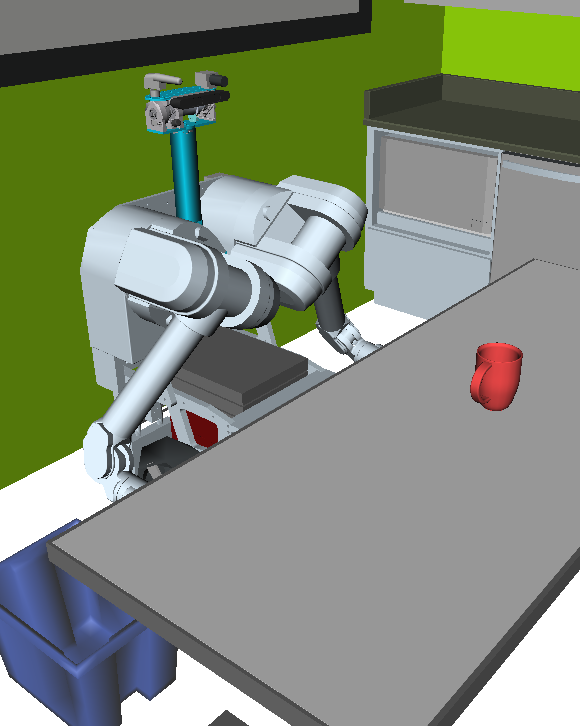
\includegraphics[width=\columnwidth]{figs/testherb-a.png}
\caption{Start config}
\end{subfigure}
\begin{subfigure}[t]{0.19\linewidth}
\centering
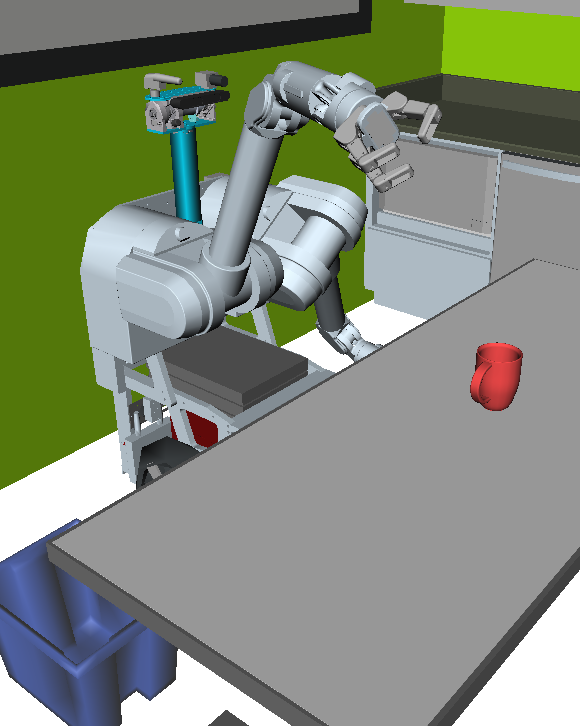
\includegraphics[width=\columnwidth]{figs/testherb-b.png}
\caption{Step 1 in $X_1$}
\end{subfigure}
\begin{subfigure}[t]{0.19\linewidth}
\centering
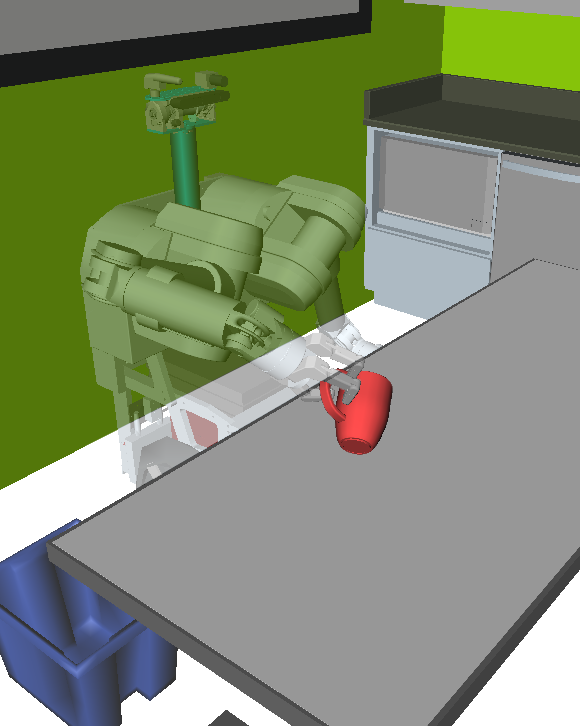
\includegraphics[width=\columnwidth]{figs/testherb-c.png}
\caption{Step 2 in $X_2$}
\end{subfigure}
\begin{subfigure}[t]{0.19\linewidth}
\centering
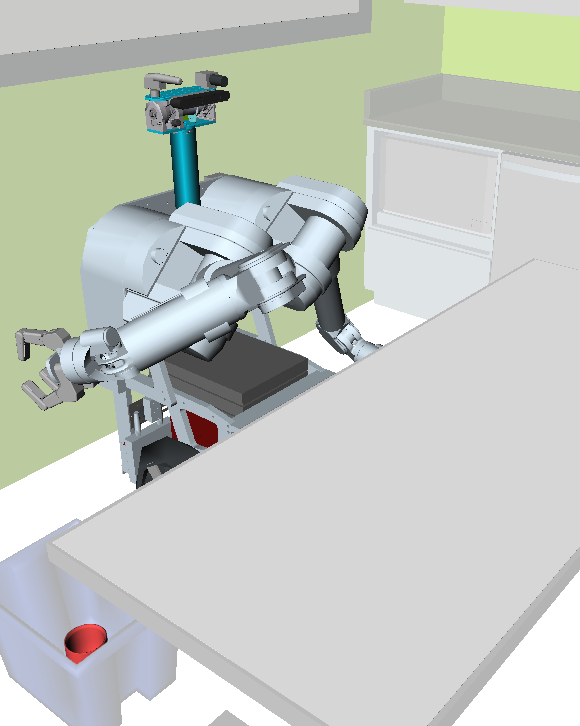
\includegraphics[width=\columnwidth]{figs/testherb-d.png}
\caption{Step 3 in $X_3$}
\end{subfigure}
\begin{subfigure}[t]{0.19\linewidth}
\centering
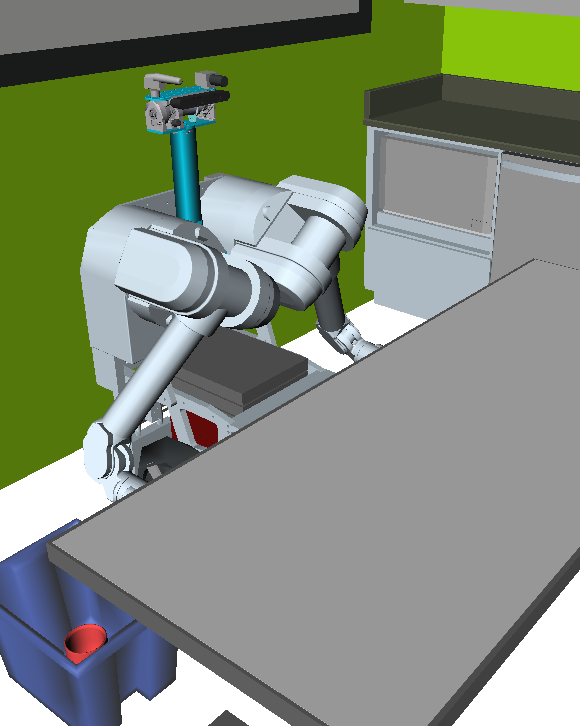
\includegraphics[width=\columnwidth]{figs/testherb-e.png}
\caption{End config}
\end{subfigure}

\vspace{0.1in}

   \begin{subfigure}[b]{4.0in}
      \begin{center}
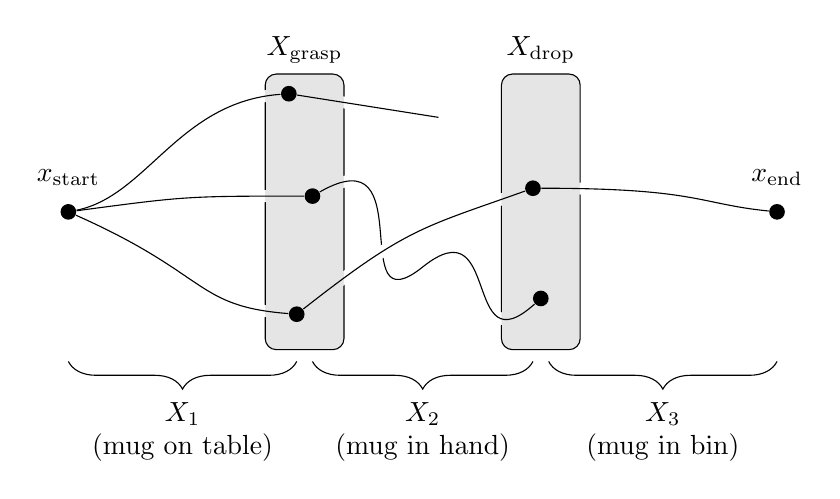
\begin{tikzpicture}
\node[draw,black,rounded corners,minimum height=3.5cm,minimum width=1cm]
   (Xgrasp) at (3,0) {};
\node[draw,black,rounded corners,minimum height=3.5cm,minimum width=1cm]
   (Xdrop) at (6,0) {};
\node[circle,fill=black,inner sep=2] (xstart) at (0,0) {};
\node[circle,fill=black,inner sep=2] (xg1) at (2.8,1.5) {};
\node[circle,fill=black,inner sep=2] (xg2) at (3.1,0.2) {};
\node[circle,fill=black,inner sep=2] (xg3) at (2.9,-1.3) {};
\node[circle,fill=black,inner sep=2] (xd1) at (5.9,0.3) {};
\node[circle,fill=black,inner sep=2] (xd2) at (6.0,-1.1) {};
\node[circle,fill=black,inner sep=2] (xend) at (9,0) {};
\node[above=0.1cm of xstart] {$x_{\mbox{\scriptsize start}}$};
\node[above=0cm of Xgrasp] {$X_{\mbox{\scriptsize grasp}}$};
\node[above=0cm of Xdrop] {$X_{\mbox{\scriptsize drop}}$};
\node[above=0.1cm of xend] {$x_{\mbox{\scriptsize end}}$};

\draw[line width=1.5mm,white]
   (xstart)
   .. controls (1,0.2) and (1.4,1.4) .. (xg1)
   -- (4.7,1.2);
\draw[line width=1.5mm,white]
   (xstart)
   .. controls (1.5,0.2) .. (xg2)
   .. controls (4.5,1) and (3.5,-1.5) .. (4.5,-0.7)
   .. controls (5.5,0.1) and (5.0,-2) .. (xd2);
\draw[line width=1.5mm,white]
   (xstart)
   .. controls (1.8,-0.8) and (1.6,-1.2) .. (xg3);

\draw
   (xstart)
   .. controls (1,0.2) and (1.4,1.4) .. (xg1)
   -- (4.7,1.2);
\draw
   (xstart)
   .. controls (1.5,0.2) .. (xg2)
   .. controls (4.5,1) and (3.5,-1.5) .. (4.5,-0.7)
   .. controls (5.5,0.1) and (5.0,-2) .. (xd2);
\draw[line width=1.5mm,white]
   (xg3)
   .. controls (4.3,-0.2) and (4.5,-0.2) .. (xd1)
   .. controls (8,0.3) and (8,0.1) .. (xend);
\draw
   (xstart)
   .. controls (1.8,-0.8) and (1.6,-1.2) .. (xg3)
   .. controls (4.3,-0.2) and (4.5,-0.2) .. (xd1)
   .. controls (8,0.3) and (8,0.1) .. (xend);

\node[fill,black,rounded corners,minimum height=3.5cm,minimum width=1cm,
   opacity=0.1] at (3,0) {};
\node[fill,black,rounded corners,minimum height=3.5cm,minimum width=1cm,
   opacity=0.1] at (6,0) {};

\draw [decorate,decoration={brace,mirror,amplitude=10pt}]
(0.0,-1.9) -- (2.9,-1.9) node [black,midway,yshift=-0.9cm,align=center]
   {$X_1$\\(mug on table)};

\draw [decorate,decoration={brace,mirror,amplitude=10pt}]
(3.1,-1.9) -- (5.9,-1.9) node [black,midway,yshift=-0.9cm,align=center]
   {$X_2$\\(mug in hand)};

\draw [decorate,decoration={brace,mirror,amplitude=10pt}]
(6.1,-1.9) -- (9.0,-1.9) node [black,midway,yshift=-0.9cm,align=center]
   {$X_3$\\(mug in bin)};

\end{tikzpicture}
      \end{center}
      \caption{Plan sequences
         within distinct free $\mathcal{C}$-subsets
         from the problem above.}
   \end{subfigure}%
   \quad%
   \begin{subfigure}[b]{2.0in}
      \begin{center}
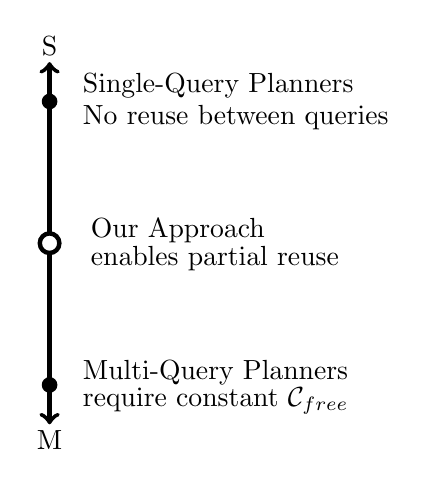
\begin{tikzpicture}
\draw[<->,ultra thick] (0,-2.3) -- (0,2.3);
\node at (0,2.5) {S};
\node at (0,-2.5) {M};
\node[circle,fill=black,inner sep=2] at (0,1.8) {};
\node[circle,fill=black,inner sep=2] at (0,-1.8) {};
\node[circle,draw,ultra thick,fill=white,inner sep=2.5] at (0,0) {};
\node[anchor=west] at (0.3,2.0) {Single-Query Planners};
\node[anchor=west] at (0.3,1.6) {No reuse between queries};
\node[anchor=west] at (0.4, 0.16) {Our Approach};
\node[anchor=west] at (0.4,-0.2) {enables partial reuse};
\node[anchor=west] at (0.3,-1.64) {Multi-Query Planners};
\node[anchor=west] at (0.3,-2.0) {require constant $\mathcal{C}_{free}$};
\end{tikzpicture}
      \end{center}
      \caption{Single vs. Multi Query Planners}
   \end{subfigure}
   \caption{\textsc{Herb} plans for a simple manipulation task
      to grasp, transfer, and drop a mug from a table into a bin
      before returning to an end configuration.
      Each sub-problem requires a path in a distinct free subset of
      configuration space;
      our approach enables partial reuse between these steps.}
   \label{fig:intro-multi-step}
\end{center}
\end{widepage}
\end{figure}
}

\textbf{Applications and Experiments}

We give a bunch of examples of this framework
for different robots.
For example, I really want to talk about robots idly
hypothesizing worlds.

{
\setlength{\offsetpage}{0.75in}
\begin{figure}
\begin{widepage}
\begin{center}
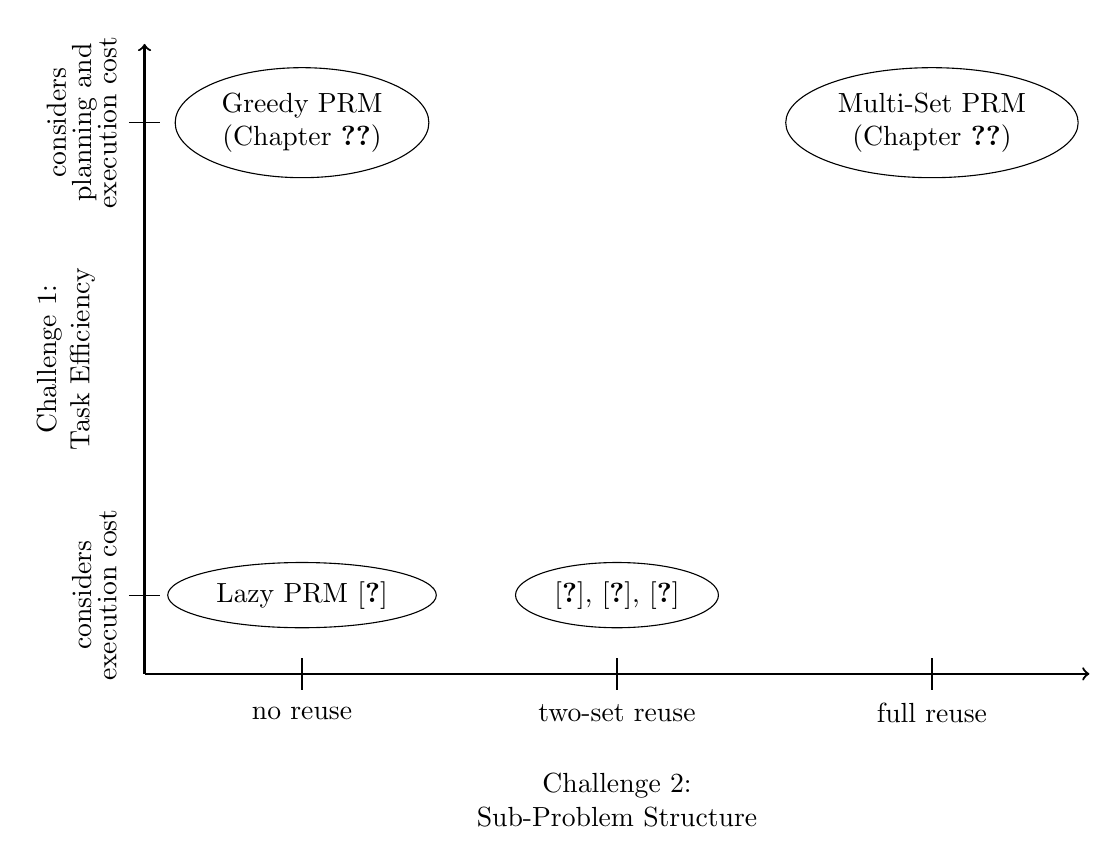
\begin{tikzpicture}

% axes
\draw[->,thick] (0,0) -- (0,8); 
\draw[->,thick] (0,0) -- (12,0);
\node[rotate=90,align=center] at (-1.0,4)
   {Challenge 1:\\Task Efficiency};
\node[align=center] at (6,-1.6)
   {Challenge 2:\\Sub-Problem Structure};

% y tics
\draw (-0.2,1) -- (0.2,1);
\node[rotate=90,align=center] at (-0.64,1)
   {considers\\[-0.04in]execution cost};
\draw (-0.2,7) -- (0.2,7);
\node[rotate=90,align=center] at (-0.8,7)
   {considers\\[-0.04in]planning and\\[-0.04in]execution cost};

% x tics
\draw (2,-0.2) -- (2,0.2);
\node[align=center] at (2,-0.5) {no reuse};
\draw (6,-0.2) -- (6,0.2);
\node[align=center] at (6,-0.5) {two-set reuse};
\draw (10,-0.2) -- (10,0.2);
\node[align=center] at (10,-0.5) {full reuse};

% algorithms
\node[draw,ellipse,align=center] at (2,1)
   {Lazy PRM \cite{bohlin2000lazyprm}};

\node[draw,ellipse,align=center] at (6,1)
   {\cite{leven2000changing}, \cite{kallman2004dynamicroadmaps},
   \cite{jaillet2004dynamicprm}};

\node[draw,ellipse,align=center] at (2,7)
   {Greedy PRM\\(Chapter~\ref{chap:inflate})};

\node[draw,ellipse,align=center] at (10,7)
   {Multi-Set PRM\\(Chapter~\ref{chap:multi-set-prm})};

\end{tikzpicture}
\caption{Graphical outline of $\mathcal{C}$-space planners.
   Work in progress.}
\label{fig:graphical-outline}
\end{center}
\end{widepage}
\end{figure}
}



\newpage
\chapter{Sub-Problems in Manipulation Planning}
\label{chap:formulation}

In this chapter,
we lay out the structure of the manipulation planning problem.

\section{Sub-Problem Structure}

\begin{figure}
\begin{widepage}
\begin{center}
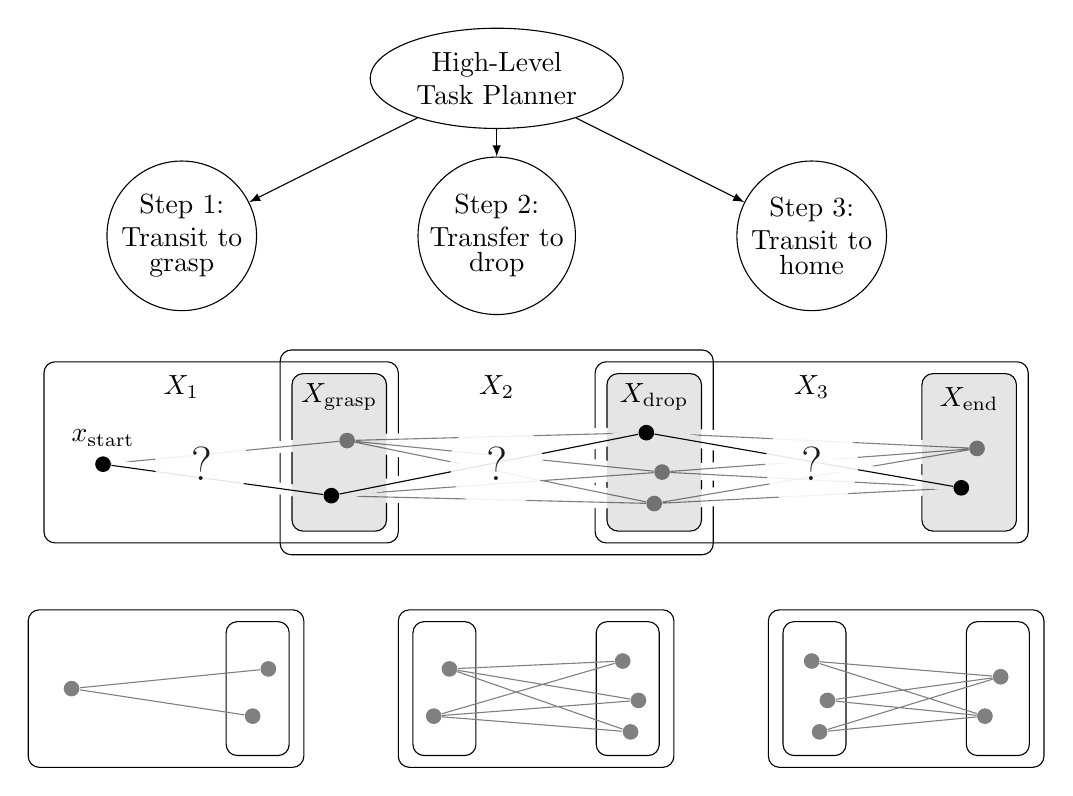
\begin{tikzpicture}
\tikzset{>=latex} % arrow heads

% top: symbolic planner
\node[draw,ellipse,align=center] (high) at (0,0)
   {High-Level\\Task Planner};
\node[draw,circle,align=center,inner sep=0,minimum size=1.9cm] (step1) at (-4,-2)
   {Step 1:\\Transit to\\[-0.04in]grasp};
\node[draw,circle,align=center,inner sep=0,minimum size=1.9cm] (step2) at (0,-2)
   {Step 2:\\Transfer to\\[-0.04in]drop};
\node[draw,circle,align=center,inner sep=0,minimum size=1.9cm] (step3) at (4,-2)
   {Step 3:\\Transit to\\[-0.04in]home};
\draw[->] (high) -> (step1);
\draw[->] (high) -> (step2);
\draw[->] (high) -> (step3);

% middle: c-space sequence
% valid subsets
\node[draw,black,rounded corners,
   minimum height=2.3cm,minimum width=4.5cm]
   (X1) at (-3.5,-4.75) {};
\node[draw,black,rounded corners,
   minimum height=2.6cm,minimum width=5.5cm]
   (X2) at (0,-4.75) {};
\node[draw,black,rounded corners,
   minimum height=2.3cm,minimum width=5.5cm]
   (X3) at ( 4,-4.75) {};
% root sets
\node[draw,black,rounded corners,
   minimum height=2cm,minimum width=1.2cm]
   (Xgrasp) at (-2,-4.75) {};
\node[draw,black,rounded corners,
   minimum height=2cm,minimum width=1.2cm]
   (Xdrop) at (2,-4.75) {};
\node[draw,black,rounded corners,
   minimum height=2cm,minimum width=1.2cm]
   (Xend) at (6,-4.75) {};
% set labels
\node[above=-0.6cm of Xgrasp] {$X_{\mbox{\scriptsize grasp}}$};
\node[above=-0.6cm of Xdrop] {$X_{\mbox{\scriptsize drop}}$};
\node[above=-0.6cm of Xend] {$X_{\mbox{\scriptsize end}}$};
\node[above left=-0.6cm and -2.1cm of X1] {$X_1$};
\node[above=-0.75cm of X2] {$X_2$};
\node[above=-0.6cm of X3] {$X_3$};
% nodes and paths
\node[circle,fill=black,inner sep=2] (xstart) at (-5,-4.9) {};
\node[circle,fill=black!50,inner sep=2] (xg1) at (-1.9,-4.6) {};
\node[circle,fill=black,inner sep=2] (xg2) at (-2.1,-5.3) {};
\node[circle,fill=black,inner sep=2] (xd1) at ( 1.9,-4.5) {};
\node[circle,fill=black!50,inner sep=2] (xd2) at ( 2.1,-5.0) {};
\node[circle,fill=black!50,inner sep=2] (xd3) at ( 2.0,-5.4) {};
\node[circle,fill=black!50,inner sep=2] (xe1) at ( 6.1,-4.7) {};
\node[circle,fill=black,inner sep=2] (xe2) at ( 5.9,-5.2) {};
\node[above=0cm of xstart] {$x_{\mbox{\scriptsize start}}$};
% lines
\draw[line width=1.5mm,white]
   (xstart) -- (xg1) (xg1) -- (xd1) (xg1) -- (xd2) (xg1) -- (xd3)
   (xg2) -- (xd2) (xg2) -- (xd3) (xd1) -- (xe1) (xd2) -- (xe1)
   (xd2) -- (xe2) (xd3) -- (xe1) (xd3) -- (xe2);
\draw[draw=black!50]
   (xstart) -- (xg1) (xg1) -- (xd1) (xg1) -- (xd2) (xg1) -- (xd3)
   (xg2) -- (xd2) (xg2) -- (xd3) (xd1) -- (xe1) (xd2) -- (xe1)
   (xd2) -- (xe2) (xd3) -- (xe1) (xd3) -- (xe2);
\draw[line width=1.5mm,white]
   (xstart) -- (xg2) (xg2) -- (xd1) (xd1) -- (xe2);
\draw
   (xstart) -- (xg2) (xg2) -- (xd1) (xd1) -- (xe2);
% grey sets (overlay)
\node[fill=black,opacity=0.1,rounded corners,
   minimum height=2cm,minimum width=1.2cm]
   at (-2,-4.75) {};
\node[fill=black,opacity=0.1,rounded corners,
   minimum height=2cm,minimum width=1.2cm]
   at (2,-4.75) {};
\node[fill=black,opacity=0.1,rounded corners,
   minimum height=2cm,minimum width=1.2cm]
   at (6,-4.75) {};
% question mark bubbles
\node[circle,fill=white,fill opacity=0.9,inner sep=7pt]
   at (-3.75,-4.9) {\LARGE ?};
\node[circle,fill=white,fill opacity=0.9,inner sep=7pt]
   at (0,-4.9) {\LARGE ?};
\node[circle,fill=white,fill opacity=0.9,inner sep=7pt]
   at (4.0,-4.9) {\LARGE ?};

% bottom: individual planner instances
\node[draw,black,rounded corners,
   minimum height=2cm,minimum width=3.5cm]
   (sm1) at (-4.2,-7.75) {};
\node[draw,black,rounded corners,
   minimum height=1.7cm,minimum width=0.8cm,
   right=-1cm of sm1] {};
\node[circle,fill=black!50,inner sep=2] (sm1xstart) at (-5.4,-7.75) {};
\node[circle,fill=black!50,inner sep=2] (sm1xg1) at (-2.9,-7.5) {};
\node[circle,fill=black!50,inner sep=2] (sm1xg2) at (-3.1,-8.1) {};
\draw[draw=black!50]
   (sm1xstart) -- (sm1xg1) (sm1xstart) -- (sm1xg2);

\node[draw,black,rounded corners,
   minimum height=2cm,minimum width=3.5cm]
   (sm2) at (0.5,-7.75) {};
\node[draw,black,rounded corners,
   minimum height=1.7cm,minimum width=0.8cm,
   left=-1cm of sm2] {};
\node[draw,black,rounded corners,
   minimum height=1.7cm,minimum width=0.8cm,
   right=-1cm of sm2] {};
\node[circle,fill=black!50,inner sep=2] (sm2xg1) at (-0.6,-7.5) {};
\node[circle,fill=black!50,inner sep=2] (sm2xg2) at (-0.8,-8.1) {};
\node[circle,fill=black!50,inner sep=2] (sm2xd1) at ( 1.6,-7.4) {};
\node[circle,fill=black!50,inner sep=2] (sm2xd2) at ( 1.8,-7.9) {};
\node[circle,fill=black!50,inner sep=2] (sm2xd3) at ( 1.7,-8.3) {};
\draw[draw=black!50]
   (sm2xg1) -- (sm2xd1) (sm2xg1) -- (sm2xd2) (sm2xg1) -- (sm2xd3)
   (sm2xg2) -- (sm2xd1) (sm2xg2) -- (sm2xd2) (sm2xg2) -- (sm2xd3);

\node[draw,black,rounded corners,
   minimum height=2cm,minimum width=3.5cm]
   (sm3) at ( 5.2,-7.75) {};
\node[draw,black,rounded corners,
   minimum height=1.7cm,minimum width=0.8cm,
   left=-1cm of sm3] {};
\node[draw,black,rounded corners,
   minimum height=1.7cm,minimum width=0.8cm,
   right=-1cm of sm3] {};
\node[circle,fill=black!50,inner sep=2] (sm3xd1) at ( 4.0,-7.4) {};
\node[circle,fill=black!50,inner sep=2] (sm3xd2) at ( 4.2,-7.9) {};
\node[circle,fill=black!50,inner sep=2] (sm3xd3) at ( 4.1,-8.3) {};
\node[circle,fill=black!50,inner sep=2] (sm3xe1) at ( 6.4,-7.6) {};
\node[circle,fill=black!50,inner sep=2] (sm3xe2) at ( 6.2,-8.1) {};
\draw[draw=black!50]
   (sm3xd1) -- (sm3xe1) (sm3xd1) -- (sm3xe2) (sm3xd2) -- (sm3xe1)
   (sm3xd2) -- (sm3xe2) (sm3xd3) -- (sm3xe1) (sm3xd3) -- (sm3xe2);

\end{tikzpicture}
\end{center}
\caption{This is a caption.}
\end{widepage}
\end{figure}

Show that figure again.

Briefly discuss the higher-level planner.
Not doing research here -- just need something that specifies
geometric goals.
Complementary to symbolic planners
or from humans (e.g. the DRC -- need cite).
For this proposal,
will only discuss seqential sub-plans,
but an intelligent meta-planner
can do non-sequential stuff too.

Multi-step problem structure (lots of options at each step);
decomposition into a bunch of "local planner" like things.
We're essentially building a meta-graph.
Dont't get stuck.

\section{Root Sampling}

Do sampling at this higher level.
(Can't rely on the sub-planners to generate their own starts/goals --
they must be synchronized.)
Potential research question: learn good intermediate goals.

\section{Two Ways to Make it Fast}

The proposal is split into two complementary things,
guided by how slow collision checking is.

Chapters 2,3 focus WITHIN each step.
Make each step fast.

Chapters 4,5 focus BETWEEN steps.
Exploit structure between steps (Chapter~\ref{chap:multi-set}).
Single-query vs. multi-query.

\section{Other Stuff}

Other stuff to touch on:
\begin{itemize}
\item Dealing with constraints
\item Dealing with dual-arm stuff
\item Dealing with optimizers (run afterwards!)
   Most solution paths will be unexecuted, so optimize later!
\end{itemize}


\newpage
\chapter{Quickly Searching Manipulation Graphs}
\label{chap:inflate}

In order for an articulated robot to perform manipulation tasks
in changing, unstructured environments,
it must be able to quickly solve motion planning queries in its
configuration space.
While there are many types of approaches for such queries
which we discuss in Section~\ref{sec:related-work},
one of the most common are graph search algorithms.
In this chapter,
we discuss the efficiency tradeoffs induced by formulating
the articulated motion planning problem as best-first search,
propose a general planning framework which accounts for these tradeoffs,
and examine some empirical results.

\paragraph{Two Notions of Efficiency}

Throughout this chapter,
we reference two different types of efficiency
with regard to robotic tasks.
First, once a planner has computed a solution path or trajectory,
there is the cost incurred while executing that trajectory.
This is the traditional cost optimized for by planners.
Second, there is the cost incurred from actually computing the solution
itself.

This dichotomy of effort is, of course, not new.
From Winston's \emph{Articifial Intelligence} \cite{winston1977ai},
\begin{quote}
   ``Properly speaking, the problem of determining a good path is a search
   problem in which two kinds of effort are involved:
   \begin{itemize}
   \item First, there is the effort expended in \emph{finding} either
      some path or the best path.
   \item And, second, there is the effor actually expended in
      \emph{traversing} the network.''
   \end{itemize}
\end{quote}

For the application of manipulation planning for articulated robots,
in paricular,
the costs associated with these two components tend to be of comparable
magnitude.
For example,
when time is used as an efficency metric,
both planning and execution times for household applications
tend to be on the order of 1-2 seconds.
Alternatively, given
modern computational and actuator technologies for human-scale problems,
both planning and execution tend to consume similar amounts of energy.
Therefore,
the manipulation problem demands that
(a) the cost of plans and
(b) the cost of planning both be considered.

\paragraph{General Problem Characterization}

We are motivated to solve motion planning problems for articulated robots.
In the simplest version of this problem,
the robot has a continuous configuration space $C$,
with some subset $C_{obs}$ in collision.
All feasible trajectories must then lie entirely in
$C_{free} = C \setminus C_{obs}$.
In general, testing some configuration $q$ for membership in $C_{free}$
is an expensive operation.
A typical query asks for a trajectory $t: [0,1] \rightarrow Q$ between
a start set and a goal set (e.g. $t(0) \in Q_s$ and $t(1) \in Q_g$.
We defer discussion constraints until Section~\ref{sec:constraints}.
We are focused on configuration spaces without dynamics.

In this chapter,
we'll primarly focus on single-query things,
but we'll keep in mind that we want things that can enable reuse eventually.

While we will primarily apply graph search techniques to this problem,
we start by reviewing alternative approaches.

\section{Review of Alternative Approaches}
\label{sec:related-work}

Since $C$ is continuous,
all approaches must introduce some sort of discretization
in order to compute solutions.
We choose to build a graph consisting of vertices and edges in $C$,
and then search that graph (Section~\ref{sec:best-first}).
We do this because we can rely on existing techniques,
and because an explicit graph can be more easily reused than other
approaches.
In this section, we discuss alternative approaches to solving
the motion planning problem for articulated robots.

\subsection{Trajectory Optimization}

One approach is trajectory optimization.
For example, there's CHOMP \cite{zucker2013chomp}
and TrajOpt \cite{schulman2013trajopt}.
Lots of other prior work here that is not manipulation-focused.

Local minima problems.
Difficult to cache / apply to similar problems.

This is largely complementary.
Use sampling-based planning to quickly find feasible solutions,
and then optimize them.

\subsection{Incremental Construction Algorithms}

We could construct the graph incrementally and in response to the shape
of $C_{free}$.
RRTs behave well for quickly finding feasible paths.
We'll compare against them at the end of this chapter.
Also talk about ESTs.
Difficult to cache things.

%\subsection{Multi-Query Approaches}
%
%We could run a PRM \cite{kavrakietal1996prm}.
%Commit to a fixed graph,
%and determine the validity of each vertex and edge w.r.t. $C_{free}$.
%Then, at query time,
%run A* to find the shortest path (this is fast due to graph sparseness).
%This is good because it reuses work.
%Unfortunately,
%(a) our $C_{free}$ is different for every subplan
%(and for different options with each),
%and (b) we don't want to determine validity over the entire graph
%because it's costly.

\subsection{Anytime algorithms}

Compare to RRT*, FMT*, BIT*, etc.

\subsection{Other}

Need to look into the SBL planner \cite{sanchezante2001sbl}
(Single Query BiDirectional Lazy PRM).

\section{Best-First Graph Search}
\label{sec:best-first}

In this section,
we discuss general best-first search over explicit graphs.

\subsection{Formulating Motion Planning as Graph Search}

Continuous space, graph over it.
We have a graph $G$ with vertices $V$ and edges $E$.
We have some start set $V_s$ and some goal set $V_g$.
We represent a path through the graph as
$\pi = \{ v_0, v_1, v_2, \dots, v_n \}$;
a candidate solution path then has $v_0 \in V_s$ and $v_n \in V_g$.
We assume that only edges have costs,
such that the cost of a path is the cost if its constituent edges.
The cost of an edge is given by $c(v_a,v_b)$, and is always non-negative.
We assume that the graph is endowed with an admissible heuristic edge cost
function
$\hat{c}(v_a,v_b)$
which is inexpensive to compute.

We observe that such graphs motion planning for articulated robots
exhibit several properties that influence solution techniques.

\textbf{Sparsity.}
The size of a graph necessary to solve common problems
is relatively small.
In particular, it is reasonable to store the entire graph explicitly in
memory;
techniques to incrementally build the graph
are not necessary.
Also,
we are not restricted to only expanding successors of a vertex;
we can simply make queries of the graph.
[NOTE: sparsity is not a good word here, since it already has meaning
for graphs.]

\textbf{Expensive Edge Evaluations.}
Evaluating edge costs (e.g. testing for membership in $C_{free}$)
is expensive.

See Figure~\ref{fig:seg-intro} for an example.

\begin{figure}
\centering
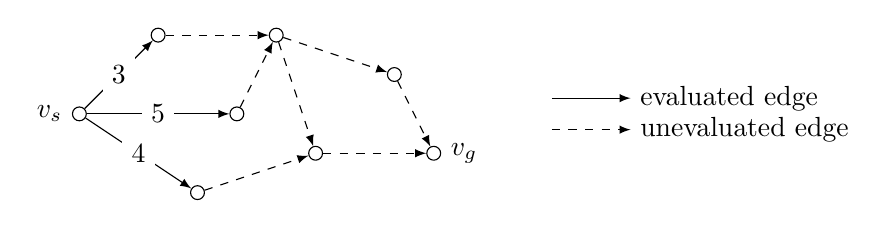
\begin{tikzpicture}
\tikzstyle{vertex}=[circle,draw=black,inner sep=0pt,minimum size=5pt]

\node[vertex] (a) at (0,0) {};
\node[vertex] (b) at (2,0) {};
\node[vertex] (c) at (2.5,1) {};
\node[vertex] (d) at (1,1) {};
\node[vertex] (e) at (3,-0.5) {};
\node[vertex] (f) at (4,0.5) {};
\node[vertex] (g) at (4.5,-0.5) {};
\node[vertex] (h) at (1.5,-1) {};

\draw[black,->,>=latex] (a) -- (b) node [midway, fill=white] {5};
\draw[black,->,>=latex] (a) -- (h) node [midway, fill=white] {4};
\draw[black,->,>=latex] (a) -- (d) node [midway, fill=white] {3};
\draw[black,->,dashed,>=latex] (b) -- (c);
\draw[black,->,dashed,>=latex] (d) -- (c);
\draw[black,->,dashed,>=latex] (c) -- (e);
\draw[black,->,dashed,>=latex] (c) -- (f);
\draw[black,->,dashed,>=latex] (f) -- (g);
\draw[black,->,dashed,>=latex] (e) -- (g);
\draw[black,->,dashed,>=latex] (h) -- (e);

\draw[black,->,>=latex] (6,0.2) -- (7,0.2);
\node[anchor=west] at (7,0.2) {evaluated edge};
\draw[black,->,dashed,>=latex] (6,-0.2) -- (7,-0.2);
\node[anchor=west] at (7,-0.2) {unevaluated edge};

\node[left=0pt of a] {$v_s$};
\node[right=0pt of g] {$v_g$};

\end{tikzpicture}
\caption{A small explicit graph with some evaluated edges.}
\label{fig:seg-intro}
\end{figure}

\subsection{Generic Best-First Search Algorithm over Paths}

Best-first search \cite{winston1977ai}
is a general class of search algorithms.
We choose to express the general algorith
over \emph{paths} instead of \emph{vertices}
for clarity and generality
because we are focused primarily on explicit graphs.
However, Section~\ref{sec:implicit} shows
how it reduces to traditional A* search
for certain types of evaluation functions,
as is required when searching over implicit graphs.

\begin{algorithm}
\caption{Generic Best-First Search Algorithm}
\label{alg:generic-best-first}
\begin{algorithmic}[1]
\Procedure {\textsc{GenericBestFirst}}{$G$}
\Loop
   \State $\pi^* = \arg \min\limits_{\Pi} f(\pi)$
      \Comment{For some path cost function $f(\pi)$}
      \label{line:select-optimistic-path}
   \If {$\pi^*$ fully evaluated}
      \State \Return $\pi^*$
   \EndIf
   \State \textsc{Evaluate}$(\pi^*)$
      \Comment{For some evaluate function}
\EndLoop
\EndProcedure
\end{algorithmic}
\end{algorithm}

Consider the general best-first search algorithm
(Algorithm~\ref{alg:generic-best-first}).
It maintains some sort of data structure storing known data about the
graph (e.g. tags on vertices or edges).
It simply iterates over optimistically-optimal ``best'' paths,
partially evaluating each.
(Note especially the greedy nature of this search.)
See Figure~\ref{fig:seg-edge-example} for a simple example.

\begin{figure}
\centering
\begin{subfigure}[b]{0.45\textwidth}
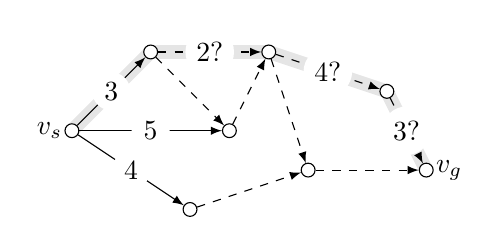
\begin{tikzpicture}
\tikzstyle{vertex}=[circle,draw=black,fill=white,inner sep=0pt,minimum size=5pt]

\coordinate (a) at (0,0);
\coordinate (b) at (2,0);
\coordinate (c) at (2.5,1);
\coordinate (d) at (1,1);
\coordinate (e) at (3,-0.5);
\coordinate (f) at (4,0.5);
\coordinate (g) at (4.5,-0.5);
\coordinate (h) at (1.5,-1);

\draw[black!10,line width=5pt,line cap=round] (a) -- (d) -- (c) -- (f) -- (g);

\node[vertex] (na) at (a) {};
\node[vertex] (nb) at (b) {};
\node[vertex] (nc) at (c) {};
\node[vertex] (nd) at (d) {};
\node[vertex] (ne) at (e) {};
\node[vertex] (nf) at (f) {};
\node[vertex] (ng) at (g) {};
\node[vertex] (nh) at (h) {};

\draw[black,->,>=latex] (na) -- (nb) node [circle,inner sep=2pt,midway,fill=white] {5};
\draw[black,->,>=latex] (na) -- (nh) node [circle,inner sep=2pt,midway,fill=white] {4};
\draw[black,->,>=latex] (na) -- (nd) node [circle,inner sep=2pt,midway,fill=white] {3};
\draw[black,->,dashed,>=latex] (nd) -- (nb);
\draw[black,->,dashed,>=latex] (nb) -- (nc);
\draw[black,->,dashed,>=latex] (nd) -- (nc) node [circle,inner sep=2pt,midway,fill=white] {2?};
\draw[black,->,dashed,>=latex] (nc) -- (ne);
\draw[black,->,dashed,>=latex] (nc) -- (nf) node [circle,inner sep=2pt,midway,fill=white] {4?};
\draw[black,->,dashed,>=latex] (nf) -- (ng) node [circle,inner sep=2pt,midway,fill=white] {3?};
\draw[black,->,dashed,>=latex] (ne) -- (ng);
\draw[black,->,dashed,>=latex] (nh) -- (ne);

\node[left=0pt of a] {$v_s$};
\node[right=0pt of g] {$v_g$};

\end{tikzpicture}
\caption{Select optimistic best path}
\end{subfigure}%
\quad%
\begin{subfigure}[b]{0.45\textwidth}
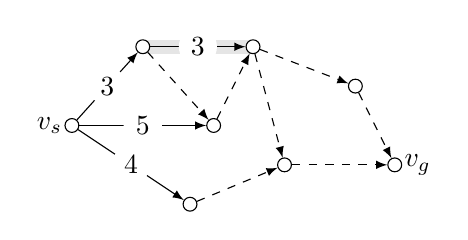
\begin{tikzpicture}
\tikzstyle{vertex}=[circle,draw=black,fill=white,inner sep=0pt,minimum size=5pt]

\coordinate (a) at (0,0);
\coordinate (b) at (1.8,0);
\coordinate (c) at (2.3,1);
\coordinate (d) at (0.9,1);
\coordinate (e) at (2.7,-0.5);
\coordinate (f) at (3.6,0.5);
\coordinate (g) at (4.1,-0.5);
\coordinate (h) at (1.5,-1);

\draw[black!10,line width=5pt,line cap=round] (d) -- (c);

\node[vertex] (na) at (a) {};
\node[vertex] (nb) at (b) {};
\node[vertex] (nc) at (c) {};
\node[vertex] (nd) at (d) {};
\node[vertex] (ne) at (e) {};
\node[vertex] (nf) at (f) {};
\node[vertex] (ng) at (g) {};
\node[vertex] (nh) at (h) {};

\draw[black,->,>=latex] (na) -- (nb) node [circle,inner sep=2pt,midway,fill=white] {5};
\draw[black,->,>=latex] (na) -- (nh) node [circle,inner sep=2pt,midway,fill=white] {4};
\draw[black,->,>=latex] (na) -- (nd) node [circle,inner sep=2pt,midway,fill=white] {3};
\draw[black,->,dashed,>=latex] (nd) -- (nb);
\draw[black,->,dashed,>=latex] (nb) -- (nc);
\draw[black,->,>=latex] (nd) -- (nc) node [circle,inner sep=2pt,midway,fill=white] {3};
\draw[black,->,dashed,>=latex] (nc) -- (ne);
\draw[black,->,dashed,>=latex] (nc) -- (nf);
\draw[black,->,dashed,>=latex] (nf) -- (ng);
\draw[black,->,dashed,>=latex] (ne) -- (ng);
\draw[black,->,dashed,>=latex] (nh) -- (ne);

\node[left=0pt of a] {$v_s$};
\node[right=0pt of g] {$v_g$};

\end{tikzpicture}
\caption{Evaluate first unevaluated edge}
\end{subfigure}%
\caption{Generic best-first algorithm for an explicit graph,
   with $f(\pi)$ best known cost-from-start,
   and {\sc Eval} forward edge evaluations.
   This algorithm is guaranteed to terminate with a feasible path
   with mimimum path cost, if one exists.}
\label{fig:seg-edge-example}
\end{figure}

There are two choices:

\textbf{Cost Function $f(\pi)$.}
What is the cost function $f(\pi)$ over paths used to select the
path for evaluation at each iteration?
For now, we will use the following path objective:
\begin{equation}
   f_x(\pi) = \mbox{\emph{optimistic estimate of execution effort}}.
\end{equation}
In other worts, $f_x(\pi)$ gives a lower bound on the cost of executing
path $p$.
If the path consists of a mix of evaluated and unevaluated edges,
we could write this as:
\begin{equation}
   f_x(\pi) = \sum_{e \in \pi} \left\{
   \begin{array}{cl}
      c[e] & \mbox{if edge } e \mbox{ evaluated}  \\
      \hat{c}(e) & \mbox{otherwise} \\
   \end{array}
   \right.
   .
   \label{eqn:execution-cost-objective}
\end{equation}

\textbf{{\sc Evaluate} Procedure.}
How is a potential path evaluated?

The choice of these two components of the algorithm depend on what
functions are defined over the graph.
Likewise, the data structure is dependent on what is required
for the choices.

\subsection{Best-First Search on Implicit Graphs}
\label{sec:implicit}

Figure~\ref{fig:seg-edge-example} searches an explicit graph,
in which the entire graph structure is represented in memory.
Here, we briefly relate this path-oriented treatment of graph search
to well-known existing algorithms.

Often, due to resource constraints or convenience,
the graph is instead expressed \emph{implicitly}
with one or more operators which calculate the structure of the graph
in the local vicinity of a given vertex.
Initialized with one or more vertices (e.g. starts and/or goals),
an algorithm can incrementally ``discover'' more of the implicit
graph by repeatedly calling such function on discovered vertices.
As a result of this representation,
only a small portion of the graph might need to be explored
during the search.

Due to this implicit representation,
it is clear that each candidate path in $\Pi$ to be considered
(line \ref{line:select-optimistic-path})
cannot generally exist of entirely known edges.
When enumerating candidate paths to the goal,
we must include potential ``virtual'' path segments
through the as-yet undiscovered portion of the graph
to approximate the path cost function $f(\pi)$.
The behavior of the search depends on this approximation,
as well as the nature of {\sc Evaluate} function induced by
the implicit representation operator(s) available.
Several variants are briefly discussed here.

\subsubsection{Relation to A*}

The most common implicit graph representation
is the \emph{expansion} or \emph{successor} function {\sc Successors}$(v)$
which yields all vertices reachable from the parent vertex $v$,
along with the associated edge costs.

Suppose, for now, that we only consider candidate paths that consist of:
(a) a first segment consisting over zero or more evaluated edges,
followed by
(b) an unexpanded ``frontier'' vertex $v_f$, followed by
(b) a second segment through the undiscovered portion of the graph.
We can then express $f_x(\pi)$ as:
\begin{equation}
   f_x(\pi)
   = \underbrace{f_{s \rightarrow v_f}(\pi)}_{g[v_f]}
   + \underbrace{f_{v_f \rightarrow g}(\pi)}_{h(v_f)}.
\end{equation}
These components correspond to the best-known cost-to-come $g[v_f]$
and the heuristic function $h(v_f)$ from A* search \cite{hart1968astar}.
See Figure~\ref{fig:seg-implicit} for an example with $h(v_f)=0$.

We can now produce a proof that as long as $h(v_f)$ is admissible,
and we are restricted to an {\sc Eval}$(\pi)$ function which 
expands the first unexpanded vertex,
the optimistic-optimal path $\pi^*$ at each iteration
follows the structure in the previous paragraph.
See Appendix~\ref{appendix:gs-proofs}.

\begin{figure}
\centering
\begin{subfigure}[b]{0.45\textwidth}
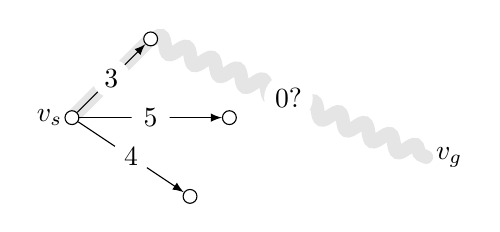
\begin{tikzpicture}
\tikzstyle{vertex}=[circle,draw=black,fill=white,inner sep=0pt,minimum size=5pt]

\coordinate (a) at (0,0);
\coordinate (b) at (2,0);
\coordinate (c) at (2.5,1);
\coordinate (d) at (1,1);
\coordinate (e) at (3,-0.5);
\coordinate (f) at (4,0.5);
\coordinate (g) at (4.5,-0.5);
\coordinate (h) at (1.5,-1);

\draw[black!10,line width=5pt,line cap=round] (a) -- (d);
\draw[black!10,line width=5pt,line cap=round,
   decorate,decoration=snake]
   (d) -- (g) node [black,circle,inner sep=2pt,midway,fill=white] {0?};

\node[vertex] (na) at (a) {};
\node[vertex] (nb) at (b) {};
%\node[vertex] (nc) at (c) {};
\node[vertex] (nd) at (d) {};
%\node[vertex] (ne) at (e) {};
%\node[vertex] (nf) at (f) {};
%\node[vertex] (ng) at (g) {};
\node[vertex] (nh) at (h) {};

\draw[black,->,>=latex] (na) -- (nb) node [circle,inner sep=2pt,midway,fill=white] {5};
\draw[black,->,>=latex] (na) -- (nh) node [circle,inner sep=2pt,midway,fill=white] {4};
\draw[black,->,>=latex] (na) -- (nd) node [circle,inner sep=2pt,midway,fill=white] {3};

\node[left=0pt of a] {$v_s$};
\node[right=0pt of g] {$v_g$};

\end{tikzpicture}
\caption{Select optimistic best path}
\end{subfigure}%
\quad%
\begin{subfigure}[b]{0.45\textwidth}
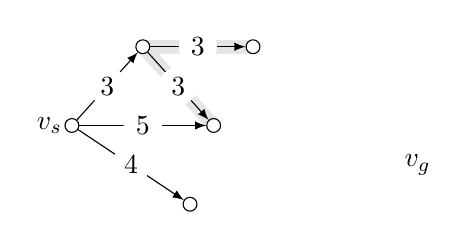
\begin{tikzpicture}
\tikzstyle{vertex}=[circle,draw=black,fill=white,inner sep=0pt,minimum size=5pt]

\coordinate (a) at (0,0);
\coordinate (b) at (1.8,0);
\coordinate (c) at (2.3,1);
\coordinate (d) at (0.9,1);
\coordinate (e) at (2.7,-0.5);
\coordinate (f) at (3.6,0.5);
\coordinate (g) at (4.1,-0.5);
\coordinate (h) at (1.5,-1);

\draw[black!10,line width=5pt,line cap=round] (d) -- (c);
\draw[black!10,line width=5pt,line cap=round] (d) -- (b);

\node[vertex] (na) at (a) {};
\node[vertex] (nb) at (b) {};
\node[vertex] (nc) at (c) {};
\node[vertex] (nd) at (d) {};
%\node[vertex] (ne) at (e) {};
%\node[vertex] (nf) at (f) {};
%\node[vertex] (ng) at (g) {};
\node[vertex] (nh) at (h) {};

\draw[black,->,>=latex] (na) -- (nb) node [circle,inner sep=2pt,midway,fill=white] {5};
\draw[black,->,>=latex] (na) -- (nh) node [circle,inner sep=2pt,midway,fill=white] {4};
\draw[black,->,>=latex] (na) -- (nd) node [circle,inner sep=2pt,midway,fill=white] {3};
\draw[black,->,>=latex] (nd) -- (nb) node [circle,inner sep=2pt,midway,fill=white] {3};
\draw[black,->,>=latex] (nd) -- (nc) node [circle,inner sep=2pt,midway,fill=white] {3};

\node[left=0pt of a] {$v_s$};
\node[right=0pt of g] {$v_g$};

\end{tikzpicture}
\caption{Expand first unexpanded vertex}
\end{subfigure}%
\caption{Best-first algorithm for an implicit graph,
   with $f(\pi)$ best known cost-from-start,
   and {\sc Eval} forward vertex expansions.
   This is Dijkstra's algorithm \cite{dijkstra1959anote}.}
\label{fig:seg-implicit}
\end{figure}

Takeaway: A* uses a general heuristic function $h_g(v)$
because it doesn't have a representation of the full graph,
so it can't compute an actual best optimistic path.
I claim that for manipulation planning problems,
we can indeed reason over explicit graphs.

\subsubsection{Relation to BHFFA}

Let's say that we also have a function which computes the predecessors
of a vertex,
and also an admissible heuristic function $h(v_a,v_b)$ which computes
a lower-bound estimate of the optimal cost between two vertices.
Then the best-first thing to do is equivalent to the
Bidirectional Heuristic Front-to-Front Algorithm \cite{sint1977bhffa}.

\subsection{Best-First Search with Edge Evaluation}

What if, instead of operating over vertices (like A* and the like),
we operate over edges?
Figure~\ref{fig:seg-intro} illustrated the simplest such algorithm,
which selects the optimistic-optimal path,
and then evaluates the first as-yet unevaluated edge on the path.

I think that the forward-evaluation version of this is the same as
Optimal Generation A* (OPA*) and Simple Optimal Generation A* (SOGA*)
\cite{goldenberg2013epeastar},
which are modified versions of
Enhanced Partial Expansion A* \cite{felner2012epastar}.

\subsection{Bidirectional {\sc Eval} Procedures}

In general, over explicit graphs,
it usually makes sense to do bidirectional evaluations.
I need some data to back this up for my problem.
For example,
the Lazy PRM algorithm \cite{bohlin2000lazyprm}
is just best-first search
applied to binary edge cost functions
($c(e) \in \{ \hat{c}(e), \infty \}$)
with bidirectional edge evaluations
(although it actually uses a slightly fancier path evaluation function).

\section{Penalizing Planning Effort}

So far, we've been searching for a path which optimizes our solution
cost objective (\ref{eqn:execution-cost-objective}).
However, as we motivated in the introduction,
there are two distint notions of efficency,
and our objective so far (\ref{eqn:execution-cost-objective})
has only captured one of the two.
Here, we focus instead on \emph{planning efficiency},
and attempt to define an objective which captures it.
We hope that doing so will lead to searches which consume less 
time or energy.

\begin{equation}
   f_p(\pi) = \mbox{\emph{optimistic estimate of planning effort}}.
\end{equation}

What type of metric should we use?

\subsection{Metrics for Planning Effort}

For problems over very large graphs,
planning effort may be dominated by expanding vertices
or maintaining priority queues.
Therefore, traditional metrics for evaluating planning
effort are \emph{vertices expanded}
and \emph{heap percolates}.
However, for many manipulation problems,
search time is instead dominated by edge evaluations.

Therefore, we introduce a new objective $f_p$
which penalizes remaining effort required to evaluate edges
along a potential path:
\begin{equation}
   f_p(\pi) = \sum_{e \in \pi} \left\{
   \begin{array}{cl}
      0 & \mbox{if edge } e \mbox{ evaluated}  \\
      \hat{p}(e) & \mbox{otherwise} \\
   \end{array}
   \right.
   .
\end{equation}
This uses a new heuristic $\hat{p}(e)$ which estimates the cost
associated with evaluating an edge.
This could be planning time, computational energy required, etc.

The first graph planner to explicitly include such a heuristic
to estimate the remaining
computational planning effort in a best-first search
was A$_\epsilon^*$ \cite{pearl1982semiadmissible}.
While the approach we take is different from that of
\cite{pearl1982semiadmissible},
a motivating quote from this paper is relevant:
\begin{quote}
``The heuristic [\,$\hat{c}$\,] ... is of an entirely
different nature than the ... heuristic [\,$\hat{p}$\,] ... .
The former anticipates the reduction in \emph{solution quality} due to the
remaining part of the solution once it is found;
the latter estimates the \emph{computational effort}
required for completing the search.''
\end{quote}

Sidenote: RRT-Connect is sort of explicitly doing this
(optimizing at each step only for planning time,
but constrained to pass through the sampled point).

\subsection{General Weighted Objective}

In general, we might consider weighting each objective:
\begin{equation}
   f(\pi) = \lambda f_p(\pi) + (1 - \lambda) f_x(\pi) .
   \label{eqn:general-objective}
\end{equation}
Note that with $\lambda=0$,
we recover our old solution cost objective $f_x(\pi)$.
Note that this objective is used in an optimistic, greedy fashion at each
iteration of best-first search.

This is the objective used by the Greedy PRM,
described in Section~\ref{sec:greedy-prm}.

When expanded,
this can then be written:
\begin{equation}
   f(\pi) = \sum_{e \in \pi} \left\{
   \begin{array}{cl}
      (1 - \lambda) c[e] & \mbox{if edge } e \mbox{ evaluated}  \\
      \lambda \hat{p}(e) + (1 - \lambda) \hat{c}(e) & \mbox{otherwise} \\
   \end{array}
   \right.
   .
   \label{eqn:general-objective-explicit}
\end{equation}

\subsection{Simplification with Propotional Heuristics}

Suppose that our edge evaluation cost heuristic
were proportional to our edge execution cost heuristic,
\begin{equation}
   \hat{p}(e) = \alpha \, \hat{c}(e) .
\end{equation}
This might happen if, for example, each were proportional to the edge's
\emph{distance} (with longer paths taking longer to both collision check
and execute at constant velocity).
In this case, we can write:
\begin{equation}
   f(\pi) = (1-\lambda) \sum_{e \in \pi} \left\{
   \begin{array}{cl}
      c[e] & \mbox{if edge } e \mbox{ evaluated}  \\
      \left[ 1 + \frac{\alpha\lambda}{1 - \lambda} \right] \hat{c}(e) & \mbox{otherwise} \\
   \end{array}
   \right.
   .
   \label{eqn:prop-heuristics}
\end{equation}

\subsection{Equivalence to Weighted A*}

Consider the case where we're using forward vertex or edge evaluations
(as is required with implicit graph representations),
and $\lambda < 1$.
In this case, we can rewrite (\ref{eqn:prop-heuristics})
simply as:
\begin{equation}
   f(\pi) \propto
   \underbrace{\sum_{e \; \mbox{\scriptsize evaled}} c[e]}_{g[v_f]}
   +
   \underbrace{\left[ 1 + \frac{\alpha \lambda}{1-\lambda} \right]}_{
      \mbox{\scriptsize inflation factor } \epsilon}
   \underbrace{\hat{c}(e_{last})}_{h(v_f)}
   .
\end{equation}

In other words,
\emph{weighted A* is simply best-first search whose objective
   includes a planning effort term.}

In particular, if planning effort is proportional to execution
effort by a factor of $\alpha$,
a weighted A* search with inflation factor $\epsilon$
is the result of best-first search with
$\lambda = \frac{\epsilon-1}{\alpha+\epsilon-1}$.

\subsection{Relation to Experience Graphs}
\label{sec:egraphs}

Experience graphs \cite{phillips2012egraphs}
are a type of best-first search which
are designed to find paths quickly by incentivizing the planner
to rely on on edges from previous successful plans.

While the E-graph planner is originally expressed over implicit graphs,
we can instead express it as best-first search over paths
with the following objective:
\begin{equation}
   f_{\mbox{\scriptsize E-graphs}}(\pi) \propto \sum_{e \in \pi} \left\{
   \begin{array}{cl}
      c[e] & \mbox{if edge } e \mbox{ evaluated, this search} \\
      \epsilon \, c[e] & \mbox{if edge } e \mbox{ evaluated, previous search} \\
     \epsilon \, \epsilon^E \, \hat{c}(e) & \mbox{otherwise} \\
   \end{array}
   \right.
   \label{eqn:prop-heuristics}
\end{equation}

The Greedy PRM applied to a single $C_{free}$ as described in this chapter
is equivalent to the E-Graph planner
with $\epsilon=1$ and $\epsilon^E = 1 + \frac{\alpha \lambda}{1-\lambda}$.
It's not immediately clear to me why one would choose $\epsilon \neq 1$.
(Note: we don't do shortcuts or snap motions.)

\section{Planner: Greedy PRM}
\label{sec:greedy-prm}

The Greedy PRM is the result of applying
best-first search with the $\lambda$-mediated objective
(\ref{eqn:general-objective})
to a simple single-$C_{free}$ problem
in batches of $N$ samples.
Based on empirical results, we also use the bidirectional edge evaluation
algorithn,
since it tends to finish faster.

The Greedy PRM is the result of applying
best-first graph search to
a probabilistic roadmap \cite{kavrakietal1996prm}
embedded in $\mathcal{C}$,
where the cost of each edge captures an optimistic estimate of
the execution cost and the current planning cost remaining.
The planner effectively exploits the multi-set structure
from Section~\ref{subsec:problem-definition},
guided by the cost model from Section~\ref{subsec:cost-model}
to minimize total task cost.

The Greedy PRM is \emph{multi-query},
in that the same graph
structure $G$ is maintained within the configuration space
$\mathcal{C}$.

The algorithm is also \emph{lazy},
in that edge evaluations are deferred until they are needed.
In fact, it can be seen as a generalization of the
LazyPRM \cite{bohlin2000lazyprm}
which also considers planning cost in its objective.
Further,
the algorithm is heuristic-focused,
and its behavior mimics that of an inflated heuristic planner
depending on the selection of the planning/execution cost
tradeoff parameter $\lambda$
as described in Section~\ref{subsec:alg-opt-path-cost}.

\subsection{Best-First Search over Paths on Explicit Graphs}
\label{subsec:alg-greedy-prm}

\begin{algorithm}
\caption{Greedy PRM}
\label{alg:greedy-prm}
\begin{algorithmic}[1]
\Procedure {\textsc{MultiSetPRM}}{$G, \mathcal{Q}, N, \lambda$}
%\State $G.V \leftarrow \emptyset$
%\State $G.E \leftarrow \emptyset$
\Loop
   \State \textsc{PrmAddSamples}($G, \mathcal{Q}, N$)
      \Comment See Sec.~\ref{subsec:alg-greedy-prm}
   \Loop
         \label{line:best-first-start}
      \State $\pi^* = \argmin\limits_{\pi \in \Pi(G,\mathcal{Q})}
         \big[ \lambda \, f_p[\pi] + (1 - \lambda) \, f_e[\pi] \big]$
         \label{line:select-optimistic-path}
      \If {$\pi^* = \mbox{\textbf{nil}}$}
        \State \textbf{break}
      \EndIf
      \If {\textsc{EvalPath}$(\pi^*)$}
         \State \Return $\pi^*$
            \Comment Success
      \EndIf
   \EndLoop
      \label{line:best-first-end}
\EndLoop
\EndProcedure
\end{algorithmic}
\end{algorithm}

The Greedy PRM (Alg.~\ref{alg:greedy-prm})
operates on an initially empty persistent roadmap graph $G$.
Each vertex represents a configuration $x \in \mathcal{C}$,
and each edge represents a path $x(t)$ planned by a local planner.
Similarly to the LazyPRM,
edges are not evaluated until necessary.

The algorithm proceeds in \emph{batches};
at the start of each batch,
the \textsc{PrmAddSamples} procedure adds
$N$ additional vertices to the graph sampled from $\mathcal{C}$
(including sampled start and goal configurations from $\mathcal{Q}$
if not yet present),
and edges are generated according to the PRM construction method.
The Multi-Set PRM does not commit to any particular such method
(e.g. r-disk, K-nearest-neighbors).

The remainder of the algorithm
(lines \ref{line:best-first-start} - \ref{line:best-first-end})
proceeds as a best-first search over paths.
At each iteration,
we select the potentially feasible path $\pi^*$
which minimizes the optimistic
planning/execution cost function.
If no such path exists
(all paths have been shown to be infeasible),
we introduce a new batch.
Otherwise, we evaluate the current path with
\textsc{EvalPath}
(Section~\ref{subsec:alg-path-evaluation}),
returning the path on success.

Note that while
algorithm~\ref{alg:greedy-prm} supposes that you completely solve
one query before moving on to the next,
the planner can be interrupted at any point,
allowing for interleaving queries.

Line~\ref{line:select-optimistic-path}
implements the Greedy PRM's objective
which trades off between planning and execution cost,
mediated by the parameter $\lambda \in [0,1]$.
Adjusting $\lambda$ varies the behavior between feasible and optimal.
With $\lambda = 0$,
only execution cost is considered,
and the algorithm reduces to the LazyPRM
(assuming it's applied to a simple, single-set problem).

The execution cost component is given by $f_e[x(t)]$
as defined in the cost model $\mathcal{M}$
(Section~\ref{subsec:cost-model}).
The optimistic estimate of the remaining planning cost for the path
is computed by determining the cost of the optimistic plan for each
edge using the \textsc{OptEdgePlan} function
(Section~\ref{subsec:alg-opt-edge-plan}).

\subsection{Path Evaluation}
\label{subsec:alg-path-evaluation}

\begin{algorithm}
\caption{Partial Path Evaluation}
\label{alg:path-evaluation}
\begin{algorithmic}[1]
\Function {\textsc{EvalPath}}{$\pi$}
   \ForAll {$e \in \pi$}
         \label{line:edge-evaluation-order}
      \State $(S_{plan}, b_{plan}, c_{plan})
         = \mbox{\textsc{OptEdgePlan}}(e)$
      \ForAll {$X \in S_{plan}$}
         \State $b_{act} = \mathbf{1}_X[e]$
         \State $\arraycolsep=2pt
            e.P \leftarrow e.P \cup
            \left\{\left( \begin{array}{rl}
            \mathbf{1}_X & \mbox{if } b_{act} \\
            \lnot \mathbf{1}_X & \mbox{otherwise} \\
            \end{array} \right)
            \right\}$
         \If {$b_{act} \neq b_{plan}(X)$}
            \State \Return False
         \EndIf
      \EndFor
   \EndFor
   \State \Return True
\EndFunction
\end{algorithmic}
\end{algorithm}

Once a candidate path is selected,
it is evaluated by the \textsc{EvalPath} function
(Alg.~\ref{alg:path-evaluation}).
Line~\ref{line:edge-evaluation-order} iterates over edges in
the path,
which can be done in any order;
see Section~\ref{subsec:implementation-details} for details.
For each edge $e$,
the planned indicator evaluations are actually performed
(this tends to dominate planning costs).
The evaluation proceeds until an evaluation does not succeed.

\subsection{Implementation Details}
\label{subsec:implementation-details}

We provide an implementation of the Multi-Set PRM
as a plugin for the Open Motion Planning Library \cite{sucan2012ompl}.%
\footnote{Not available during the anonymous review process.}
Here, we discuss a few relevant details of the implementation.

We implement the algorithm's best-first search 
(line~\ref{line:best-first-start} of Alg.~\ref{alg:greedy-prm})
using a bidirectional variant of Dijkstra's algorithm
\cite{dijkstra1959anote}.
This requires that the execution cost functional $f_e[x(t)]$
be additive.
Efficiency could be further increased by applying incremental
graph search algorithms \cite{koenig2004lpastar} to the problem.
We implement the indicator functionals $\mathbf{1}_X[x(t)]$
approximately by evaluating the corresponding indicator functions
$\mathbf{1}_X(x)$ at a fixed resolution along the path.

\subsection{Choosing the Execution Cost Functional}

How to represent execution cost?
Ideally, this would be additive.
Sidd wants me to play with Hauser's fast bounded-velocity,
bounded-acceleration segment timing code
(which starts and stops at each waypoint).

\subsection{Choosing $\lambda$}

Minimizing total time in a greedy fashion implies $\lambda = 0.5$.
For later steps in a multi-step plan,
we might have an estimate of the probability $P_e$ that the given query will
actually be executed.
We can then pose our optimistic objective as total planning and execution
time in expection;
this induces the following parameter choice:
\begin{equation}
   \lambda = \frac{1}{1 + P_e} .
\end{equation}
For example, $P_e=1$ induces $\lambda = 0.5$;
as $P_e \rightarrow 0$, $\lambda \rightarrow 1$.
In other words,
as the estimated probability of executing the path goes down,
the planner becomes greedier w.r.t. planning effort at the expense of
costlier solution paths.

This is all one-step greedy;
it returns the optimal path optimistically,
assuming it will be collision-free.
If we have some estimate of the proportion $P_u$ of evaluated edges
which will be part of the final path,
we can then choose a cost function which downweights the planning time.
I need to work this out. 

\subsection{Choosing Batch Size $N$}

\cdnote{Actuall, I think I should move this to
Chapter~\ref{chap:graphs-in-continuous}.}
What graph are we searching over?
If it's too sparse, we'll stop after knowing that no solution exists.
If it's too dense, we'll spend too much time filling in parts of
space.
There's actually some spatial relationship in $C_{free}$ what we're not
modeling.
We get around this with artificial sparseness.
There's definitely a paper's worth of work here too (Shushman's stuff).
The easy version is with sequential batches of size $N$.
Talk about how what we really want to do
is evaluate the estimate of cost remaining
\emph{in expectation}.

Talk about how this is complementary to BIT* which acheive speedups
by batching, not by inflating.

\section{Results}

Here are results.
See Figure~\ref{fig:bean} and Figure~\ref{fig:herb-comparison-cdfs}.

I hope to show that the Greedy PRM is competitive with RRT-Connect
in terms of planning effort required to find a feasible path.

\begin{figure}
\centering
\begin{subfigure}[b]{0.3\textwidth}
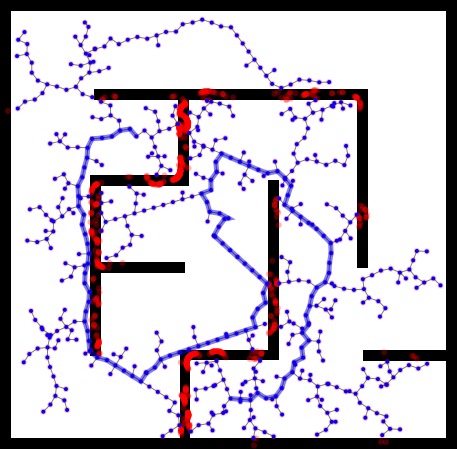
\includegraphics[width=\textwidth]{figs/compare-2d-rrtc1-rrtextcon-r1-s1.png}
\caption{RRT Ext-Con, R=1}
\end{subfigure}%
\quad
\begin{subfigure}[b]{0.3\textwidth}
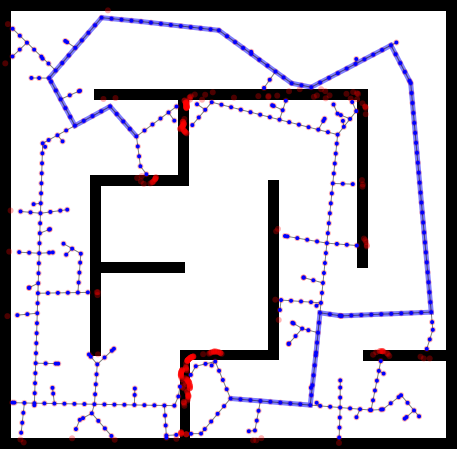
\includegraphics[width=\textwidth]{figs/compare-2d-rrtc1-rrtconcon-r1-s1.png}
\caption{RRT Con-Con, R=1}
\end{subfigure}%
\quad
\begin{subfigure}[b]{0.3\textwidth}
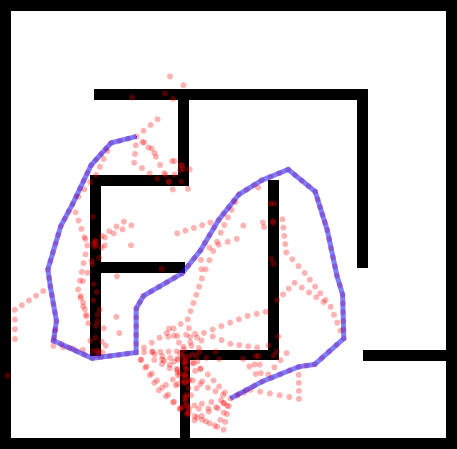
\includegraphics[width=\textwidth]{figs/compare-2d-rrtc1-checkmask-l00-s1.png}
\caption{Greedy PRM, $\lambda=0$}
\end{subfigure}%
\vspace{0.05in}
\begin{subfigure}[b]{0.3\textwidth}
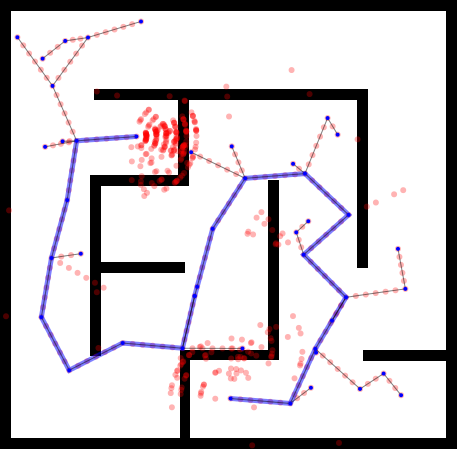
\includegraphics[width=\textwidth]{figs/compare-2d-rrtc1-rrtextcon-r6-s1.png}
\caption{RRT Ext-Con, R=6}
\end{subfigure}%
\quad
\begin{subfigure}[b]{0.3\textwidth}
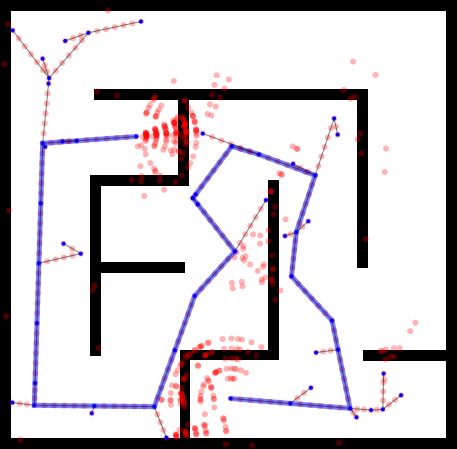
\includegraphics[width=\textwidth]{figs/compare-2d-rrtc1-rrtconcon-r6-s1.png}
\caption{RRT Con-Con, R=6}
\end{subfigure}%
\quad
\begin{subfigure}[b]{0.3\textwidth}
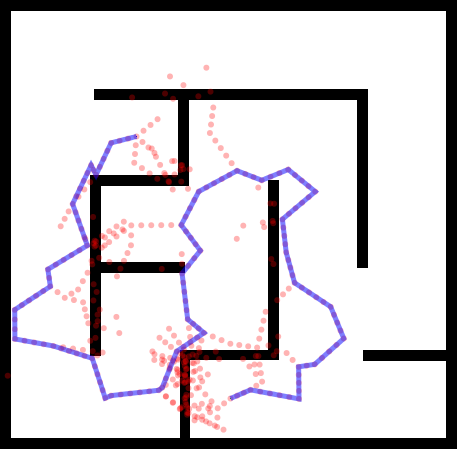
\includegraphics[width=\textwidth]{figs/compare-2d-rrtc1-checkmask-l10-s1.png}
\caption{Greedy PRM, $\lambda=1$}
\end{subfigure}%
\caption{Example runs with different planners,
   with the same sequence of samples.
   Note that Greedy PRM $\lambda=0$ is equivalent to LazyPRM.
   Red dots show collision checks.}
\label{fig:compare-2d-rrtc1-vis}
\end{figure}

\begin{figure}
\centering
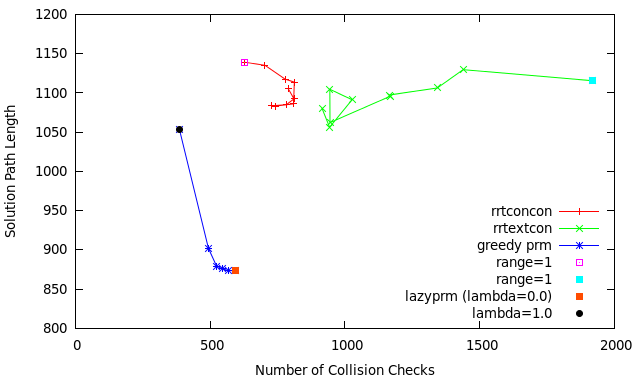
\includegraphics[width=0.8\textwidth]{figs/compare-2d-rrtc1-medians.png}
\caption{Plot of collision checks vs solution path cost for the
   different algorithms from the problem from
   Figure~\ref{fig:compare-2d-rrtc1-vis}.}
\end{figure}

\begin{figure}
\centering
\begin{subfigure}[b]{0.4\textwidth}
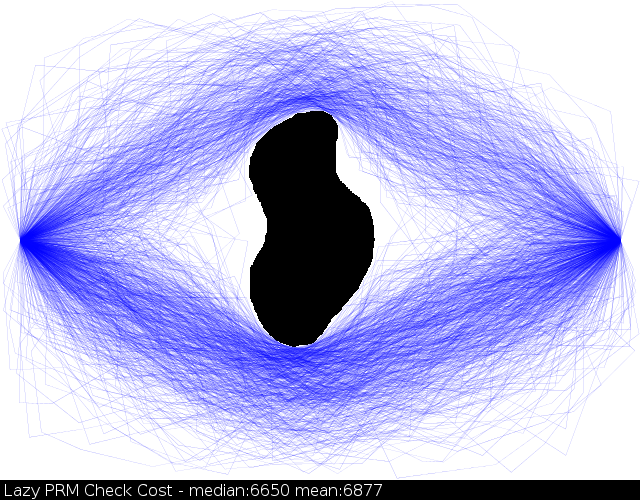
\includegraphics[width=\textwidth]{figs/timegreedy-bean-lambda-00.png}
\caption{Paths with $\lambda = 0$}
\end{subfigure}%
\quad
\begin{subfigure}[b]{0.4\textwidth}
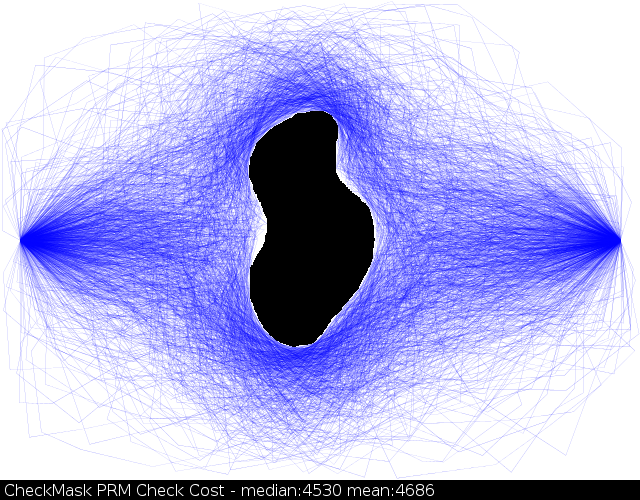
\includegraphics[width=\textwidth]{figs/timegreedy-bean-lambda-10.png}
\caption{Paths with $\lambda = 1$}
\end{subfigure}%
\caption{Examples of paths for a 2d problems
   for different values of $\lambda$.
   As $\lambda$ is increased,
   paths are longer, but are faster to find.}
\label{fig:bean}
\end{figure}

\begin{figure}
\centering
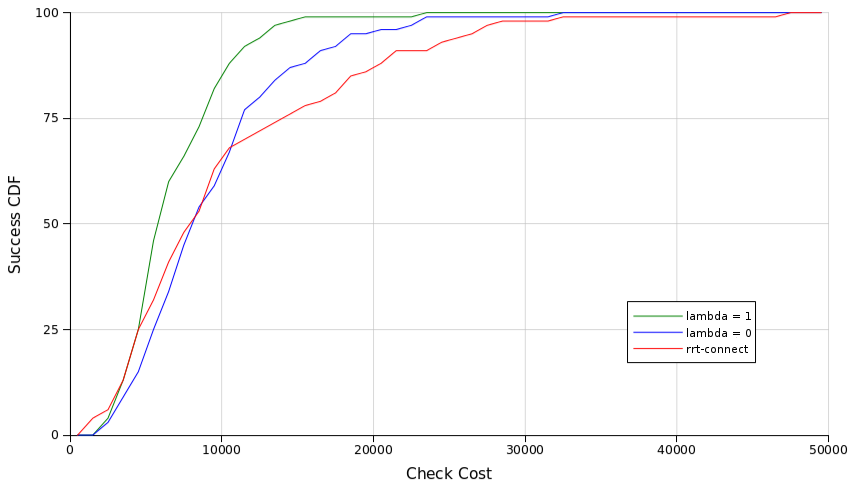
\includegraphics[width=0.8\textwidth]{figs/timegreedy-herbstep1-comparison-cdfs.png}
\caption{Comparison between different algorithms on a HERB problem.
   Must add in ESTs.}
\label{fig:herb-comparison-cdfs}
\end{figure}

\section{Repeated Queries}

For multiple queries within the same $C_{free}$,
the edge evaluations can be used in subsequent searches.
This ends up behaving similarily to E-graphs \cite{phillips2012egraphs}
with $\epsilon=1$
as described in Section~\ref{sec:egraphs},
with the exception that all evaluated edges are placed in the graph,
not just the edges on the solution path.

\section{Constraints}
\label{sec:constraints}

Here I talk about constrained planning.

\section{Future Work}

How to handle the narrow passage problem?
Lots of literature on that, new sampling strategies, etc.
(Toggle PRM, for instance.)


\newpage
\chapter{Roadmaps in Continuous Spaces}
\label{chap:graphs-in-continuous}

Sweet, sweet chapter about how to best embed explicit graphs
in continuous configuration spaces.
Talk about the $N$ parameter.
Extend the Greedy PRM algorith to do things in expectation.
Motivate the incremental densification idea,
with a graduated cost model
to approximate a probabalistic model
of the $\mathcal{C}$-space.
Probabalistic vs lattice-based graphs.

Also talk here about the fancy Lazy PRM path bisection
evaluation function.


\newpage
\chapter{The Multi-Set Planning Problem}
\label{chap:multi-set}

The purpose of this chapter is to introduce the multi-set planning
problem,
talk about its structure in general,
and show how about how a bunch of different problems in manipulation
are instances of this type of problem.

In the introduction to this chapter,
I'll talk about how the multi-step planning problem decomposition
discussed in Chapter~\ref{chap:formulation}
consists of a bunch of different queries in different
$C_{free}$s, but that are related.

For example, say you're planning to move an object from an initial
location to a goal location,
and then move your manipulator back to the start pose.
See Figure~\ref{fig:manip-example}.
You have a single grasp for the object,
and your manipulator has a single IK for the grasp (very simple problem).
There are three $C_{free}$s here;
a naive approach would plan separately in each.

\begin{figure}
\centering
\begin{subfigure}[b]{.45\linewidth}
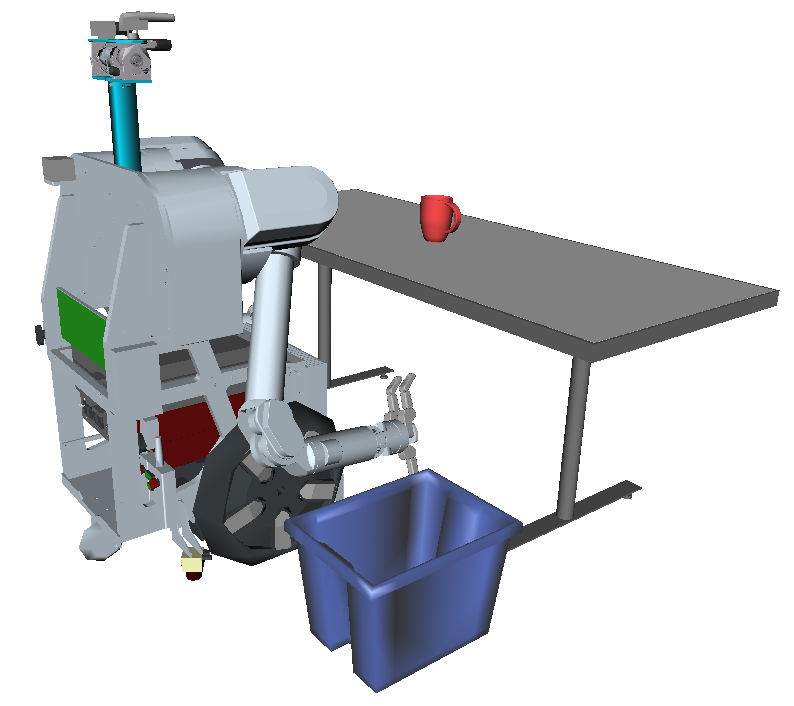
\includegraphics[width=\columnwidth]{figs/simple-table-clearing-task.png}
\end{subfigure}%
\quad%
\begin{subfigure}[b]{.45\linewidth}
\documentclass{standalone}
\usepackage{tikz}
\usetikzlibrary{calc}
\begin{document}
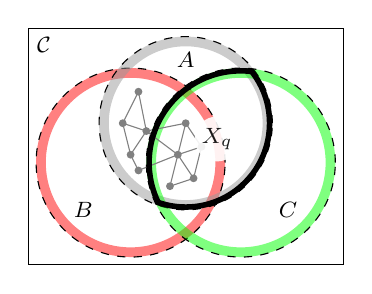
\begin{tikzpicture}

\tikzstyle{every node}=[font=\footnotesize]

\draw (0,0) rectangle (4.0,3.0);

\coordinate (a) at (2.0,1.8);
\coordinate (b) at (1.3,1.3);
\coordinate (c) at (2.7,1.3);

\def\circlea{(a) circle (1.1)}
\def\circleb{(b) circle (1.2)}
\def\circlec{(c) circle (1.2)}

% underlying sets
\begin{scope}
   \clip \circleb;
   \draw[color=red!50,line width=7pt] \circleb;
\end{scope}
\draw[dashed] \circleb;

\begin{scope}
   \clip \circlea;
   \draw[color=black!40,opacity=0.5,line width=7pt] \circlea;
\end{scope}
\draw[dashed] \circlea;

\begin{scope}
   \clip \circlec;
   \draw[color=green,opacity=0.5,line width=7pt] \circlec;
\end{scope}
\draw[dashed] \circlec;

% roadmap
\coordinate (v01) at ($ (a) + ( 0.0, 0.0) $);
\coordinate (v02) at ($ (a) + (-0.1,-0.4) $);
\coordinate (v03) at ($ (a) + ( 0.1,-0.7) $);
\coordinate (v04) at ($ (a) + (-0.2,-0.8) $);
\coordinate (v05) at ($ (a) + (-0.6,-0.6) $);
\coordinate (v06) at ($ (a) + (-0.7,-0.4) $);
\coordinate (v07) at ($ (a) + (-0.5,-0.1) $);
\coordinate (v08) at ($ (a) + ( 0.2,-0.3) $);
\coordinate (v09) at ($ (a) + (-0.8, 0.0) $);
\coordinate (v10) at ($ (a) + (-0.6, 0.4) $);
\node[circle,fill=black!50,inner sep=1.0] at (v01) {};
\node[circle,fill=black!50,inner sep=1.0] at (v02) {};
\node[circle,fill=black!50,inner sep=1.0] at (v03) {};
\node[circle,fill=black!50,inner sep=1.0] at (v04) {};
\node[circle,fill=black!50,inner sep=1.0] at (v05) {};
\node[circle,fill=black!50,inner sep=1.0] at (v06) {};
\node[circle,fill=black!50,inner sep=1.0] at (v07) {};
\node[circle,fill=black!50,inner sep=1.0] at (v08) {};
\node[circle,fill=black!50,inner sep=1.0] at (v09) {};
\node[circle,fill=black!50,inner sep=1.0] at (v10) {};
\draw[color=black!50]
   (v01) -- (v02) -- (v03) -- (v04) -- (v02) -- (v05) -- (v06)
   -- (v07) -- (v02) -- (v08);
\draw[color=black!50] (v03) -- (v08) -- (v01) -- (v07);
\draw[color=black!50] (v06) -- (v09) -- (v07) -- (v10) -- (v09);

% AnC
\begin{scope}
   \clip \circlea;
   \clip \circlec;
   \draw[line width=4pt] \circlea;
   \draw[line width=4pt] \circlec;
\end{scope}

\node at (0.2,2.8) {$\mathcal{C}$};
\node at ($ (a) + (0,0.8) $) {$A$};
\node at ($ (b) + (-0.6,-0.6) $) {$B$};
\node at ($ (c) + ( 0.6,-0.6) $) {$C$};

\node[circle,inner sep=1pt,fill=white,fill opacity=0.9]
  at (2.4,1.6) {$X_q$};

\end{tikzpicture}%
\end{document}

\end{subfigure}
\caption{
  The set of valid configurations for an articulated robot (left)
  changes often,
  especially in dynamic environments
  and multi-step manipulation problems.
  By describing this structure explicitly as set relations (right)
  and performing best-first search
  minimizing both planning and execution cost,
  we effectively reuse computation between similar
  problems.}
\label{fig:manip-example}
\end{figure}

\section{From RSS Intro}

Motion planning approaches that build graphs
in the collision-free subset of
\emph{configuration space} \cite{lozanoperez1983cspace},
e.g. the
PRM \cite{kavrakietal1996prm}
and RRT \cite{lavallekuffner1999rrt},
have proven promising
for high-dimensional articulated robotics problems
in unstructured environments.
These approaches devote a large amount of computational effort
testing configurations and paths for collision,
and the resulting graph can then be reused
for other queries in the same collision-free subset.

However,
for manipuation problems,
this subset of the robot's configuration space
is sensitive to the locations and shapes of
both people and objects in the environment,
as well as the robot itself.
In addition, it depends on the shape and pose of any object
grasped by the robot.
This makes it difficult not only to apply the results of prior
planning computation to the current problem,
but also to efficiently consider planned or hypothesized motions,
since we must reconstruct our graph from scratch whenever
the environment changes.
This is especially the case for
multi-step manipulation tasks that must be planned into the future.
%We want to continuously update our representation for detours.

A large body of prior work has focused on methods to
improve planning efficiency on manipulation problems,
which we review in Section~\ref{sec:related-work}.
Our first key insight is that many of these approaches are
in fact special instances of a more general structure,
which we formulate as the \emph{multi-set planning problem}
in Section~\ref{sec:multi-set}.

The Multi-Set PRM,
when applied to manipulation problems,
naturally produces an array of efficient behavior.
Section~\ref{sec:in-manipulation} outlines several such instances,
and also provides selected experimental results
on a multi-step manipulation task.
We also provide an open-source implementation of our algorithm.

\section{Motivation}

Imagine a simple ``pick and place'' manipulation planning scenario
in which an articulated robot in a novel cluttered environment
is tasked with moving a particular object from a start pose to a goal
pose in the scene.

\begin{figure}
\centering
\begin{subfigure}[b]{0.3\textwidth}
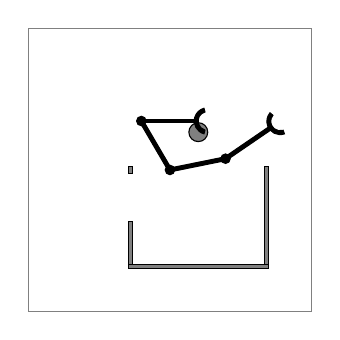
\begin{tikzpicture}
\begin{scope}[scale=1.2]
% bounding rect
\draw[color=black!50, thin] (-1.5,-1.5) rectangle (1.5,1.5);
\tikzstyle{dstyle}=[draw=black,fill=black!50]
\draw[dstyle] (0.300000,0.400000) circle (0.100000);
\draw[dstyle, shift={(0.300000,-1.020000)}, rotate=0.000000] (-0.740000,-0.020000) rectangle (0.740000,0.020000);
\draw[dstyle, shift={(1.020000,-0.480000)}, rotate=0.000000] (-0.020000,-0.520000) rectangle (0.020000,0.520000);
\draw[dstyle, shift={(-0.420000,-0.775000)}, rotate=0.000000] (-0.020000,-0.225000) rectangle (0.020000,0.225000);
\draw[dstyle, shift={(-0.420000,0.000000)}, rotate=0.000000] (-0.020000,-0.040000) rectangle (0.020000,0.040000);

\tikzstyle{dstyle}=[draw=black,fill=black]
\draw[dstyle] (0.000000,0.000000) circle (0.050000);
\draw[dstyle, shift={(0.294020,0.059601)}, rotate=11.459156] (-0.300000,-0.020000) rectangle (0.300000,0.020000);
\draw[dstyle] (0.588040,0.119202) circle (0.050000);
\draw[dstyle, shift={(1.165775,0.514451)}, rotate=214.377468](-74.484513:0.100000) arc (-74.484513:74.484513:0.100000) --(74.484513:0.140000) arc (74.484513:-74.484513:0.140000) -- cycle;
\draw[dstyle, shift={(0.835641,0.288594)}, rotate=34.377468] (-0.300000,-0.020000) rectangle (0.300000,0.020000);

%\tikzstyle{dstyle}=[draw=black!50]
%\draw[dstyle] (0.000000,0.000000) circle (0.050000);
\draw[dstyle, shift={(-0.151454,0.258963)}, rotate=120.321137] (-0.300000,-0.020000) rectangle (0.300000,0.020000);
\draw[dstyle] (-0.302908,0.517926) circle (0.050000);
\draw[dstyle, shift={(0.397092,0.517926)}, rotate=180.000000](-74.484513:0.100000) arc (-74.484513:74.484513:0.100000) --(74.484513:0.140000) arc (74.484513:-74.484513:0.140000) -- cycle;
\draw[dstyle, shift={(-0.002908,0.517926)}, rotate=0.000000] (-0.300000,-0.020000) rectangle (0.300000,0.020000);

\end{scope}
\end{tikzpicture}
\caption{Valid configuration}
\end{subfigure}%
\quad%
\begin{subfigure}[b]{0.3\textwidth}
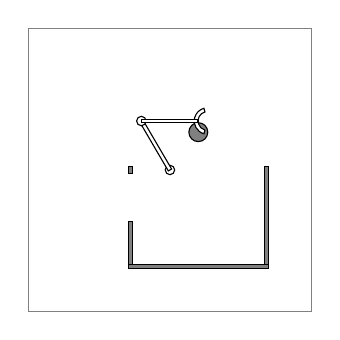
\begin{tikzpicture}
\begin{scope}[scale=1.2]
% bounding rect
\draw[color=black!50, thin] (-1.5,-1.5) rectangle (1.5,1.5);
\tikzstyle{dstyle}=[draw=black,fill=black!50]
\draw[dstyle] (0.300000,0.400000) circle (0.100000);
\draw[dstyle, shift={(0.300000,-1.020000)}, rotate=0.000000] (-0.740000,-0.020000) rectangle (0.740000,0.020000);
\draw[dstyle, shift={(1.020000,-0.480000)}, rotate=0.000000] (-0.020000,-0.520000) rectangle (0.020000,0.520000);
\draw[dstyle, shift={(-0.420000,-0.775000)}, rotate=0.000000] (-0.020000,-0.225000) rectangle (0.020000,0.225000);
\draw[dstyle, shift={(-0.420000,0.000000)}, rotate=0.000000] (-0.020000,-0.040000) rectangle (0.020000,0.040000);

\tikzstyle{dstyle}=[draw=black,fill=white]
\draw[dstyle] (0.000000,0.000000) circle (0.050000);
\draw[dstyle, shift={(-0.151454,0.258963)}, rotate=120.321137] (-0.300000,-0.020000) rectangle (0.300000,0.020000);
\draw[dstyle] (-0.302908,0.517926) circle (0.050000);
\draw[dstyle, shift={(0.397092,0.517926)}, rotate=180.000000](-74.484513:0.100000) arc (-74.484513:74.484513:0.100000) --(74.484513:0.140000) arc (74.484513:-74.484513:0.140000) -- cycle;
\draw[dstyle, shift={(-0.002908,0.517926)}, rotate=0.000000] (-0.300000,-0.020000) rectangle (0.300000,0.020000);

\end{scope}
\end{tikzpicture}
\caption{Invalid configuration}
\end{subfigure}%
\quad%
\begin{subfigure}[b]{0.3\textwidth}
\begin{tikzpicture}
\begin{scope}[scale=0.35]

\tikzstyle{every node}=[font=\scriptsize]

% x,y axes
\draw[->] (-3.14,-3.14) -- (4,-3.14) node[anchor=west] {$\theta_1$};
\draw[->] (-3.14,-3.14) -- (-3.14,4) node[anchor=south] {$\theta_2$};

% x tick marks with labels
\draw[-] (-3.14,-3.4) -- (-3.14,-3.14);
\draw[-] (    0,-3.4) -- (    0,-3.14);
\draw[-] ( 3.14,-3.4) -- ( 3.14,-3.14);
\draw	(-3.14,-3.4) node[anchor=north] {$-\pi$};
\draw	(    0,-3.4) node[anchor=north] {$0$};
\draw	( 3.14,-3.4) node[anchor=north] {$\pi$};

% y tick marks with labels
\draw[-] (-3.4,-3.14) -- (-3.14,-3.14);
\draw[-] (-3.4,    0) -- (-3.14,    0);
\draw[-] (-3.4, 3.14) -- (-3.14, 3.14);
\draw	(-3.4,-3.14) node[anchor=east] {$-\pi$};
\draw	(-3.4,    0) node[anchor=east] {$0$};
\draw	(-3.4, 3.14) node[anchor=east] {$\pi$};

% points
\draw[-,style=dotted] (0.2,-3.14) -- (0.2,0.4) -- (-3.14,0.4);
\draw[fill=black] (0.2,0.4) circle (0.15);
\draw[-,style=dotted] (2.1,-3.14) -- (2.1,-2.1) -- (-3.14,-2.1);
\draw[draw=black,fill=white] (2.1,-2.1) circle (0.15);

% legend
\draw[fill=black] (1,3.2) circle (0.15);
\draw	(1,3.2) node[anchor=west] {valid};
\draw[draw=black,fill=white] (1,2.3) circle (0.15);
\draw	(1,2.3) node[anchor=west] {invalid};

\end{scope}
\end{tikzpicture}
\caption{Configuration space}
\end{subfigure}
\caption{A simple planar 2-link manipulator problem.}
\end{figure}


\begin{figure}
\centering
\begin{subfigure}[b]{0.3\textwidth}
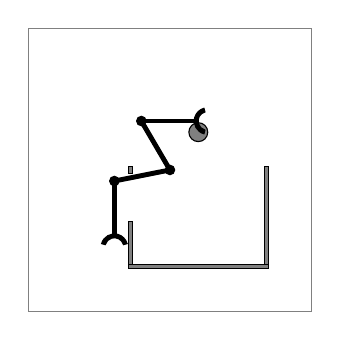
\begin{tikzpicture}
\begin{scope}[scale=1.2]
% bounding rect
\draw[color=black!50, thin] (-1.5,-1.5) rectangle (1.5,1.5);
\tikzstyle{dstyle}=[draw=black,fill=black!50]
\draw[dstyle] (0.300000,0.400000) circle (0.100000);
\draw[dstyle, shift={(0.300000,-1.020000)}, rotate=0.000000] (-0.740000,-0.020000) rectangle (0.740000,0.020000);
\draw[dstyle, shift={(1.020000,-0.480000)}, rotate=0.000000] (-0.020000,-0.520000) rectangle (0.020000,0.520000);
\draw[dstyle, shift={(-0.420000,-0.775000)}, rotate=0.000000] (-0.020000,-0.225000) rectangle (0.020000,0.225000);
\draw[dstyle, shift={(-0.420000,0.000000)}, rotate=0.000000] (-0.020000,-0.040000) rectangle (0.020000,0.040000);

\tikzstyle{dstyle}=[draw=black,fill=black]
\draw[dstyle] (0.000000,0.000000) circle (0.050000);
\draw[dstyle, shift={(-0.294233,-0.058540)}, rotate=-168.747530] (-0.300000,-0.020000) rectangle (0.300000,0.020000);
\draw[dstyle] (-0.588466,-0.117080) circle (0.050000);
\draw[dstyle, shift={(-0.588469,-0.817080)}, rotate=89.999790](-74.484513:0.100000) arc (-74.484513:74.484513:0.100000) --(74.484513:0.140000) arc (74.484513:-74.484513:0.140000) -- cycle;
\draw[dstyle, shift={(-0.588467,-0.417080)}, rotate=-90.000210] (-0.300000,-0.020000) rectangle (0.300000,0.020000);

%\tikzstyle{dstyle}=[draw=black!50]
%\draw[dstyle] (0.000000,0.000000) circle (0.050000);
\draw[dstyle, shift={(-0.151454,0.258963)}, rotate=120.321137] (-0.300000,-0.020000) rectangle (0.300000,0.020000);
\draw[dstyle] (-0.302908,0.517926) circle (0.050000);
\draw[dstyle, shift={(0.397092,0.517926)}, rotate=180.000000](-74.484513:0.100000) arc (-74.484513:74.484513:0.100000) --(74.484513:0.140000) arc (74.484513:-74.484513:0.140000) -- cycle;
\draw[dstyle, shift={(-0.002908,0.517926)}, rotate=0.000000] (-0.300000,-0.020000) rectangle (0.300000,0.020000);

\end{scope}
\end{tikzpicture}
\caption{Valid configuration}
\end{subfigure}%
\quad%
\begin{subfigure}[b]{0.3\textwidth}
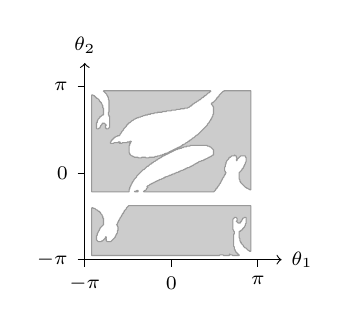
\begin{tikzpicture}
\begin{scope}[scale=0.35]

\tikzstyle{every node}=[font=\scriptsize]

% x,y axes
\draw[->] (-3.14,-3.14) -- (4,-3.14) node[anchor=west] {$\theta_1$};
\draw[->] (-3.14,-3.14) -- (-3.14,4) node[anchor=south] {$\theta_2$};

% x tick marks with labels
\draw[-] (-3.14,-3.4) -- (-3.14,-3.14);
\draw[-] (    0,-3.4) -- (    0,-3.14);
\draw[-] ( 3.14,-3.4) -- ( 3.14,-3.14);
\draw	(-3.14,-3.4) node[anchor=north] {$-\pi$};
\draw	(    0,-3.4) node[anchor=north] {$0$};
\draw	( 3.14,-3.4) node[anchor=north] {$\pi$};

% y tick marks with labels
\draw[-] (-3.4,-3.14) -- (-3.14,-3.14);
\draw[-] (-3.4,    0) -- (-3.14,    0);
\draw[-] (-3.4, 3.14) -- (-3.14, 3.14);
\draw	(-3.4,-3.14) node[anchor=east] {$-\pi$};
\draw	(-3.4,    0) node[anchor=east] {$0$};
\draw	(-3.4, 3.14) node[anchor=east] {$\pi$};

\begin{scope}[shift={(-3.14,-3.14)},scale=6.28]
\tikzstyle{fdstyle}=[color=black!40, fill=black!20, thin]
\filldraw[fdstyle, even odd rule]
   (0.254000,0.312000) -- (0.258000,0.312000) -- (0.262000,0.312000) -- (0.266000,0.312000) -- (0.270000,0.312000) -- (0.274000,0.312000) -- (0.278000,0.312000) -- (0.282000,0.312000) -- (0.286000,0.312000) -- (0.290000,0.312000) -- (0.294000,0.312000) -- (0.298000,0.312000) -- (0.302000,0.312000) -- (0.306000,0.312000) -- (0.310000,0.312000) -- (0.314000,0.312000) -- (0.318000,0.312000) -- (0.322000,0.312000) -- (0.326000,0.312000) -- (0.330000,0.312000) -- (0.334000,0.312000) -- (0.338000,0.312000) -- (0.342000,0.312000) -- (0.346000,0.312000) -- (0.350000,0.312000) -- (0.354000,0.312000) -- (0.358000,0.312000) -- (0.362000,0.312000) -- (0.366000,0.312000) -- (0.370000,0.312000) -- (0.374000,0.312000) -- (0.378000,0.312000) -- (0.382000,0.312000) -- (0.386000,0.312000) -- (0.390000,0.312000) -- (0.394000,0.312000) -- (0.398000,0.312000) -- (0.402000,0.312000) -- (0.406000,0.312000) -- (0.410000,0.312000) -- (0.414000,0.312000) -- (0.418000,0.312000) -- (0.422000,0.312000) -- (0.426000,0.312000) -- (0.430000,0.312000) -- (0.434000,0.312000) -- (0.438000,0.312000) -- (0.442000,0.312000) -- (0.446000,0.312000) -- (0.450000,0.312000) -- (0.454000,0.312000) -- (0.458000,0.312000) -- (0.462000,0.312000) -- (0.466000,0.312000) -- (0.470000,0.312000) -- (0.474000,0.312000) -- (0.478000,0.312000) -- (0.482000,0.312000) -- (0.486000,0.312000) -- (0.490000,0.312000) -- (0.494000,0.312000) -- (0.498000,0.312000) -- (0.502000,0.312000) -- (0.506000,0.312000) -- (0.510000,0.312000) -- (0.514000,0.312000) -- (0.518000,0.312000) -- (0.522000,0.312000) -- (0.526000,0.312000) -- (0.530000,0.312000) -- (0.534000,0.312000) -- (0.538000,0.312000) -- (0.542000,0.312000) -- (0.546000,0.312000) -- (0.550000,0.312000) -- (0.554000,0.312000) -- (0.558000,0.312000) -- (0.562000,0.312000) -- (0.566000,0.312000) -- (0.570000,0.312000) -- (0.574000,0.312000) -- (0.578000,0.312000) -- (0.582000,0.312000) -- (0.586000,0.312000) -- (0.590000,0.312000) -- (0.594000,0.312000) -- (0.598000,0.312000) -- (0.602000,0.312000) -- (0.606000,0.312000) -- (0.610000,0.312000) -- (0.614000,0.312000) -- (0.618000,0.312000) -- (0.622000,0.312000) -- (0.626000,0.312000) -- (0.630000,0.312000) -- (0.634000,0.312000) -- (0.638000,0.312000) -- (0.642000,0.312000) -- (0.646000,0.312000) -- (0.650000,0.312000) -- (0.654000,0.312000) -- (0.658000,0.312000) -- (0.662000,0.312000) -- (0.666000,0.312000) -- (0.670000,0.312000) -- (0.674000,0.312000) -- (0.678000,0.312000) -- (0.682000,0.312000) -- (0.686000,0.312000) -- (0.690000,0.312000) -- (0.694000,0.312000) -- (0.698000,0.312000) -- (0.702000,0.312000) -- (0.706000,0.312000) -- (0.710000,0.312000) -- (0.714000,0.312000) -- (0.718000,0.312000) -- (0.722000,0.312000) -- (0.726000,0.312000) -- (0.730000,0.312000) -- (0.734000,0.312000) -- (0.738000,0.312000) -- (0.742000,0.312000) -- (0.746000,0.312000) -- (0.750000,0.312000) -- (0.754000,0.312000) -- (0.758000,0.312000) -- (0.762000,0.312000) -- (0.766000,0.312000) -- (0.770000,0.312000) -- (0.774000,0.312000) -- (0.778000,0.312000) -- (0.782000,0.312000) -- (0.786000,0.312000) -- (0.790000,0.312000) -- (0.794000,0.312000) -- (0.798000,0.312000) -- (0.802000,0.312000) -- (0.806000,0.312000) -- (0.810000,0.312000) -- (0.814000,0.312000) -- (0.818000,0.312000) -- (0.822000,0.312000) -- (0.826000,0.312000) -- (0.830000,0.312000) -- (0.834000,0.312000) -- (0.838000,0.312000) -- (0.842000,0.312000) -- (0.846000,0.312000) -- (0.850000,0.312000) -- (0.854000,0.312000) -- (0.858000,0.312000) -- (0.862000,0.312000) -- (0.866000,0.312000) -- (0.870000,0.312000) -- (0.874000,0.312000) -- (0.878000,0.312000) -- (0.882000,0.312000) -- (0.886000,0.312000) -- (0.890000,0.312000) -- (0.894000,0.312000) -- (0.898000,0.312000) -- (0.902000,0.312000) -- (0.906000,0.312000) -- (0.910000,0.312000) -- (0.914000,0.312000) -- (0.918000,0.312000) -- (0.922000,0.312000) -- (0.926000,0.312000) -- (0.930000,0.312000) -- (0.934000,0.312000) -- (0.938000,0.312000) -- (0.942000,0.312000) -- (0.946000,0.312000) -- (0.950000,0.312000) -- (0.954000,0.312000) -- (0.958000,0.312000) -- (0.960000,0.310000) -- (0.960000,0.306000) -- (0.960000,0.302000) -- (0.960000,0.298000) -- (0.960000,0.294000) -- (0.960000,0.290000) -- (0.960000,0.286000) -- (0.960000,0.282000) -- (0.960000,0.278000) -- (0.960000,0.274000) -- (0.960000,0.270000) -- (0.960000,0.266000) -- (0.960000,0.262000) -- (0.960000,0.258000) -- (0.960000,0.254000) -- (0.960000,0.250000) -- (0.960000,0.246000) -- (0.960000,0.242000) -- (0.960000,0.238000) -- (0.960000,0.234000) -- (0.960000,0.230000) -- (0.960000,0.226000) -- (0.960000,0.222000) -- (0.960000,0.218000) -- (0.960000,0.214000) -- (0.960000,0.210000) -- (0.960000,0.206000) -- (0.960000,0.202000) -- (0.960000,0.198000) -- (0.960000,0.194000) -- (0.960000,0.190000) -- (0.960000,0.186000) -- (0.960000,0.182000) -- (0.960000,0.178000) -- (0.960000,0.174000) -- (0.960000,0.170000) -- (0.960000,0.166000) -- (0.960000,0.162000) -- (0.960000,0.158000) -- (0.960000,0.154000) -- (0.960000,0.150000) -- (0.960000,0.146000) -- (0.960000,0.142000) -- (0.960000,0.138000) -- (0.960000,0.134000) -- (0.960000,0.130000) -- (0.960000,0.126000) -- (0.960000,0.122000) -- (0.960000,0.118000) -- (0.960000,0.114000) -- (0.960000,0.110000) -- (0.960000,0.106000) -- (0.960000,0.102000) -- (0.960000,0.098000) -- (0.960000,0.094000) -- (0.960000,0.090000) -- (0.960000,0.086000) -- (0.960000,0.082000) -- (0.960000,0.078000) -- (0.960000,0.074000) -- (0.960000,0.070000) -- (0.960000,0.066000) -- (0.960000,0.062000) -- (0.960000,0.058000) -- (0.960000,0.054000) -- (0.960000,0.050000) -- (0.958000,0.048000) -- (0.954000,0.048000) -- (0.952000,0.050000) -- (0.950000,0.052000) -- (0.946000,0.052000) -- (0.944000,0.054000) -- (0.942000,0.056000) -- (0.940000,0.058000) -- (0.938000,0.060000) -- (0.936000,0.062000) -- (0.934000,0.064000) -- (0.932000,0.066000) -- (0.930000,0.068000) -- (0.926000,0.068000) -- (0.924000,0.070000) -- (0.922000,0.072000) -- (0.920000,0.074000) -- (0.918000,0.076000) -- (0.916000,0.078000) -- (0.916000,0.082000) -- (0.914000,0.084000) -- (0.912000,0.086000) -- (0.910000,0.088000) -- (0.908000,0.090000) -- (0.906000,0.092000) -- (0.904000,0.094000) -- (0.904000,0.098000) -- (0.902000,0.100000) -- (0.900000,0.102000) -- (0.900000,0.106000) -- (0.898000,0.108000) -- (0.896000,0.110000) -- (0.896000,0.114000) -- (0.896000,0.118000) -- (0.896000,0.122000) -- (0.894000,0.124000) -- (0.892000,0.126000) -- (0.892000,0.130000) -- (0.892000,0.134000) -- (0.892000,0.138000) -- (0.892000,0.142000) -- (0.892000,0.146000) -- (0.892000,0.150000) -- (0.892000,0.154000) -- (0.892000,0.158000) -- (0.892000,0.162000) -- (0.894000,0.164000) -- (0.898000,0.164000) -- (0.900000,0.166000) -- (0.902000,0.168000) -- (0.904000,0.170000) -- (0.906000,0.172000) -- (0.910000,0.172000) -- (0.912000,0.174000) -- (0.912000,0.178000) -- (0.914000,0.180000) -- (0.916000,0.182000) -- (0.918000,0.184000) -- (0.920000,0.186000) -- (0.922000,0.188000) -- (0.924000,0.190000) -- (0.924000,0.194000) -- (0.926000,0.196000) -- (0.928000,0.198000) -- (0.928000,0.202000) -- (0.928000,0.206000) -- (0.930000,0.208000) -- (0.932000,0.210000) -- (0.932000,0.214000) -- (0.932000,0.218000) -- (0.932000,0.222000) -- (0.932000,0.226000) -- (0.932000,0.230000) -- (0.932000,0.234000) -- (0.932000,0.238000) -- (0.932000,0.242000) -- (0.930000,0.244000) -- (0.926000,0.244000) -- (0.922000,0.244000) -- (0.920000,0.242000) -- (0.918000,0.240000) -- (0.914000,0.240000) -- (0.912000,0.238000) -- (0.912000,0.234000) -- (0.910000,0.232000) -- (0.908000,0.230000) -- (0.908000,0.226000) -- (0.906000,0.224000) -- (0.904000,0.222000) -- (0.902000,0.220000) -- (0.900000,0.218000) -- (0.900000,0.214000) -- (0.898000,0.212000) -- (0.894000,0.212000) -- (0.890000,0.212000) -- (0.886000,0.212000) -- (0.884000,0.214000) -- (0.882000,0.216000) -- (0.880000,0.218000) -- (0.878000,0.220000) -- (0.876000,0.222000) -- (0.878000,0.224000) -- (0.880000,0.226000) -- (0.880000,0.230000) -- (0.880000,0.234000) -- (0.880000,0.238000) -- (0.878000,0.240000) -- (0.876000,0.242000) -- (0.874000,0.244000) -- (0.870000,0.244000) -- (0.866000,0.244000) -- (0.864000,0.242000) -- (0.862000,0.240000) -- (0.860000,0.238000) -- (0.858000,0.236000) -- (0.856000,0.234000) -- (0.856000,0.230000) -- (0.856000,0.226000) -- (0.856000,0.222000) -- (0.856000,0.218000) -- (0.856000,0.214000) -- (0.856000,0.210000) -- (0.856000,0.206000) -- (0.856000,0.202000) -- (0.856000,0.198000) -- (0.856000,0.194000) -- (0.856000,0.190000) -- (0.856000,0.186000) -- (0.856000,0.182000) -- (0.856000,0.178000) -- (0.856000,0.174000) -- (0.858000,0.172000) -- (0.860000,0.170000) -- (0.860000,0.166000) -- (0.862000,0.164000) -- (0.864000,0.162000) -- (0.864000,0.158000) -- (0.864000,0.154000) -- (0.864000,0.150000) -- (0.862000,0.148000) -- (0.860000,0.146000) -- (0.860000,0.142000) -- (0.860000,0.138000) -- (0.860000,0.134000) -- (0.860000,0.130000) -- (0.860000,0.126000) -- (0.860000,0.122000) -- (0.860000,0.118000) -- (0.860000,0.114000) -- (0.860000,0.110000) -- (0.860000,0.106000) -- (0.860000,0.102000) -- (0.860000,0.098000) -- (0.860000,0.094000) -- (0.860000,0.090000) -- (0.860000,0.086000) -- (0.860000,0.082000) -- (0.860000,0.078000) -- (0.862000,0.076000) -- (0.864000,0.074000) -- (0.864000,0.070000) -- (0.864000,0.066000) -- (0.864000,0.062000) -- (0.866000,0.060000) -- (0.868000,0.058000) -- (0.868000,0.054000) -- (0.870000,0.052000) -- (0.872000,0.050000) -- (0.872000,0.046000) -- (0.874000,0.044000) -- (0.876000,0.042000) -- (0.878000,0.040000) -- (0.880000,0.038000) -- (0.882000,0.036000) -- (0.884000,0.034000) -- (0.886000,0.032000) -- (0.888000,0.030000) -- (0.890000,0.028000) -- (0.892000,0.026000) -- (0.890000,0.024000) -- (0.886000,0.024000) -- (0.882000,0.024000) -- (0.878000,0.024000) -- (0.874000,0.024000) -- (0.870000,0.024000) -- (0.866000,0.024000) -- (0.862000,0.024000) -- (0.858000,0.024000) -- (0.854000,0.024000) -- (0.852000,0.026000) -- (0.850000,0.028000) -- (0.846000,0.028000) -- (0.842000,0.028000) -- (0.840000,0.030000) -- (0.838000,0.032000) -- (0.836000,0.030000) -- (0.836000,0.026000) -- (0.834000,0.024000) -- (0.830000,0.024000) -- (0.826000,0.024000) -- (0.822000,0.024000) -- (0.818000,0.024000) -- (0.814000,0.024000) -- (0.810000,0.024000) -- (0.806000,0.024000) -- (0.802000,0.024000) -- (0.800000,0.026000) -- (0.798000,0.028000) -- (0.794000,0.028000) -- (0.790000,0.028000) -- (0.786000,0.028000) -- (0.782000,0.028000) -- (0.780000,0.026000) -- (0.778000,0.024000) -- (0.774000,0.024000) -- (0.770000,0.024000) -- (0.766000,0.024000) -- (0.762000,0.024000) -- (0.758000,0.024000) -- (0.754000,0.024000) -- (0.750000,0.024000) -- (0.746000,0.024000) -- (0.742000,0.024000) -- (0.738000,0.024000) -- (0.734000,0.024000) -- (0.730000,0.024000) -- (0.726000,0.024000) -- (0.722000,0.024000) -- (0.718000,0.024000) -- (0.714000,0.024000) -- (0.710000,0.024000) -- (0.706000,0.024000) -- (0.702000,0.024000) -- (0.698000,0.024000) -- (0.694000,0.024000) -- (0.690000,0.024000) -- (0.686000,0.024000) -- (0.682000,0.024000) -- (0.678000,0.024000) -- (0.674000,0.024000) -- (0.670000,0.024000) -- (0.666000,0.024000) -- (0.662000,0.024000) -- (0.658000,0.024000) -- (0.654000,0.024000) -- (0.650000,0.024000) -- (0.646000,0.024000) -- (0.642000,0.024000) -- (0.638000,0.024000) -- (0.634000,0.024000) -- (0.630000,0.024000) -- (0.626000,0.024000) -- (0.622000,0.024000) -- (0.618000,0.024000) -- (0.614000,0.024000) -- (0.610000,0.024000) -- (0.606000,0.024000) -- (0.602000,0.024000) -- (0.598000,0.024000) -- (0.594000,0.024000) -- (0.590000,0.024000) -- (0.586000,0.024000) -- (0.582000,0.024000) -- (0.578000,0.024000) -- (0.574000,0.024000) -- (0.570000,0.024000) -- (0.566000,0.024000) -- (0.562000,0.024000) -- (0.558000,0.024000) -- (0.554000,0.024000) -- (0.550000,0.024000) -- (0.546000,0.024000) -- (0.542000,0.024000) -- (0.538000,0.024000) -- (0.534000,0.024000) -- (0.530000,0.024000) -- (0.526000,0.024000) -- (0.522000,0.024000) -- (0.518000,0.024000) -- (0.514000,0.024000) -- (0.510000,0.024000) -- (0.506000,0.024000) -- (0.502000,0.024000) -- (0.498000,0.024000) -- (0.494000,0.024000) -- (0.490000,0.024000) -- (0.486000,0.024000) -- (0.482000,0.024000) -- (0.478000,0.024000) -- (0.474000,0.024000) -- (0.470000,0.024000) -- (0.466000,0.024000) -- (0.462000,0.024000) -- (0.458000,0.024000) -- (0.454000,0.024000) -- (0.450000,0.024000) -- (0.446000,0.024000) -- (0.442000,0.024000) -- (0.438000,0.024000) -- (0.434000,0.024000) -- (0.430000,0.024000) -- (0.426000,0.024000) -- (0.422000,0.024000) -- (0.418000,0.024000) -- (0.414000,0.024000) -- (0.410000,0.024000) -- (0.406000,0.024000) -- (0.402000,0.024000) -- (0.398000,0.024000) -- (0.394000,0.024000) -- (0.390000,0.024000) -- (0.386000,0.024000) -- (0.382000,0.024000) -- (0.378000,0.024000) -- (0.374000,0.024000) -- (0.370000,0.024000) -- (0.366000,0.024000) -- (0.362000,0.024000) -- (0.358000,0.024000) -- (0.354000,0.024000) -- (0.350000,0.024000) -- (0.346000,0.024000) -- (0.342000,0.024000) -- (0.338000,0.024000) -- (0.334000,0.024000) -- (0.330000,0.024000) -- (0.326000,0.024000) -- (0.322000,0.024000) -- (0.318000,0.024000) -- (0.314000,0.024000) -- (0.310000,0.024000) -- (0.306000,0.024000) -- (0.302000,0.024000) -- (0.298000,0.024000) -- (0.294000,0.024000) -- (0.290000,0.024000) -- (0.286000,0.024000) -- (0.282000,0.024000) -- (0.278000,0.024000) -- (0.274000,0.024000) -- (0.270000,0.024000) -- (0.266000,0.024000) -- (0.262000,0.024000) -- (0.258000,0.024000) -- (0.254000,0.024000) -- (0.250000,0.024000) -- (0.246000,0.024000) -- (0.242000,0.024000) -- (0.238000,0.024000) -- (0.234000,0.024000) -- (0.230000,0.024000) -- (0.226000,0.024000) -- (0.222000,0.024000) -- (0.218000,0.024000) -- (0.214000,0.024000) -- (0.210000,0.024000) -- (0.206000,0.024000) -- (0.202000,0.024000) -- (0.198000,0.024000) -- (0.194000,0.024000) -- (0.190000,0.024000) -- (0.186000,0.024000) -- (0.182000,0.024000) -- (0.178000,0.024000) -- (0.174000,0.024000) -- (0.170000,0.024000) -- (0.166000,0.024000) -- (0.162000,0.024000) -- (0.158000,0.024000) -- (0.154000,0.024000) -- (0.150000,0.024000) -- (0.146000,0.024000) -- (0.142000,0.024000) -- (0.138000,0.024000) -- (0.134000,0.024000) -- (0.130000,0.024000) -- (0.126000,0.024000) -- (0.122000,0.024000) -- (0.118000,0.024000) -- (0.114000,0.024000) -- (0.110000,0.024000) -- (0.106000,0.024000) -- (0.102000,0.024000) -- (0.098000,0.024000) -- (0.094000,0.024000) -- (0.090000,0.024000) -- (0.086000,0.024000) -- (0.082000,0.024000) -- (0.078000,0.024000) -- (0.074000,0.024000) -- (0.070000,0.024000) -- (0.066000,0.024000) -- (0.062000,0.024000) -- (0.058000,0.024000) -- (0.054000,0.024000) -- (0.050000,0.024000) -- (0.046000,0.024000) -- (0.042000,0.024000) -- (0.040000,0.026000) -- (0.040000,0.030000) -- (0.040000,0.034000) -- (0.040000,0.038000) -- (0.040000,0.042000) -- (0.040000,0.046000) -- (0.040000,0.050000) -- (0.040000,0.054000) -- (0.040000,0.058000) -- (0.040000,0.062000) -- (0.040000,0.066000) -- (0.040000,0.070000) -- (0.040000,0.074000) -- (0.040000,0.078000) -- (0.040000,0.082000) -- (0.040000,0.086000) -- (0.040000,0.090000) -- (0.040000,0.094000) -- (0.040000,0.098000) -- (0.040000,0.102000) -- (0.040000,0.106000) -- (0.040000,0.110000) -- (0.040000,0.114000) -- (0.040000,0.118000) -- (0.040000,0.122000) -- (0.040000,0.126000) -- (0.040000,0.130000) -- (0.040000,0.134000) -- (0.040000,0.138000) -- (0.040000,0.142000) -- (0.040000,0.146000) -- (0.040000,0.150000) -- (0.040000,0.154000) -- (0.040000,0.158000) -- (0.040000,0.162000) -- (0.040000,0.166000) -- (0.040000,0.170000) -- (0.040000,0.174000) -- (0.040000,0.178000) -- (0.040000,0.182000) -- (0.040000,0.186000) -- (0.040000,0.190000) -- (0.040000,0.194000) -- (0.040000,0.198000) -- (0.040000,0.202000) -- (0.040000,0.206000) -- (0.040000,0.210000) -- (0.040000,0.214000) -- (0.040000,0.218000) -- (0.040000,0.222000) -- (0.040000,0.226000) -- (0.040000,0.230000) -- (0.040000,0.234000) -- (0.040000,0.238000) -- (0.040000,0.242000) -- (0.040000,0.246000) -- (0.040000,0.250000) -- (0.040000,0.254000) -- (0.040000,0.258000) -- (0.040000,0.262000) -- (0.040000,0.266000) -- (0.040000,0.270000) -- (0.040000,0.274000) -- (0.040000,0.278000) -- (0.040000,0.282000) -- (0.040000,0.286000) -- (0.040000,0.290000) -- (0.040000,0.294000) -- (0.040000,0.298000) -- (0.042000,0.300000) -- (0.046000,0.300000) -- (0.048000,0.298000) -- (0.050000,0.296000) -- (0.054000,0.296000) -- (0.058000,0.296000) -- (0.060000,0.294000) -- (0.062000,0.292000) -- (0.064000,0.290000) -- (0.066000,0.288000) -- (0.070000,0.288000) -- (0.072000,0.286000) -- (0.074000,0.284000) -- (0.076000,0.282000) -- (0.078000,0.280000) -- (0.082000,0.280000) -- (0.084000,0.278000) -- (0.086000,0.276000) -- (0.088000,0.274000) -- (0.090000,0.272000) -- (0.092000,0.270000) -- (0.092000,0.266000) -- (0.094000,0.264000) -- (0.096000,0.262000) -- (0.098000,0.260000) -- (0.100000,0.258000) -- (0.100000,0.254000) -- (0.102000,0.252000) -- (0.104000,0.250000) -- (0.104000,0.246000) -- (0.104000,0.242000) -- (0.106000,0.240000) -- (0.108000,0.238000) -- (0.108000,0.234000) -- (0.108000,0.230000) -- (0.108000,0.226000) -- (0.108000,0.222000) -- (0.108000,0.218000) -- (0.108000,0.214000) -- (0.108000,0.210000) -- (0.108000,0.206000) -- (0.108000,0.202000) -- (0.106000,0.200000) -- (0.104000,0.198000) -- (0.102000,0.196000) -- (0.100000,0.194000) -- (0.098000,0.192000) -- (0.096000,0.190000) -- (0.094000,0.188000) -- (0.092000,0.186000) -- (0.090000,0.184000) -- (0.088000,0.182000) -- (0.088000,0.178000) -- (0.086000,0.176000) -- (0.084000,0.174000) -- (0.084000,0.170000) -- (0.082000,0.168000) -- (0.080000,0.166000) -- (0.080000,0.162000) -- (0.078000,0.160000) -- (0.076000,0.158000) -- (0.076000,0.154000) -- (0.074000,0.152000) -- (0.072000,0.150000) -- (0.072000,0.146000) -- (0.072000,0.142000) -- (0.070000,0.140000) -- (0.068000,0.138000) -- (0.068000,0.134000) -- (0.068000,0.130000) -- (0.068000,0.126000) -- (0.068000,0.122000) -- (0.068000,0.118000) -- (0.068000,0.114000) -- (0.070000,0.112000) -- (0.072000,0.110000) -- (0.074000,0.108000) -- (0.076000,0.106000) -- (0.078000,0.104000) -- (0.082000,0.104000) -- (0.086000,0.104000) -- (0.090000,0.104000) -- (0.094000,0.104000) -- (0.096000,0.106000) -- (0.098000,0.108000) -- (0.102000,0.108000) -- (0.104000,0.110000) -- (0.106000,0.112000) -- (0.108000,0.114000) -- (0.110000,0.116000) -- (0.112000,0.118000) -- (0.114000,0.120000) -- (0.116000,0.122000) -- (0.118000,0.124000) -- (0.120000,0.126000) -- (0.120000,0.130000) -- (0.122000,0.132000) -- (0.124000,0.130000) -- (0.124000,0.126000) -- (0.122000,0.124000) -- (0.120000,0.122000) -- (0.122000,0.120000) -- (0.124000,0.118000) -- (0.124000,0.114000) -- (0.124000,0.110000) -- (0.126000,0.108000) -- (0.128000,0.106000) -- (0.130000,0.104000) -- (0.134000,0.104000) -- (0.138000,0.104000) -- (0.142000,0.104000) -- (0.146000,0.104000) -- (0.150000,0.104000) -- (0.152000,0.106000) -- (0.154000,0.108000) -- (0.156000,0.110000) -- (0.158000,0.112000) -- (0.160000,0.114000) -- (0.162000,0.116000) -- (0.164000,0.118000) -- (0.166000,0.120000) -- (0.168000,0.122000) -- (0.170000,0.124000) -- (0.172000,0.126000) -- (0.174000,0.128000) -- (0.176000,0.130000) -- (0.176000,0.134000) -- (0.178000,0.136000) -- (0.180000,0.138000) -- (0.180000,0.142000) -- (0.182000,0.144000) -- (0.184000,0.146000) -- (0.184000,0.150000) -- (0.186000,0.152000) -- (0.188000,0.154000) -- (0.188000,0.158000) -- (0.188000,0.162000) -- (0.188000,0.166000) -- (0.190000,0.168000) -- (0.192000,0.170000) -- (0.192000,0.174000) -- (0.192000,0.178000) -- (0.192000,0.182000) -- (0.192000,0.186000) -- (0.192000,0.190000) -- (0.190000,0.192000) -- (0.188000,0.194000) -- (0.188000,0.198000) -- (0.186000,0.200000) -- (0.184000,0.202000) -- (0.186000,0.204000) -- (0.188000,0.206000) -- (0.188000,0.210000) -- (0.190000,0.212000) -- (0.192000,0.214000) -- (0.192000,0.218000) -- (0.194000,0.220000) -- (0.196000,0.222000) -- (0.196000,0.226000) -- (0.198000,0.228000) -- (0.200000,0.230000) -- (0.200000,0.234000) -- (0.202000,0.236000) -- (0.204000,0.238000) -- (0.204000,0.242000) -- (0.206000,0.244000) -- (0.208000,0.246000) -- (0.210000,0.248000) -- (0.212000,0.250000) -- (0.212000,0.254000) -- (0.214000,0.256000) -- (0.216000,0.258000) -- (0.216000,0.262000) -- (0.218000,0.264000) -- (0.220000,0.266000) -- (0.222000,0.268000) -- (0.224000,0.270000) -- (0.224000,0.274000) -- (0.226000,0.276000) -- (0.228000,0.278000) -- (0.228000,0.282000) -- (0.230000,0.284000) -- (0.232000,0.286000) -- (0.234000,0.288000) -- (0.236000,0.290000) -- (0.238000,0.292000) -- (0.240000,0.294000) -- (0.240000,0.298000) -- (0.242000,0.300000) -- (0.244000,0.302000) -- (0.246000,0.304000) -- (0.248000,0.306000) -- (0.250000,0.308000) -- (0.252000,0.310000) -- cycle
   (0.302000,0.400000) -- (0.306000,0.400000) -- (0.308000,0.398000) -- (0.308000,0.394000) -- (0.306000,0.392000) -- (0.302000,0.392000) -- (0.298000,0.392000) -- (0.294000,0.392000) -- (0.290000,0.392000) -- (0.288000,0.394000) -- (0.290000,0.396000) -- (0.294000,0.396000) -- (0.298000,0.396000) -- (0.300000,0.398000) -- cycle
   (0.110000,0.976000) -- (0.114000,0.976000) -- (0.118000,0.976000) -- (0.122000,0.976000) -- (0.126000,0.976000) -- (0.130000,0.976000) -- (0.134000,0.976000) -- (0.138000,0.976000) -- (0.142000,0.976000) -- (0.146000,0.976000) -- (0.150000,0.976000) -- (0.154000,0.976000) -- (0.158000,0.976000) -- (0.162000,0.976000) -- (0.166000,0.976000) -- (0.170000,0.976000) -- (0.174000,0.976000) -- (0.178000,0.976000) -- (0.182000,0.976000) -- (0.186000,0.976000) -- (0.190000,0.976000) -- (0.194000,0.976000) -- (0.198000,0.976000) -- (0.202000,0.976000) -- (0.206000,0.976000) -- (0.210000,0.976000) -- (0.214000,0.976000) -- (0.218000,0.976000) -- (0.222000,0.976000) -- (0.226000,0.976000) -- (0.230000,0.976000) -- (0.234000,0.976000) -- (0.238000,0.976000) -- (0.242000,0.976000) -- (0.246000,0.976000) -- (0.250000,0.976000) -- (0.254000,0.976000) -- (0.258000,0.976000) -- (0.262000,0.976000) -- (0.266000,0.976000) -- (0.270000,0.976000) -- (0.274000,0.976000) -- (0.278000,0.976000) -- (0.282000,0.976000) -- (0.286000,0.976000) -- (0.290000,0.976000) -- (0.294000,0.976000) -- (0.298000,0.976000) -- (0.302000,0.976000) -- (0.306000,0.976000) -- (0.310000,0.976000) -- (0.314000,0.976000) -- (0.318000,0.976000) -- (0.322000,0.976000) -- (0.326000,0.976000) -- (0.330000,0.976000) -- (0.334000,0.976000) -- (0.338000,0.976000) -- (0.342000,0.976000) -- (0.346000,0.976000) -- (0.350000,0.976000) -- (0.354000,0.976000) -- (0.358000,0.976000) -- (0.362000,0.976000) -- (0.366000,0.976000) -- (0.370000,0.976000) -- (0.374000,0.976000) -- (0.378000,0.976000) -- (0.382000,0.976000) -- (0.386000,0.976000) -- (0.390000,0.976000) -- (0.394000,0.976000) -- (0.398000,0.976000) -- (0.402000,0.976000) -- (0.406000,0.976000) -- (0.410000,0.976000) -- (0.414000,0.976000) -- (0.418000,0.976000) -- (0.422000,0.976000) -- (0.426000,0.976000) -- (0.430000,0.976000) -- (0.434000,0.976000) -- (0.438000,0.976000) -- (0.442000,0.976000) -- (0.446000,0.976000) -- (0.450000,0.976000) -- (0.454000,0.976000) -- (0.458000,0.976000) -- (0.462000,0.976000) -- (0.466000,0.976000) -- (0.470000,0.976000) -- (0.474000,0.976000) -- (0.478000,0.976000) -- (0.482000,0.976000) -- (0.486000,0.976000) -- (0.490000,0.976000) -- (0.494000,0.976000) -- (0.498000,0.976000) -- (0.502000,0.976000) -- (0.506000,0.976000) -- (0.510000,0.976000) -- (0.514000,0.976000) -- (0.518000,0.976000) -- (0.522000,0.976000) -- (0.526000,0.976000) -- (0.530000,0.976000) -- (0.534000,0.976000) -- (0.538000,0.976000) -- (0.542000,0.976000) -- (0.546000,0.976000) -- (0.550000,0.976000) -- (0.554000,0.976000) -- (0.558000,0.976000) -- (0.562000,0.976000) -- (0.566000,0.976000) -- (0.570000,0.976000) -- (0.574000,0.976000) -- (0.578000,0.976000) -- (0.582000,0.976000) -- (0.586000,0.976000) -- (0.590000,0.976000) -- (0.594000,0.976000) -- (0.598000,0.976000) -- (0.602000,0.976000) -- (0.606000,0.976000) -- (0.610000,0.976000) -- (0.614000,0.976000) -- (0.618000,0.976000) -- (0.622000,0.976000) -- (0.626000,0.976000) -- (0.630000,0.976000) -- (0.634000,0.976000) -- (0.638000,0.976000) -- (0.642000,0.976000) -- (0.646000,0.976000) -- (0.650000,0.976000) -- (0.654000,0.976000) -- (0.658000,0.976000) -- (0.662000,0.976000) -- (0.666000,0.976000) -- (0.670000,0.976000) -- (0.674000,0.976000) -- (0.678000,0.976000) -- (0.682000,0.976000) -- (0.686000,0.976000) -- (0.690000,0.976000) -- (0.694000,0.976000) -- (0.698000,0.976000) -- (0.702000,0.976000) -- (0.706000,0.976000) -- (0.710000,0.976000) -- (0.714000,0.976000) -- (0.718000,0.976000) -- (0.722000,0.976000) -- (0.726000,0.976000) -- (0.728000,0.974000) -- (0.726000,0.972000) -- (0.724000,0.970000) -- (0.722000,0.968000) -- (0.720000,0.966000) -- (0.718000,0.964000) -- (0.714000,0.964000) -- (0.712000,0.962000) -- (0.710000,0.960000) -- (0.708000,0.958000) -- (0.706000,0.956000) -- (0.704000,0.954000) -- (0.702000,0.952000) -- (0.700000,0.950000) -- (0.698000,0.948000) -- (0.694000,0.948000) -- (0.692000,0.946000) -- (0.690000,0.944000) -- (0.688000,0.942000) -- (0.686000,0.940000) -- (0.684000,0.938000) -- (0.682000,0.936000) -- (0.678000,0.936000) -- (0.676000,0.934000) -- (0.674000,0.932000) -- (0.672000,0.930000) -- (0.670000,0.928000) -- (0.668000,0.926000) -- (0.666000,0.924000) -- (0.662000,0.924000) -- (0.660000,0.922000) -- (0.658000,0.920000) -- (0.656000,0.918000) -- (0.654000,0.916000) -- (0.650000,0.916000) -- (0.648000,0.914000) -- (0.646000,0.912000) -- (0.644000,0.910000) -- (0.642000,0.908000) -- (0.638000,0.908000) -- (0.636000,0.906000) -- (0.634000,0.904000) -- (0.632000,0.902000) -- (0.630000,0.900000) -- (0.626000,0.900000) -- (0.624000,0.898000) -- (0.622000,0.896000) -- (0.620000,0.894000) -- (0.618000,0.892000) -- (0.616000,0.890000) -- (0.614000,0.888000) -- (0.610000,0.888000) -- (0.608000,0.886000) -- (0.606000,0.884000) -- (0.604000,0.882000) -- (0.602000,0.880000) -- (0.598000,0.880000) -- (0.596000,0.878000) -- (0.594000,0.876000) -- (0.590000,0.876000) -- (0.586000,0.876000) -- (0.582000,0.876000) -- (0.578000,0.876000) -- (0.576000,0.874000) -- (0.574000,0.872000) -- (0.570000,0.872000) -- (0.566000,0.872000) -- (0.562000,0.872000) -- (0.558000,0.872000) -- (0.554000,0.872000) -- (0.552000,0.870000) -- (0.550000,0.868000) -- (0.546000,0.868000) -- (0.542000,0.868000) -- (0.538000,0.868000) -- (0.534000,0.868000) -- (0.530000,0.868000) -- (0.528000,0.866000) -- (0.526000,0.864000) -- (0.522000,0.864000) -- (0.518000,0.864000) -- (0.514000,0.864000) -- (0.510000,0.864000) -- (0.506000,0.864000) -- (0.502000,0.864000) -- (0.500000,0.862000) -- (0.498000,0.860000) -- (0.494000,0.860000) -- (0.490000,0.860000) -- (0.486000,0.860000) -- (0.482000,0.860000) -- (0.478000,0.860000) -- (0.474000,0.860000) -- (0.472000,0.858000) -- (0.470000,0.856000) -- (0.466000,0.856000) -- (0.462000,0.856000) -- (0.458000,0.856000) -- (0.454000,0.856000) -- (0.450000,0.856000) -- (0.448000,0.854000) -- (0.446000,0.852000) -- (0.442000,0.852000) -- (0.438000,0.852000) -- (0.434000,0.852000) -- (0.430000,0.852000) -- (0.426000,0.852000) -- (0.422000,0.852000) -- (0.420000,0.850000) -- (0.418000,0.848000) -- (0.414000,0.848000) -- (0.410000,0.848000) -- (0.406000,0.848000) -- (0.402000,0.848000) -- (0.400000,0.846000) -- (0.398000,0.844000) -- (0.394000,0.844000) -- (0.390000,0.844000) -- (0.386000,0.844000) -- (0.382000,0.844000) -- (0.380000,0.842000) -- (0.378000,0.840000) -- (0.374000,0.840000) -- (0.370000,0.840000) -- (0.366000,0.840000) -- (0.364000,0.838000) -- (0.362000,0.836000) -- (0.358000,0.836000) -- (0.354000,0.836000) -- (0.350000,0.836000) -- (0.348000,0.834000) -- (0.346000,0.832000) -- (0.342000,0.832000) -- (0.338000,0.832000) -- (0.336000,0.830000) -- (0.334000,0.828000) -- (0.330000,0.828000) -- (0.326000,0.828000) -- (0.324000,0.826000) -- (0.322000,0.824000) -- (0.318000,0.824000) -- (0.314000,0.824000) -- (0.312000,0.822000) -- (0.310000,0.820000) -- (0.306000,0.820000) -- (0.302000,0.820000) -- (0.300000,0.818000) -- (0.298000,0.816000) -- (0.294000,0.816000) -- (0.292000,0.814000) -- (0.290000,0.812000) -- (0.286000,0.812000) -- (0.284000,0.810000) -- (0.282000,0.808000) -- (0.280000,0.806000) -- (0.278000,0.804000) -- (0.274000,0.804000) -- (0.272000,0.802000) -- (0.270000,0.800000) -- (0.268000,0.798000) -- (0.266000,0.796000) -- (0.264000,0.794000) -- (0.262000,0.792000) -- (0.258000,0.792000) -- (0.256000,0.790000) -- (0.254000,0.788000) -- (0.252000,0.786000) -- (0.250000,0.784000) -- (0.248000,0.782000) -- (0.246000,0.780000) -- (0.244000,0.778000) -- (0.242000,0.776000) -- (0.240000,0.774000) -- (0.240000,0.770000) -- (0.238000,0.768000) -- (0.236000,0.766000) -- (0.234000,0.764000) -- (0.232000,0.762000) -- (0.230000,0.760000) -- (0.228000,0.758000) -- (0.226000,0.756000) -- (0.224000,0.754000) -- (0.224000,0.750000) -- (0.222000,0.748000) -- (0.220000,0.746000) -- (0.218000,0.744000) -- (0.216000,0.742000) -- (0.214000,0.740000) -- (0.212000,0.738000) -- (0.212000,0.734000) -- (0.210000,0.732000) -- (0.208000,0.730000) -- (0.206000,0.728000) -- (0.204000,0.726000) -- (0.204000,0.722000) -- (0.202000,0.720000) -- (0.200000,0.718000) -- (0.198000,0.716000) -- (0.194000,0.716000) -- (0.190000,0.716000) -- (0.188000,0.714000) -- (0.186000,0.712000) -- (0.182000,0.712000) -- (0.180000,0.710000) -- (0.178000,0.708000) -- (0.174000,0.708000) -- (0.172000,0.706000) -- (0.170000,0.704000) -- (0.168000,0.702000) -- (0.166000,0.700000) -- (0.164000,0.698000) -- (0.162000,0.696000) -- (0.160000,0.694000) -- (0.158000,0.692000) -- (0.156000,0.690000) -- (0.154000,0.688000) -- (0.152000,0.686000) -- (0.152000,0.682000) -- (0.150000,0.680000) -- (0.148000,0.678000) -- (0.148000,0.674000) -- (0.150000,0.672000) -- (0.154000,0.672000) -- (0.158000,0.672000) -- (0.162000,0.672000) -- (0.166000,0.672000) -- (0.168000,0.674000) -- (0.170000,0.676000) -- (0.174000,0.676000) -- (0.178000,0.676000) -- (0.182000,0.676000) -- (0.186000,0.676000) -- (0.190000,0.676000) -- (0.192000,0.678000) -- (0.194000,0.680000) -- (0.198000,0.680000) -- (0.202000,0.680000) -- (0.204000,0.678000) -- (0.202000,0.676000) -- (0.200000,0.674000) -- (0.202000,0.672000) -- (0.206000,0.672000) -- (0.210000,0.672000) -- (0.214000,0.672000) -- (0.216000,0.674000) -- (0.218000,0.676000) -- (0.222000,0.676000) -- (0.226000,0.676000) -- (0.230000,0.676000) -- (0.234000,0.676000) -- (0.238000,0.676000) -- (0.242000,0.676000) -- (0.244000,0.678000) -- (0.246000,0.680000) -- (0.250000,0.680000) -- (0.254000,0.680000) -- (0.258000,0.680000) -- (0.260000,0.682000) -- (0.262000,0.684000) -- (0.266000,0.684000) -- (0.268000,0.682000) -- (0.266000,0.680000) -- (0.264000,0.678000) -- (0.264000,0.674000) -- (0.262000,0.672000) -- (0.260000,0.670000) -- (0.260000,0.666000) -- (0.260000,0.662000) -- (0.258000,0.660000) -- (0.256000,0.658000) -- (0.256000,0.654000) -- (0.256000,0.650000) -- (0.256000,0.646000) -- (0.256000,0.642000) -- (0.256000,0.638000) -- (0.256000,0.634000) -- (0.256000,0.630000) -- (0.256000,0.626000) -- (0.256000,0.622000) -- (0.256000,0.618000) -- (0.258000,0.616000) -- (0.260000,0.614000) -- (0.260000,0.610000) -- (0.262000,0.608000) -- (0.264000,0.606000) -- (0.266000,0.604000) -- (0.268000,0.602000) -- (0.270000,0.600000) -- (0.274000,0.600000) -- (0.276000,0.598000) -- (0.278000,0.596000) -- (0.282000,0.596000) -- (0.284000,0.594000) -- (0.286000,0.592000) -- (0.290000,0.592000) -- (0.294000,0.592000) -- (0.298000,0.592000) -- (0.302000,0.592000) -- (0.306000,0.592000) -- (0.308000,0.590000) -- (0.310000,0.588000) -- (0.314000,0.588000) -- (0.318000,0.588000) -- (0.322000,0.588000) -- (0.326000,0.588000) -- (0.328000,0.590000) -- (0.330000,0.592000) -- (0.334000,0.592000) -- (0.338000,0.592000) -- (0.342000,0.592000) -- (0.346000,0.592000) -- (0.350000,0.592000) -- (0.352000,0.590000) -- (0.354000,0.588000) -- (0.358000,0.588000) -- (0.362000,0.588000) -- (0.366000,0.588000) -- (0.370000,0.588000) -- (0.372000,0.590000) -- (0.374000,0.592000) -- (0.378000,0.592000) -- (0.382000,0.592000) -- (0.386000,0.592000) -- (0.390000,0.592000) -- (0.394000,0.592000) -- (0.398000,0.592000) -- (0.402000,0.592000) -- (0.404000,0.594000) -- (0.406000,0.596000) -- (0.410000,0.596000) -- (0.414000,0.596000) -- (0.418000,0.596000) -- (0.420000,0.598000) -- (0.422000,0.600000) -- (0.426000,0.600000) -- (0.430000,0.600000) -- (0.434000,0.600000) -- (0.436000,0.602000) -- (0.438000,0.604000) -- (0.442000,0.604000) -- (0.446000,0.604000) -- (0.448000,0.606000) -- (0.450000,0.608000) -- (0.454000,0.608000) -- (0.458000,0.608000) -- (0.460000,0.610000) -- (0.462000,0.612000) -- (0.466000,0.612000) -- (0.468000,0.614000) -- (0.470000,0.616000) -- (0.474000,0.616000) -- (0.478000,0.616000) -- (0.480000,0.618000) -- (0.482000,0.620000) -- (0.486000,0.620000) -- (0.488000,0.622000) -- (0.490000,0.624000) -- (0.494000,0.624000) -- (0.496000,0.626000) -- (0.498000,0.628000) -- (0.502000,0.628000) -- (0.504000,0.630000) -- (0.506000,0.632000) -- (0.510000,0.632000) -- (0.512000,0.634000) -- (0.514000,0.636000) -- (0.518000,0.636000) -- (0.520000,0.638000) -- (0.522000,0.640000) -- (0.526000,0.640000) -- (0.528000,0.642000) -- (0.530000,0.644000) -- (0.534000,0.644000) -- (0.536000,0.646000) -- (0.538000,0.648000) -- (0.542000,0.648000) -- (0.544000,0.650000) -- (0.546000,0.652000) -- (0.550000,0.652000) -- (0.552000,0.654000) -- (0.554000,0.656000) -- (0.558000,0.656000) -- (0.560000,0.658000) -- (0.562000,0.660000) -- (0.564000,0.662000) -- (0.566000,0.664000) -- (0.570000,0.664000) -- (0.572000,0.666000) -- (0.574000,0.668000) -- (0.578000,0.668000) -- (0.580000,0.670000) -- (0.582000,0.672000) -- (0.584000,0.674000) -- (0.586000,0.676000) -- (0.590000,0.676000) -- (0.592000,0.678000) -- (0.594000,0.680000) -- (0.596000,0.682000) -- (0.598000,0.684000) -- (0.602000,0.684000) -- (0.604000,0.686000) -- (0.606000,0.688000) -- (0.608000,0.690000) -- (0.610000,0.692000) -- (0.614000,0.692000) -- (0.616000,0.694000) -- (0.618000,0.696000) -- (0.620000,0.698000) -- (0.622000,0.700000) -- (0.624000,0.702000) -- (0.626000,0.704000) -- (0.630000,0.704000) -- (0.632000,0.706000) -- (0.634000,0.708000) -- (0.636000,0.710000) -- (0.638000,0.712000) -- (0.640000,0.714000) -- (0.642000,0.716000) -- (0.644000,0.718000) -- (0.646000,0.720000) -- (0.650000,0.720000) -- (0.652000,0.722000) -- (0.654000,0.724000) -- (0.656000,0.726000) -- (0.658000,0.728000) -- (0.660000,0.730000) -- (0.662000,0.732000) -- (0.664000,0.734000) -- (0.666000,0.736000) -- (0.668000,0.738000) -- (0.670000,0.740000) -- (0.672000,0.742000) -- (0.674000,0.744000) -- (0.676000,0.746000) -- (0.678000,0.748000) -- (0.680000,0.750000) -- (0.682000,0.752000) -- (0.684000,0.754000) -- (0.686000,0.756000) -- (0.688000,0.758000) -- (0.690000,0.760000) -- (0.692000,0.762000) -- (0.694000,0.764000) -- (0.696000,0.766000) -- (0.698000,0.768000) -- (0.700000,0.770000) -- (0.702000,0.772000) -- (0.704000,0.774000) -- (0.706000,0.776000) -- (0.708000,0.778000) -- (0.708000,0.782000) -- (0.710000,0.784000) -- (0.712000,0.786000) -- (0.714000,0.788000) -- (0.716000,0.790000) -- (0.718000,0.792000) -- (0.720000,0.794000) -- (0.720000,0.798000) -- (0.722000,0.800000) -- (0.724000,0.802000) -- (0.726000,0.804000) -- (0.728000,0.806000) -- (0.728000,0.810000) -- (0.730000,0.812000) -- (0.732000,0.814000) -- (0.732000,0.818000) -- (0.734000,0.820000) -- (0.736000,0.822000) -- (0.736000,0.826000) -- (0.738000,0.828000) -- (0.740000,0.830000) -- (0.740000,0.834000) -- (0.740000,0.838000) -- (0.742000,0.840000) -- (0.744000,0.842000) -- (0.744000,0.846000) -- (0.744000,0.850000) -- (0.744000,0.854000) -- (0.744000,0.858000) -- (0.744000,0.862000) -- (0.744000,0.866000) -- (0.744000,0.870000) -- (0.744000,0.874000) -- (0.744000,0.878000) -- (0.744000,0.882000) -- (0.742000,0.884000) -- (0.740000,0.886000) -- (0.740000,0.890000) -- (0.738000,0.892000) -- (0.736000,0.894000) -- (0.734000,0.896000) -- (0.732000,0.898000) -- (0.732000,0.902000) -- (0.734000,0.904000) -- (0.736000,0.906000) -- (0.738000,0.908000) -- (0.742000,0.908000) -- (0.744000,0.910000) -- (0.746000,0.912000) -- (0.748000,0.914000) -- (0.750000,0.916000) -- (0.752000,0.918000) -- (0.754000,0.920000) -- (0.756000,0.922000) -- (0.758000,0.924000) -- (0.760000,0.926000) -- (0.760000,0.930000) -- (0.762000,0.932000) -- (0.764000,0.934000) -- (0.766000,0.936000) -- (0.768000,0.938000) -- (0.770000,0.940000) -- (0.772000,0.942000) -- (0.774000,0.944000) -- (0.776000,0.946000) -- (0.776000,0.950000) -- (0.778000,0.952000) -- (0.780000,0.954000) -- (0.782000,0.956000) -- (0.784000,0.958000) -- (0.786000,0.960000) -- (0.788000,0.962000) -- (0.790000,0.964000) -- (0.792000,0.966000) -- (0.794000,0.968000) -- (0.796000,0.970000) -- (0.798000,0.972000) -- (0.802000,0.972000) -- (0.804000,0.974000) -- (0.806000,0.976000) -- (0.810000,0.976000) -- (0.814000,0.976000) -- (0.818000,0.976000) -- (0.822000,0.976000) -- (0.826000,0.976000) -- (0.830000,0.976000) -- (0.834000,0.976000) -- (0.838000,0.976000) -- (0.842000,0.976000) -- (0.846000,0.976000) -- (0.850000,0.976000) -- (0.854000,0.976000) -- (0.858000,0.976000) -- (0.862000,0.976000) -- (0.866000,0.976000) -- (0.870000,0.976000) -- (0.874000,0.976000) -- (0.878000,0.976000) -- (0.882000,0.976000) -- (0.886000,0.976000) -- (0.890000,0.976000) -- (0.894000,0.976000) -- (0.898000,0.976000) -- (0.902000,0.976000) -- (0.906000,0.976000) -- (0.910000,0.976000) -- (0.914000,0.976000) -- (0.918000,0.976000) -- (0.922000,0.976000) -- (0.926000,0.976000) -- (0.930000,0.976000) -- (0.934000,0.976000) -- (0.938000,0.976000) -- (0.942000,0.976000) -- (0.946000,0.976000) -- (0.950000,0.976000) -- (0.954000,0.976000) -- (0.958000,0.976000) -- (0.960000,0.974000) -- (0.960000,0.970000) -- (0.960000,0.966000) -- (0.960000,0.962000) -- (0.960000,0.958000) -- (0.960000,0.954000) -- (0.960000,0.950000) -- (0.960000,0.946000) -- (0.960000,0.942000) -- (0.960000,0.938000) -- (0.960000,0.934000) -- (0.960000,0.930000) -- (0.960000,0.926000) -- (0.960000,0.922000) -- (0.960000,0.918000) -- (0.960000,0.914000) -- (0.960000,0.910000) -- (0.960000,0.906000) -- (0.960000,0.902000) -- (0.960000,0.898000) -- (0.960000,0.894000) -- (0.960000,0.890000) -- (0.960000,0.886000) -- (0.960000,0.882000) -- (0.960000,0.878000) -- (0.960000,0.874000) -- (0.960000,0.870000) -- (0.960000,0.866000) -- (0.960000,0.862000) -- (0.960000,0.858000) -- (0.960000,0.854000) -- (0.960000,0.850000) -- (0.960000,0.846000) -- (0.960000,0.842000) -- (0.960000,0.838000) -- (0.960000,0.834000) -- (0.960000,0.830000) -- (0.960000,0.826000) -- (0.960000,0.822000) -- (0.960000,0.818000) -- (0.960000,0.814000) -- (0.960000,0.810000) -- (0.960000,0.806000) -- (0.960000,0.802000) -- (0.960000,0.798000) -- (0.960000,0.794000) -- (0.960000,0.790000) -- (0.960000,0.786000) -- (0.960000,0.782000) -- (0.960000,0.778000) -- (0.960000,0.774000) -- (0.960000,0.770000) -- (0.960000,0.766000) -- (0.960000,0.762000) -- (0.960000,0.758000) -- (0.960000,0.754000) -- (0.960000,0.750000) -- (0.960000,0.746000) -- (0.960000,0.742000) -- (0.960000,0.738000) -- (0.960000,0.734000) -- (0.960000,0.730000) -- (0.960000,0.726000) -- (0.960000,0.722000) -- (0.960000,0.718000) -- (0.960000,0.714000) -- (0.960000,0.710000) -- (0.960000,0.706000) -- (0.960000,0.702000) -- (0.960000,0.698000) -- (0.960000,0.694000) -- (0.960000,0.690000) -- (0.960000,0.686000) -- (0.960000,0.682000) -- (0.960000,0.678000) -- (0.960000,0.674000) -- (0.960000,0.670000) -- (0.960000,0.666000) -- (0.960000,0.662000) -- (0.960000,0.658000) -- (0.960000,0.654000) -- (0.960000,0.650000) -- (0.960000,0.646000) -- (0.960000,0.642000) -- (0.960000,0.638000) -- (0.960000,0.634000) -- (0.960000,0.630000) -- (0.960000,0.626000) -- (0.960000,0.622000) -- (0.960000,0.618000) -- (0.960000,0.614000) -- (0.960000,0.610000) -- (0.960000,0.606000) -- (0.960000,0.602000) -- (0.960000,0.598000) -- (0.960000,0.594000) -- (0.960000,0.590000) -- (0.960000,0.586000) -- (0.960000,0.582000) -- (0.960000,0.578000) -- (0.960000,0.574000) -- (0.960000,0.570000) -- (0.960000,0.566000) -- (0.960000,0.562000) -- (0.960000,0.558000) -- (0.960000,0.554000) -- (0.960000,0.550000) -- (0.960000,0.546000) -- (0.960000,0.542000) -- (0.960000,0.538000) -- (0.960000,0.534000) -- (0.960000,0.530000) -- (0.960000,0.526000) -- (0.960000,0.522000) -- (0.960000,0.518000) -- (0.960000,0.514000) -- (0.960000,0.510000) -- (0.960000,0.506000) -- (0.960000,0.502000) -- (0.960000,0.498000) -- (0.960000,0.494000) -- (0.960000,0.490000) -- (0.960000,0.486000) -- (0.960000,0.482000) -- (0.960000,0.478000) -- (0.960000,0.474000) -- (0.960000,0.470000) -- (0.960000,0.466000) -- (0.960000,0.462000) -- (0.960000,0.458000) -- (0.960000,0.454000) -- (0.960000,0.450000) -- (0.960000,0.446000) -- (0.960000,0.442000) -- (0.960000,0.438000) -- (0.960000,0.434000) -- (0.960000,0.430000) -- (0.960000,0.426000) -- (0.960000,0.422000) -- (0.960000,0.418000) -- (0.960000,0.414000) -- (0.960000,0.410000) -- (0.960000,0.406000) -- (0.958000,0.404000) -- (0.954000,0.404000) -- (0.952000,0.406000) -- (0.950000,0.408000) -- (0.946000,0.408000) -- (0.944000,0.410000) -- (0.942000,0.412000) -- (0.938000,0.412000) -- (0.936000,0.414000) -- (0.934000,0.416000) -- (0.930000,0.416000) -- (0.928000,0.418000) -- (0.926000,0.420000) -- (0.924000,0.422000) -- (0.922000,0.424000) -- (0.920000,0.426000) -- (0.918000,0.428000) -- (0.916000,0.430000) -- (0.914000,0.432000) -- (0.912000,0.434000) -- (0.910000,0.436000) -- (0.908000,0.438000) -- (0.906000,0.440000) -- (0.904000,0.442000) -- (0.902000,0.444000) -- (0.900000,0.446000) -- (0.900000,0.450000) -- (0.898000,0.452000) -- (0.896000,0.454000) -- (0.896000,0.458000) -- (0.896000,0.462000) -- (0.894000,0.464000) -- (0.892000,0.466000) -- (0.892000,0.470000) -- (0.892000,0.474000) -- (0.892000,0.478000) -- (0.892000,0.482000) -- (0.892000,0.486000) -- (0.892000,0.490000) -- (0.892000,0.494000) -- (0.892000,0.498000) -- (0.892000,0.502000) -- (0.894000,0.504000) -- (0.896000,0.506000) -- (0.898000,0.508000) -- (0.900000,0.510000) -- (0.902000,0.512000) -- (0.904000,0.514000) -- (0.906000,0.516000) -- (0.908000,0.518000) -- (0.908000,0.522000) -- (0.910000,0.524000) -- (0.912000,0.526000) -- (0.914000,0.528000) -- (0.916000,0.530000) -- (0.916000,0.534000) -- (0.918000,0.536000) -- (0.920000,0.538000) -- (0.920000,0.542000) -- (0.922000,0.544000) -- (0.924000,0.546000) -- (0.924000,0.550000) -- (0.926000,0.552000) -- (0.928000,0.554000) -- (0.928000,0.558000) -- (0.928000,0.562000) -- (0.930000,0.564000) -- (0.932000,0.566000) -- (0.932000,0.570000) -- (0.932000,0.574000) -- (0.932000,0.578000) -- (0.932000,0.582000) -- (0.932000,0.586000) -- (0.932000,0.590000) -- (0.930000,0.592000) -- (0.928000,0.594000) -- (0.928000,0.598000) -- (0.926000,0.600000) -- (0.922000,0.600000) -- (0.918000,0.600000) -- (0.914000,0.600000) -- (0.910000,0.600000) -- (0.906000,0.600000) -- (0.902000,0.600000) -- (0.900000,0.598000) -- (0.898000,0.596000) -- (0.896000,0.594000) -- (0.894000,0.592000) -- (0.892000,0.590000) -- (0.890000,0.588000) -- (0.888000,0.586000) -- (0.886000,0.584000) -- (0.884000,0.582000) -- (0.882000,0.580000) -- (0.880000,0.578000) -- (0.880000,0.574000) -- (0.878000,0.572000) -- (0.876000,0.574000) -- (0.876000,0.578000) -- (0.878000,0.580000) -- (0.880000,0.582000) -- (0.880000,0.586000) -- (0.878000,0.588000) -- (0.876000,0.590000) -- (0.876000,0.594000) -- (0.876000,0.598000) -- (0.874000,0.600000) -- (0.870000,0.600000) -- (0.868000,0.602000) -- (0.866000,0.604000) -- (0.864000,0.602000) -- (0.862000,0.600000) -- (0.858000,0.600000) -- (0.854000,0.600000) -- (0.850000,0.600000) -- (0.848000,0.598000) -- (0.846000,0.596000) -- (0.844000,0.594000) -- (0.842000,0.592000) -- (0.838000,0.592000) -- (0.836000,0.590000) -- (0.834000,0.588000) -- (0.832000,0.586000) -- (0.832000,0.582000) -- (0.830000,0.580000) -- (0.828000,0.578000) -- (0.826000,0.576000) -- (0.824000,0.574000) -- (0.822000,0.572000) -- (0.820000,0.570000) -- (0.820000,0.566000) -- (0.818000,0.564000) -- (0.816000,0.562000) -- (0.816000,0.558000) -- (0.816000,0.554000) -- (0.814000,0.552000) -- (0.812000,0.550000) -- (0.812000,0.546000) -- (0.812000,0.542000) -- (0.812000,0.538000) -- (0.810000,0.536000) -- (0.808000,0.534000) -- (0.808000,0.530000) -- (0.808000,0.526000) -- (0.808000,0.522000) -- (0.808000,0.518000) -- (0.808000,0.514000) -- (0.810000,0.512000) -- (0.812000,0.510000) -- (0.812000,0.506000) -- (0.814000,0.504000) -- (0.816000,0.502000) -- (0.814000,0.500000) -- (0.812000,0.498000) -- (0.812000,0.494000) -- (0.810000,0.492000) -- (0.808000,0.490000) -- (0.808000,0.486000) -- (0.806000,0.484000) -- (0.804000,0.482000) -- (0.804000,0.478000) -- (0.802000,0.476000) -- (0.800000,0.474000) -- (0.798000,0.472000) -- (0.796000,0.470000) -- (0.796000,0.466000) -- (0.794000,0.464000) -- (0.792000,0.462000) -- (0.792000,0.458000) -- (0.790000,0.456000) -- (0.788000,0.454000) -- (0.788000,0.450000) -- (0.786000,0.448000) -- (0.784000,0.446000) -- (0.784000,0.442000) -- (0.782000,0.440000) -- (0.780000,0.438000) -- (0.778000,0.436000) -- (0.776000,0.434000) -- (0.776000,0.430000) -- (0.774000,0.428000) -- (0.772000,0.426000) -- (0.770000,0.424000) -- (0.768000,0.422000) -- (0.768000,0.418000) -- (0.766000,0.416000) -- (0.764000,0.414000) -- (0.762000,0.412000) -- (0.760000,0.410000) -- (0.758000,0.408000) -- (0.756000,0.406000) -- (0.756000,0.402000) -- (0.754000,0.400000) -- (0.752000,0.398000) -- (0.750000,0.396000) -- (0.748000,0.394000) -- (0.746000,0.392000) -- (0.742000,0.392000) -- (0.738000,0.392000) -- (0.734000,0.392000) -- (0.730000,0.392000) -- (0.726000,0.392000) -- (0.722000,0.392000) -- (0.718000,0.392000) -- (0.714000,0.392000) -- (0.710000,0.392000) -- (0.706000,0.392000) -- (0.702000,0.392000) -- (0.698000,0.392000) -- (0.694000,0.392000) -- (0.690000,0.392000) -- (0.686000,0.392000) -- (0.682000,0.392000) -- (0.678000,0.392000) -- (0.674000,0.392000) -- (0.670000,0.392000) -- (0.666000,0.392000) -- (0.662000,0.392000) -- (0.658000,0.392000) -- (0.654000,0.392000) -- (0.650000,0.392000) -- (0.646000,0.392000) -- (0.642000,0.392000) -- (0.638000,0.392000) -- (0.634000,0.392000) -- (0.630000,0.392000) -- (0.626000,0.392000) -- (0.622000,0.392000) -- (0.618000,0.392000) -- (0.614000,0.392000) -- (0.610000,0.392000) -- (0.606000,0.392000) -- (0.602000,0.392000) -- (0.598000,0.392000) -- (0.594000,0.392000) -- (0.590000,0.392000) -- (0.586000,0.392000) -- (0.582000,0.392000) -- (0.578000,0.392000) -- (0.574000,0.392000) -- (0.570000,0.392000) -- (0.566000,0.392000) -- (0.562000,0.392000) -- (0.558000,0.392000) -- (0.554000,0.392000) -- (0.550000,0.392000) -- (0.546000,0.392000) -- (0.542000,0.392000) -- (0.538000,0.392000) -- (0.534000,0.392000) -- (0.530000,0.392000) -- (0.526000,0.392000) -- (0.522000,0.392000) -- (0.518000,0.392000) -- (0.514000,0.392000) -- (0.510000,0.392000) -- (0.506000,0.392000) -- (0.502000,0.392000) -- (0.498000,0.392000) -- (0.494000,0.392000) -- (0.490000,0.392000) -- (0.486000,0.392000) -- (0.482000,0.392000) -- (0.478000,0.392000) -- (0.474000,0.392000) -- (0.470000,0.392000) -- (0.466000,0.392000) -- (0.462000,0.392000) -- (0.458000,0.392000) -- (0.454000,0.392000) -- (0.450000,0.392000) -- (0.446000,0.392000) -- (0.442000,0.392000) -- (0.438000,0.392000) -- (0.434000,0.392000) -- (0.430000,0.392000) -- (0.426000,0.392000) -- (0.422000,0.392000) -- (0.418000,0.392000) -- (0.414000,0.392000) -- (0.410000,0.392000) -- (0.406000,0.392000) -- (0.402000,0.392000) -- (0.398000,0.392000) -- (0.394000,0.392000) -- (0.390000,0.392000) -- (0.386000,0.392000) -- (0.382000,0.392000) -- (0.378000,0.392000) -- (0.374000,0.392000) -- (0.370000,0.392000) -- (0.366000,0.392000) -- (0.362000,0.392000) -- (0.358000,0.392000) -- (0.354000,0.392000) -- (0.350000,0.392000) -- (0.346000,0.392000) -- (0.342000,0.392000) -- (0.340000,0.394000) -- (0.342000,0.396000) -- (0.344000,0.398000) -- (0.346000,0.400000) -- (0.350000,0.400000) -- (0.352000,0.402000) -- (0.354000,0.404000) -- (0.356000,0.406000) -- (0.356000,0.410000) -- (0.358000,0.412000) -- (0.360000,0.414000) -- (0.362000,0.416000) -- (0.364000,0.418000) -- (0.362000,0.420000) -- (0.360000,0.422000) -- (0.362000,0.424000) -- (0.364000,0.426000) -- (0.366000,0.428000) -- (0.370000,0.428000) -- (0.372000,0.430000) -- (0.374000,0.432000) -- (0.376000,0.434000) -- (0.378000,0.436000) -- (0.382000,0.436000) -- (0.384000,0.438000) -- (0.386000,0.440000) -- (0.390000,0.440000) -- (0.392000,0.442000) -- (0.394000,0.444000) -- (0.398000,0.444000) -- (0.400000,0.446000) -- (0.402000,0.448000) -- (0.406000,0.448000) -- (0.408000,0.450000) -- (0.410000,0.452000) -- (0.414000,0.452000) -- (0.416000,0.454000) -- (0.418000,0.456000) -- (0.422000,0.456000) -- (0.424000,0.458000) -- (0.426000,0.460000) -- (0.430000,0.460000) -- (0.432000,0.462000) -- (0.434000,0.464000) -- (0.438000,0.464000) -- (0.442000,0.464000) -- (0.444000,0.466000) -- (0.446000,0.468000) -- (0.450000,0.468000) -- (0.452000,0.470000) -- (0.454000,0.472000) -- (0.458000,0.472000) -- (0.460000,0.474000) -- (0.462000,0.476000) -- (0.466000,0.476000) -- (0.468000,0.478000) -- (0.470000,0.480000) -- (0.474000,0.480000) -- (0.478000,0.480000) -- (0.480000,0.482000) -- (0.482000,0.484000) -- (0.486000,0.484000) -- (0.488000,0.486000) -- (0.490000,0.488000) -- (0.494000,0.488000) -- (0.498000,0.488000) -- (0.500000,0.490000) -- (0.502000,0.492000) -- (0.506000,0.492000) -- (0.508000,0.494000) -- (0.510000,0.496000) -- (0.514000,0.496000) -- (0.518000,0.496000) -- (0.520000,0.498000) -- (0.522000,0.500000) -- (0.526000,0.500000) -- (0.528000,0.502000) -- (0.530000,0.504000) -- (0.534000,0.504000) -- (0.538000,0.504000) -- (0.540000,0.506000) -- (0.542000,0.508000) -- (0.546000,0.508000) -- (0.548000,0.510000) -- (0.550000,0.512000) -- (0.554000,0.512000) -- (0.556000,0.514000) -- (0.558000,0.516000) -- (0.562000,0.516000) -- (0.566000,0.516000) -- (0.568000,0.518000) -- (0.570000,0.520000) -- (0.574000,0.520000) -- (0.576000,0.522000) -- (0.578000,0.524000) -- (0.582000,0.524000) -- (0.584000,0.526000) -- (0.586000,0.528000) -- (0.590000,0.528000) -- (0.592000,0.530000) -- (0.594000,0.532000) -- (0.598000,0.532000) -- (0.602000,0.532000) -- (0.604000,0.534000) -- (0.606000,0.536000) -- (0.610000,0.536000) -- (0.612000,0.538000) -- (0.614000,0.540000) -- (0.618000,0.540000) -- (0.620000,0.542000) -- (0.622000,0.544000) -- (0.626000,0.544000) -- (0.628000,0.546000) -- (0.630000,0.548000) -- (0.632000,0.550000) -- (0.634000,0.552000) -- (0.638000,0.552000) -- (0.640000,0.554000) -- (0.642000,0.556000) -- (0.646000,0.556000) -- (0.648000,0.558000) -- (0.650000,0.560000) -- (0.654000,0.560000) -- (0.656000,0.562000) -- (0.658000,0.564000) -- (0.660000,0.566000) -- (0.662000,0.568000) -- (0.666000,0.568000) -- (0.670000,0.568000) -- (0.672000,0.570000) -- (0.674000,0.572000) -- (0.678000,0.572000) -- (0.682000,0.572000) -- (0.684000,0.574000) -- (0.686000,0.576000) -- (0.690000,0.576000) -- (0.692000,0.578000) -- (0.694000,0.580000) -- (0.698000,0.580000) -- (0.700000,0.582000) -- (0.702000,0.584000) -- (0.706000,0.584000) -- (0.708000,0.586000) -- (0.710000,0.588000) -- (0.714000,0.588000) -- (0.716000,0.590000) -- (0.718000,0.592000) -- (0.722000,0.592000) -- (0.724000,0.594000) -- (0.726000,0.596000) -- (0.730000,0.596000) -- (0.732000,0.598000) -- (0.734000,0.600000) -- (0.736000,0.602000) -- (0.738000,0.604000) -- (0.742000,0.604000) -- (0.744000,0.606000) -- (0.744000,0.610000) -- (0.744000,0.614000) -- (0.744000,0.618000) -- (0.744000,0.622000) -- (0.744000,0.626000) -- (0.744000,0.630000) -- (0.744000,0.634000) -- (0.742000,0.636000) -- (0.740000,0.638000) -- (0.738000,0.640000) -- (0.736000,0.642000) -- (0.734000,0.644000) -- (0.732000,0.646000) -- (0.730000,0.648000) -- (0.728000,0.650000) -- (0.726000,0.652000) -- (0.722000,0.652000) -- (0.720000,0.654000) -- (0.718000,0.656000) -- (0.714000,0.656000) -- (0.710000,0.656000) -- (0.708000,0.658000) -- (0.706000,0.660000) -- (0.702000,0.660000) -- (0.698000,0.660000) -- (0.694000,0.660000) -- (0.690000,0.660000) -- (0.686000,0.660000) -- (0.682000,0.660000) -- (0.678000,0.660000) -- (0.674000,0.660000) -- (0.670000,0.660000) -- (0.666000,0.660000) -- (0.662000,0.660000) -- (0.658000,0.660000) -- (0.654000,0.660000) -- (0.650000,0.660000) -- (0.646000,0.660000) -- (0.642000,0.660000) -- (0.638000,0.660000) -- (0.634000,0.660000) -- (0.630000,0.660000) -- (0.626000,0.660000) -- (0.622000,0.660000) -- (0.618000,0.660000) -- (0.614000,0.660000) -- (0.610000,0.660000) -- (0.608000,0.658000) -- (0.606000,0.656000) -- (0.602000,0.656000) -- (0.598000,0.656000) -- (0.594000,0.656000) -- (0.590000,0.656000) -- (0.588000,0.654000) -- (0.586000,0.652000) -- (0.582000,0.652000) -- (0.578000,0.652000) -- (0.574000,0.652000) -- (0.572000,0.650000) -- (0.570000,0.648000) -- (0.566000,0.648000) -- (0.562000,0.648000) -- (0.560000,0.646000) -- (0.558000,0.644000) -- (0.554000,0.644000) -- (0.550000,0.644000) -- (0.548000,0.642000) -- (0.546000,0.640000) -- (0.542000,0.640000) -- (0.538000,0.640000) -- (0.536000,0.638000) -- (0.534000,0.636000) -- (0.530000,0.636000) -- (0.526000,0.636000) -- (0.524000,0.634000) -- (0.522000,0.632000) -- (0.518000,0.632000) -- (0.516000,0.630000) -- (0.514000,0.628000) -- (0.510000,0.628000) -- (0.508000,0.626000) -- (0.506000,0.624000) -- (0.502000,0.624000) -- (0.500000,0.622000) -- (0.498000,0.620000) -- (0.494000,0.620000) -- (0.492000,0.618000) -- (0.490000,0.616000) -- (0.486000,0.616000) -- (0.484000,0.614000) -- (0.482000,0.612000) -- (0.478000,0.612000) -- (0.476000,0.610000) -- (0.474000,0.608000) -- (0.470000,0.608000) -- (0.468000,0.606000) -- (0.466000,0.604000) -- (0.462000,0.604000) -- (0.460000,0.602000) -- (0.458000,0.600000) -- (0.454000,0.600000) -- (0.452000,0.598000) -- (0.450000,0.596000) -- (0.446000,0.596000) -- (0.444000,0.594000) -- (0.442000,0.592000) -- (0.440000,0.590000) -- (0.438000,0.588000) -- (0.434000,0.588000) -- (0.432000,0.586000) -- (0.430000,0.584000) -- (0.426000,0.584000) -- (0.424000,0.582000) -- (0.422000,0.580000) -- (0.420000,0.578000) -- (0.418000,0.576000) -- (0.414000,0.576000) -- (0.412000,0.574000) -- (0.410000,0.572000) -- (0.408000,0.570000) -- (0.406000,0.568000) -- (0.402000,0.568000) -- (0.400000,0.566000) -- (0.398000,0.564000) -- (0.396000,0.562000) -- (0.394000,0.560000) -- (0.390000,0.560000) -- (0.388000,0.558000) -- (0.386000,0.556000) -- (0.384000,0.554000) -- (0.382000,0.552000) -- (0.378000,0.552000) -- (0.376000,0.550000) -- (0.374000,0.548000) -- (0.372000,0.546000) -- (0.370000,0.544000) -- (0.368000,0.542000) -- (0.366000,0.540000) -- (0.362000,0.540000) -- (0.360000,0.538000) -- (0.358000,0.536000) -- (0.356000,0.534000) -- (0.354000,0.532000) -- (0.352000,0.530000) -- (0.350000,0.528000) -- (0.348000,0.526000) -- (0.346000,0.524000) -- (0.344000,0.522000) -- (0.342000,0.520000) -- (0.338000,0.520000) -- (0.336000,0.518000) -- (0.334000,0.516000) -- (0.332000,0.514000) -- (0.330000,0.512000) -- (0.328000,0.510000) -- (0.326000,0.508000) -- (0.324000,0.506000) -- (0.322000,0.504000) -- (0.320000,0.502000) -- (0.318000,0.500000) -- (0.316000,0.498000) -- (0.314000,0.496000) -- (0.312000,0.494000) -- (0.310000,0.492000) -- (0.308000,0.490000) -- (0.306000,0.488000) -- (0.304000,0.486000) -- (0.302000,0.484000) -- (0.300000,0.482000) -- (0.300000,0.478000) -- (0.298000,0.476000) -- (0.296000,0.474000) -- (0.294000,0.472000) -- (0.292000,0.470000) -- (0.290000,0.468000) -- (0.288000,0.466000) -- (0.286000,0.464000) -- (0.284000,0.462000) -- (0.284000,0.458000) -- (0.282000,0.456000) -- (0.280000,0.454000) -- (0.278000,0.452000) -- (0.276000,0.450000) -- (0.276000,0.446000) -- (0.274000,0.444000) -- (0.272000,0.442000) -- (0.272000,0.438000) -- (0.270000,0.436000) -- (0.268000,0.434000) -- (0.268000,0.430000) -- (0.266000,0.428000) -- (0.264000,0.426000) -- (0.264000,0.422000) -- (0.262000,0.420000) -- (0.260000,0.418000) -- (0.260000,0.414000) -- (0.260000,0.410000) -- (0.258000,0.408000) -- (0.256000,0.406000) -- (0.256000,0.402000) -- (0.256000,0.398000) -- (0.256000,0.394000) -- (0.254000,0.392000) -- (0.250000,0.392000) -- (0.246000,0.392000) -- (0.242000,0.392000) -- (0.238000,0.392000) -- (0.234000,0.392000) -- (0.230000,0.392000) -- (0.226000,0.392000) -- (0.222000,0.392000) -- (0.218000,0.392000) -- (0.214000,0.392000) -- (0.210000,0.392000) -- (0.206000,0.392000) -- (0.202000,0.392000) -- (0.198000,0.392000) -- (0.194000,0.392000) -- (0.190000,0.392000) -- (0.186000,0.392000) -- (0.182000,0.392000) -- (0.178000,0.392000) -- (0.174000,0.392000) -- (0.170000,0.392000) -- (0.166000,0.392000) -- (0.162000,0.392000) -- (0.158000,0.392000) -- (0.154000,0.392000) -- (0.150000,0.392000) -- (0.146000,0.392000) -- (0.142000,0.392000) -- (0.138000,0.392000) -- (0.134000,0.392000) -- (0.130000,0.392000) -- (0.126000,0.392000) -- (0.122000,0.392000) -- (0.118000,0.392000) -- (0.114000,0.392000) -- (0.110000,0.392000) -- (0.106000,0.392000) -- (0.102000,0.392000) -- (0.098000,0.392000) -- (0.094000,0.392000) -- (0.090000,0.392000) -- (0.086000,0.392000) -- (0.082000,0.392000) -- (0.078000,0.392000) -- (0.074000,0.392000) -- (0.070000,0.392000) -- (0.066000,0.392000) -- (0.062000,0.392000) -- (0.058000,0.392000) -- (0.054000,0.392000) -- (0.050000,0.392000) -- (0.046000,0.392000) -- (0.042000,0.392000) -- (0.040000,0.394000) -- (0.040000,0.398000) -- (0.040000,0.402000) -- (0.040000,0.406000) -- (0.040000,0.410000) -- (0.040000,0.414000) -- (0.040000,0.418000) -- (0.040000,0.422000) -- (0.040000,0.426000) -- (0.040000,0.430000) -- (0.040000,0.434000) -- (0.040000,0.438000) -- (0.040000,0.442000) -- (0.040000,0.446000) -- (0.040000,0.450000) -- (0.040000,0.454000) -- (0.040000,0.458000) -- (0.040000,0.462000) -- (0.040000,0.466000) -- (0.040000,0.470000) -- (0.040000,0.474000) -- (0.040000,0.478000) -- (0.040000,0.482000) -- (0.040000,0.486000) -- (0.040000,0.490000) -- (0.040000,0.494000) -- (0.040000,0.498000) -- (0.040000,0.502000) -- (0.040000,0.506000) -- (0.040000,0.510000) -- (0.040000,0.514000) -- (0.040000,0.518000) -- (0.040000,0.522000) -- (0.040000,0.526000) -- (0.040000,0.530000) -- (0.040000,0.534000) -- (0.040000,0.538000) -- (0.040000,0.542000) -- (0.040000,0.546000) -- (0.040000,0.550000) -- (0.040000,0.554000) -- (0.040000,0.558000) -- (0.040000,0.562000) -- (0.040000,0.566000) -- (0.040000,0.570000) -- (0.040000,0.574000) -- (0.040000,0.578000) -- (0.040000,0.582000) -- (0.040000,0.586000) -- (0.040000,0.590000) -- (0.040000,0.594000) -- (0.040000,0.598000) -- (0.040000,0.602000) -- (0.040000,0.606000) -- (0.040000,0.610000) -- (0.040000,0.614000) -- (0.040000,0.618000) -- (0.040000,0.622000) -- (0.040000,0.626000) -- (0.040000,0.630000) -- (0.040000,0.634000) -- (0.040000,0.638000) -- (0.040000,0.642000) -- (0.040000,0.646000) -- (0.040000,0.650000) -- (0.040000,0.654000) -- (0.040000,0.658000) -- (0.040000,0.662000) -- (0.040000,0.666000) -- (0.040000,0.670000) -- (0.040000,0.674000) -- (0.040000,0.678000) -- (0.040000,0.682000) -- (0.040000,0.686000) -- (0.040000,0.690000) -- (0.040000,0.694000) -- (0.040000,0.698000) -- (0.040000,0.702000) -- (0.040000,0.706000) -- (0.040000,0.710000) -- (0.040000,0.714000) -- (0.040000,0.718000) -- (0.040000,0.722000) -- (0.040000,0.726000) -- (0.040000,0.730000) -- (0.040000,0.734000) -- (0.040000,0.738000) -- (0.040000,0.742000) -- (0.040000,0.746000) -- (0.040000,0.750000) -- (0.040000,0.754000) -- (0.040000,0.758000) -- (0.040000,0.762000) -- (0.040000,0.766000) -- (0.040000,0.770000) -- (0.040000,0.774000) -- (0.040000,0.778000) -- (0.040000,0.782000) -- (0.040000,0.786000) -- (0.040000,0.790000) -- (0.040000,0.794000) -- (0.040000,0.798000) -- (0.040000,0.802000) -- (0.040000,0.806000) -- (0.040000,0.810000) -- (0.040000,0.814000) -- (0.040000,0.818000) -- (0.040000,0.822000) -- (0.040000,0.826000) -- (0.040000,0.830000) -- (0.040000,0.834000) -- (0.040000,0.838000) -- (0.040000,0.842000) -- (0.040000,0.846000) -- (0.040000,0.850000) -- (0.040000,0.854000) -- (0.040000,0.858000) -- (0.040000,0.862000) -- (0.040000,0.866000) -- (0.040000,0.870000) -- (0.040000,0.874000) -- (0.040000,0.878000) -- (0.040000,0.882000) -- (0.040000,0.886000) -- (0.040000,0.890000) -- (0.040000,0.894000) -- (0.040000,0.898000) -- (0.040000,0.902000) -- (0.040000,0.906000) -- (0.040000,0.910000) -- (0.040000,0.914000) -- (0.040000,0.918000) -- (0.040000,0.922000) -- (0.040000,0.926000) -- (0.040000,0.930000) -- (0.040000,0.934000) -- (0.040000,0.938000) -- (0.040000,0.942000) -- (0.040000,0.946000) -- (0.040000,0.950000) -- (0.042000,0.952000) -- (0.046000,0.952000) -- (0.048000,0.950000) -- (0.050000,0.948000) -- (0.054000,0.948000) -- (0.056000,0.946000) -- (0.058000,0.944000) -- (0.060000,0.942000) -- (0.062000,0.940000) -- (0.064000,0.938000) -- (0.066000,0.936000) -- (0.068000,0.934000) -- (0.070000,0.932000) -- (0.074000,0.932000) -- (0.076000,0.930000) -- (0.078000,0.928000) -- (0.080000,0.926000) -- (0.082000,0.924000) -- (0.084000,0.922000) -- (0.084000,0.918000) -- (0.086000,0.916000) -- (0.088000,0.914000) -- (0.090000,0.912000) -- (0.092000,0.910000) -- (0.094000,0.908000) -- (0.096000,0.906000) -- (0.096000,0.902000) -- (0.098000,0.900000) -- (0.100000,0.898000) -- (0.100000,0.894000) -- (0.102000,0.892000) -- (0.104000,0.890000) -- (0.104000,0.886000) -- (0.104000,0.882000) -- (0.104000,0.878000) -- (0.106000,0.876000) -- (0.108000,0.874000) -- (0.108000,0.870000) -- (0.108000,0.866000) -- (0.108000,0.862000) -- (0.108000,0.858000) -- (0.108000,0.854000) -- (0.108000,0.850000) -- (0.108000,0.846000) -- (0.108000,0.842000) -- (0.108000,0.838000) -- (0.106000,0.836000) -- (0.102000,0.836000) -- (0.100000,0.834000) -- (0.098000,0.832000) -- (0.096000,0.830000) -- (0.094000,0.828000) -- (0.090000,0.828000) -- (0.088000,0.826000) -- (0.088000,0.822000) -- (0.086000,0.820000) -- (0.084000,0.818000) -- (0.082000,0.816000) -- (0.080000,0.814000) -- (0.078000,0.812000) -- (0.076000,0.810000) -- (0.076000,0.806000) -- (0.074000,0.804000) -- (0.072000,0.802000) -- (0.072000,0.798000) -- (0.072000,0.794000) -- (0.070000,0.792000) -- (0.068000,0.790000) -- (0.068000,0.786000) -- (0.068000,0.782000) -- (0.068000,0.778000) -- (0.068000,0.774000) -- (0.068000,0.770000) -- (0.068000,0.766000) -- (0.068000,0.762000) -- (0.068000,0.758000) -- (0.070000,0.756000) -- (0.074000,0.756000) -- (0.078000,0.756000) -- (0.080000,0.758000) -- (0.082000,0.760000) -- (0.086000,0.760000) -- (0.088000,0.762000) -- (0.088000,0.766000) -- (0.090000,0.768000) -- (0.092000,0.770000) -- (0.092000,0.774000) -- (0.094000,0.776000) -- (0.096000,0.778000) -- (0.098000,0.780000) -- (0.100000,0.782000) -- (0.100000,0.786000) -- (0.102000,0.788000) -- (0.106000,0.788000) -- (0.110000,0.788000) -- (0.114000,0.788000) -- (0.116000,0.786000) -- (0.118000,0.784000) -- (0.120000,0.782000) -- (0.122000,0.780000) -- (0.124000,0.778000) -- (0.122000,0.776000) -- (0.120000,0.774000) -- (0.120000,0.770000) -- (0.120000,0.766000) -- (0.120000,0.762000) -- (0.122000,0.760000) -- (0.124000,0.758000) -- (0.126000,0.756000) -- (0.130000,0.756000) -- (0.134000,0.756000) -- (0.136000,0.758000) -- (0.138000,0.760000) -- (0.140000,0.762000) -- (0.142000,0.764000) -- (0.144000,0.766000) -- (0.144000,0.770000) -- (0.144000,0.774000) -- (0.144000,0.778000) -- (0.144000,0.782000) -- (0.144000,0.786000) -- (0.144000,0.790000) -- (0.144000,0.794000) -- (0.144000,0.798000) -- (0.144000,0.802000) -- (0.144000,0.806000) -- (0.144000,0.810000) -- (0.144000,0.814000) -- (0.144000,0.818000) -- (0.144000,0.822000) -- (0.144000,0.826000) -- (0.142000,0.828000) -- (0.140000,0.830000) -- (0.140000,0.834000) -- (0.138000,0.836000) -- (0.136000,0.838000) -- (0.136000,0.842000) -- (0.136000,0.846000) -- (0.136000,0.850000) -- (0.138000,0.852000) -- (0.140000,0.854000) -- (0.140000,0.858000) -- (0.140000,0.862000) -- (0.140000,0.866000) -- (0.140000,0.870000) -- (0.140000,0.874000) -- (0.140000,0.878000) -- (0.140000,0.882000) -- (0.140000,0.886000) -- (0.140000,0.890000) -- (0.140000,0.894000) -- (0.140000,0.898000) -- (0.140000,0.902000) -- (0.140000,0.906000) -- (0.140000,0.910000) -- (0.140000,0.914000) -- (0.140000,0.918000) -- (0.140000,0.922000) -- (0.138000,0.924000) -- (0.136000,0.926000) -- (0.136000,0.930000) -- (0.136000,0.934000) -- (0.136000,0.938000) -- (0.134000,0.940000) -- (0.132000,0.942000) -- (0.132000,0.946000) -- (0.130000,0.948000) -- (0.128000,0.950000) -- (0.128000,0.954000) -- (0.126000,0.956000) -- (0.124000,0.958000) -- (0.122000,0.960000) -- (0.120000,0.962000) -- (0.118000,0.964000) -- (0.116000,0.966000) -- (0.114000,0.968000) -- (0.112000,0.970000) -- (0.110000,0.972000) -- (0.108000,0.974000) -- cycle
   ;

\end{scope}

\end{scope}
\end{tikzpicture}
\caption{Configuration space}
\end{subfigure}%
\quad%
\begin{subfigure}[b]{0.3\textwidth}
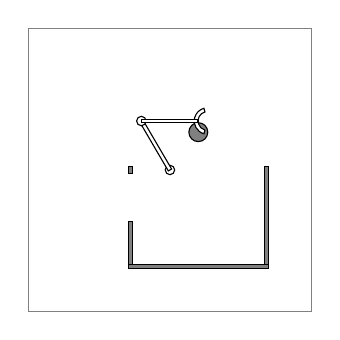
\begin{tikzpicture}
\begin{scope}[scale=1.2]
% bounding rect
\draw[color=black!50, thin] (-1.5,-1.5) rectangle (1.5,1.5);
\tikzstyle{dstyle}=[draw=black,fill=black!50]
\draw[dstyle] (0.300000,0.400000) circle (0.100000);
\draw[dstyle, shift={(0.300000,-1.020000)}, rotate=0.000000] (-0.740000,-0.020000) rectangle (0.740000,0.020000);
\draw[dstyle, shift={(1.020000,-0.480000)}, rotate=0.000000] (-0.020000,-0.520000) rectangle (0.020000,0.520000);
\draw[dstyle, shift={(-0.420000,-0.775000)}, rotate=0.000000] (-0.020000,-0.225000) rectangle (0.020000,0.225000);
\draw[dstyle, shift={(-0.420000,0.000000)}, rotate=0.000000] (-0.020000,-0.040000) rectangle (0.020000,0.040000);

\tikzstyle{dstyle}=[draw=black,fill=white]
\draw[dstyle] (0.000000,0.000000) circle (0.050000);
\draw[dstyle, shift={(-0.151454,0.258963)}, rotate=120.321137] (-0.300000,-0.020000) rectangle (0.300000,0.020000);
\draw[dstyle] (-0.302908,0.517926) circle (0.050000);
\draw[dstyle, shift={(0.397092,0.517926)}, rotate=180.000000](-74.484513:0.100000) arc (-74.484513:74.484513:0.100000) --(74.484513:0.140000) arc (74.484513:-74.484513:0.140000) -- cycle;
\draw[dstyle, shift={(-0.002908,0.517926)}, rotate=0.000000] (-0.300000,-0.020000) rectangle (0.300000,0.020000);

\end{scope}
\end{tikzpicture}
\caption{Invalid configuration}
\end{subfigure}%
\caption{Illustration of solution.}
\end{figure}

If we put some text in here, it shows up in the right place.

\begin{itemize}
\item comes from structure of multi-step problem
\item different cfrees
\item but they're very related!
\item inclusions, intersections
\end{itemize}

See Figure~\ref{fig:multi-set-example} for a simple motivating example.

\begin{figure}
\centering
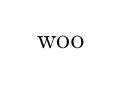
\begin{tikzpicture}

\node (a) at (0,0) {woo};

\end{tikzpicture}
\caption{An example of different $C_{free}$s}
\label{fig:multi-set-example}
\end{figure}

\subsection{Multiple sub-queries}

\subsection{Shared C-space}

\subsection{Each in a different C-free}

\subsection{Relations between C-frees (inclusion, intersection)}

\section{Related Work}

The topic of reusing planning computation
between similar motion planning problems
has been extensively studied in different domains.

\subsection{Explicit Configuration Spaces}

Early planning methods constructed explicit obstacles
directly in the configuration space.
This allows reuse via precomputed bitmaps
for translating robots \cite{kavraki1995cspacefft}
or via workspace primitives \cite{newmanbranicky1991cspacetransforms}.
One form of reuse is to precompute these for primitives.
More recently,
Lien and Lu \cite{lien2009similarobstacles} describe a method to
build a PRM around obstacles in a database,
and then reposes them in a new world.
The approach is not easily applicable to articulated robots
with complex mappings from workspace to C-space.

\subsection{Changing Free $\mathcal{C}$-Subsets}

Other approaches attempt to prune and grow graphs
within dynamically changing collision-free subsets,
e.g. the Dynamic RRT \cite{ferguson2006drrt},
the Reconfigurable Random Forest (RRF)
\cite{li2002incrementalprmmanagement},
and the Lazy Reconfiguration Forest
\cite{gayle2007lazyreconfigforest}.
%We do the lazy thing as well (built into our planner).
%None of these reason about the structure of the configuration space.
However, these approaches do not reason explicitly about the
structure of the configuration space.

\subsection{Static vs Dynamic Components of $\mathcal{C}_{free}$}

Some approaches do take advantage of such structure
through a two-level dichotomy between
permanent and non-permanent parts of $\mathcal{C}_{free}$.
Leven and Hutchinson \cite{leven2000changing}
and similar work \cite{kallman2004dynamicroadmaps}
handle changing environments by
precomputing a self-collision-free roadmap,
and then pruning it at query time
using a mapping from workspace cells to roadmap edges.
%This can also be viewed through the multi-space lens
%-- I think this is just an instantiation of a bunch of sets.
%They're very focused on the precomputation stuff.
%However, this approach this can't directly handle grasped objects.
Other methods \cite{jaillet2004dynamicprm}
exploit the dichotomy between static and dynamic parts of
the world online.

\subsection{Task and Motion Planning}

The structure in manipulation tasks that our approach leverages
is similar to the \emph{conditional reachability graph} which is
part of the recent \textsc{FFRob} heuristic task planning framework.
However, the framework is not incentivized to explore
areas of the configuration space that have already been explored.

\subsection{Fast Collision Checking}

Broad-phase collision checking.
See Section~\ref{subsec:broad-phase} for more on this.
I need cites!

\subsection{Sampling Strategies}

Also Kurniawati and Hsu's
\emph{Workspace-based Connectivity Oracle}
\cite{kurniawati2008workconnoracle}
which is a smart sampling strategy which considers workspace
geometry to inform PRM sampling.
Kurniawati has a bunch of other work on PRM fundamentals and sampling.
I think our approach is complementary to a PRM sampling strategy.
Or, you could do deterministic sampling
\cite{lavalle2002gridprms} \cite{geraerts2002prmcomparison}.

\subsection{Multi-Resolution Planning}

\noindent
\begin{itemize}
\item S. Kambhampati 1986
\item R. Steffens 2010
\item S. Zickler 2010
\item K. Gochev 2013
\end{itemize}

\subsection{Graph Search}

Many graph-search approaches are relevant to planning in similar
environments.
Algorithms such as
D* \cite{stentz1994dstar}
or LPA* \cite{koenig2004lpastar}
handle dynamically changing (or incrementally discovered) worlds.
Experience graphs \cite{phillips2012egraphs} are a method to apply
computation from previous graph-search planning queries
to the current problem.
The \textsc{BUGSY} algorithm \cite{ruml2007bugsy}
is most similar to our approach in the way that it explicitly
trades off between planning and execution (solution) cost.

\subsection{Other Related Work to Integrate}

Symbolic planning frameworks.

Newman and Branicky,
\emph{Real-Time Configuration Space Transforms for Obstacle Avoidance}
\cite{newmanbranicky1991cspacetransforms}
is a way to reuse stuff in related worlds.
From Sidd:
\begin{quote}
i know i've told you this before,
but it reminds me of how back in the day
people used to construct cobs
by stamping together cobs for primitives;
it's a form of reuse;
caching old cobs and transforming them for new problems

Here's a paper that talks about approximating C-obstacles.
They have a nice [obvious] theorem in 5.2. Set Containment Property.
\end{quote}

Also \cite{kavraki1995cspacefft}?

Also Kurniawati and Hsu's
\emph{Workspace-based Connectivity Oracle}
\cite{kurniawati2008workconnoracle}
which is a smart sampling strategy which considers workspace
geometry to inform PRM sampling.
Kurniawati has a bunch of other work on PRM fundamentals and sampling.

Jaillet and Simeon,
\emph{A PRM-based motion planner for dynamically changing environments}
\cite{jaillet2004dynamicprm}.
Explicit dichotomy between static and dynamic parts of the world.
Edges are checked when needed against moving obstacles;
their free-ness with respect to each is cached for the last tested position
for each obstacle.

Gayle, Klingler, and Xavier,
\emph{Lazy Reconfiguration Forest}
\cite{gayle2007lazyreconfigforest}.

Li and Shie,
\emph{An incremental learning approach to motion planning with
      roadmap management}
\cite{li2002incrementalprmmanagement}.
This is the Reconfigurable Random Forest (RRF).
They do ``roadmap management'' to handle changing environments,
and talk about doing some simple bounding-box stuff.

Lien and Lu,
\emph{Planning motion in environments with similar obstacles}
\cite{lien2009similarobstacles}.
This builds a PRM around obstacles in a database,
and then reposes them in a new world.

This is very similar to the \emph{conditional reachability graph}
presented by Garrett, Lozano-Perez, and Kaelbling
\cite{garrett2014ffrob}
as part of their task and motion symbolic planning mumbo-jumbo!

Also similar to the way changing environments are handled in PRMs
from Leven and Hutchinson \cite{leven2002changing}.

\section{Multi-Set Problem Formulation}
\label{sec:multi-set}

\begin{figure*}
\begin{widepage}
\centering

\begin{subfigure}[t]{.32\linewidth}
\centering
\documentclass{standalone}
\usepackage{tikz}
%\usetikzlibrary{...}
\begin{document}
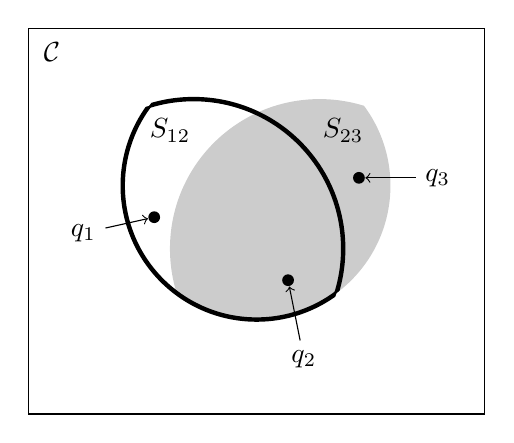
\begin{tikzpicture}

\draw (0,0) rectangle (5.8,4.9);

\coordinate (x) at (2.9,2.9);
\coordinate (y) at (2.1,2.1);
\coordinate (z) at (3.7,2.1);

\def\circlex{(x) circle (1.7)}
\def\circley{(y) circle (1.9)}
\def\circlez{(z) circle (1.9)}

% XnZ
\begin{scope}
   \clip \circlex;
   \fill[color=black!20] \circlez;
\end{scope}

% XnY
\begin{scope}
   \clip \circlex;
   %\fill[pattern=horizontal lines] \circley;
   \draw[ultra thick] \circley;
\end{scope}
\begin{scope}
   \clip \circley;
   \draw[ultra thick] \circlex;
\end{scope}

\node (clab) at (0.3,4.6) {$\mathcal{C}$};
\node[fill=white,circle,inner sep=0] (f1lab) at (1.8,3.6) {$S_{12}$};
\node (f2lab) at (4.0,3.6) {$S_{23}$};

\node[circle,fill=black,inner sep=1.5] (p1) at (1.6,2.5) {};
\node[circle,fill=black,inner sep=1.5] (p2) at (3.3,1.7) {};
\node[circle,fill=black,inner sep=1.5] (p3) at (4.2,3) {};

\node (p1lab) at (0.7,2.3) {$q_1$};
\node (p2lab) at (3.5,0.7) {$q_2$};
\node (p3lab) at (5.2,3.0) {$q_3$};
\draw[->] (p1lab) -- (p1);
\draw[->] (p2lab) -- (p2);
\draw[->] (p3lab) -- (p3);

\end{tikzpicture}%
\end{document}

\caption{A two-part multi-set problem in $\mathcal{C}$,
  first between $x_1$ and $x_2$ through $X_{12}$,
  then between $x_2$ and $x_3$ through $X_{23}$.
  The two free sets $X_{12}$ and $X_{23}$ are distinct
  but related.}
\end{subfigure}%
\quad%
\begin{subfigure}[t]{.32\linewidth}
\centering
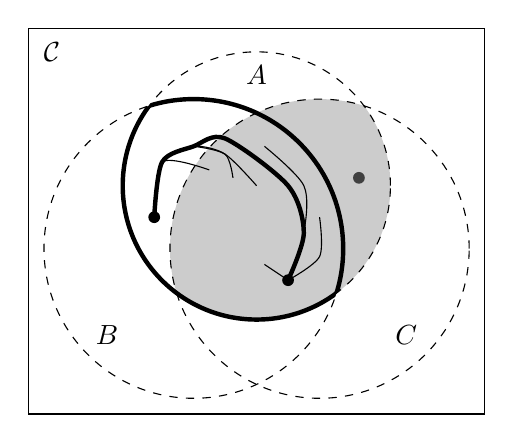
\begin{tikzpicture}

\draw (0,0) rectangle (5.8,4.9);

\coordinate (x) at (2.9,2.9);
\coordinate (y) at (2.1,2.1);
\coordinate (z) at (3.7,2.1);

\def\circlex{(x) circle (1.7)}
\def\circley{(y) circle (1.9)}
\def\circlez{(z) circle (1.9)}

% XnZ
\begin{scope}
   \clip \circlex;
   \fill[color=black!20] \circlez;
\end{scope}

% XnY
\begin{scope}
   \clip \circlex;
   %\fill[pattern=horizontal lines] \circley;
   \draw[ultra thick] \circley;
\end{scope}
\begin{scope}
   \clip \circley;
   \draw[ultra thick] \circlex;
\end{scope}

\draw[dashed] \circlex;
\draw[dashed] \circley;
\draw[dashed] \circlez;

\node (clab) at (0.3,4.6) {$\mathcal{C}$};
\node (xlab) at ($ (x) + (0,1.4) $) {$A$};
\node (ylab) at ($ (y) + (-1.1,-1.1) $) {$B$};
\node (zlab) at ($ (z) + ( 1.1,-1.1) $) {$C$};

\node[circle,fill=black,inner sep=1.5] (p1) at (1.6,2.5) {};
\node[circle,fill=black,inner sep=1.5] (p2) at (3.3,1.7) {};
\node[circle,fill=black!75,inner sep=1.5] (p3) at (4.2,3) {};

\draw plot [smooth] coordinates {
  (p1) (1.7,3.2) (2.3,3.1)};
\draw plot [smooth] coordinates {
  (p1) (1.7,3.2) (2.1,3.4) (2.5,3.3) (2.6,3.0)};
\draw plot [smooth] coordinates {
  (2.1,3.4) (2.5,3.3) (2.9,2.9)};
\draw plot [smooth] coordinates {
  (p2) (3.0,1.9)};
\draw plot [smooth] coordinates {
  (p2) (3.7,2.0) (3.7,2.5)};
\draw plot [smooth] coordinates {
  (p2) (3.5,2.3) (3.5,2.9) (3.0,3.4)};
\draw[ultra thick] plot [smooth] coordinates {
  (p1) (1.7,3.2) (2.1,3.4) (2.5,3.5) (3.3,2.9) (3.5,2.3) (p2)};

\end{tikzpicture}%

\caption{The free sets are related via other underlying
  subsets of $\mathcal{C}$, with $X_{12}=A \cap B$
  and $X_{23}=A \cap C$.
  A planner solving the first part (from $x_1$ to $x_2$)
  has found paths within $X_{12}$.}
\label{subfig:figstar-intersections}
\end{subfigure}%
\quad%
\begin{subfigure}[t]{.32\linewidth}
\centering
\documentclass{standalone}
\usepackage{tikz}
\usetikzlibrary{calc}
\begin{document}
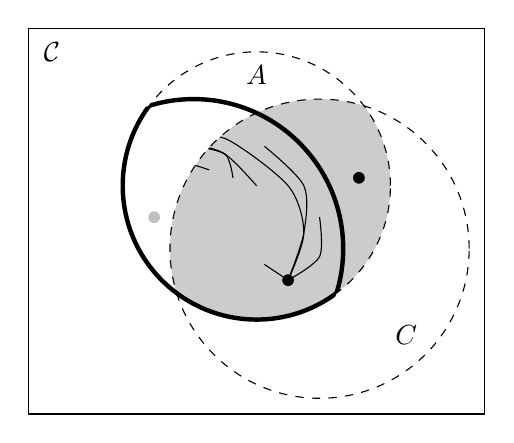
\begin{tikzpicture}

\draw (0,0) rectangle (5.8,4.9);

\coordinate (x) at (2.9,2.9);
\coordinate (y) at (2.1,2.1);
\coordinate (z) at (3.7,2.1);

\def\circlex{(x) circle (1.7)}
\def\circley{(y) circle (1.9)}
\def\circlez{(z) circle (1.9)}

% XnZ
\begin{scope}
   \clip \circlex;
   \fill[color=black!20] \circlez;
\end{scope}

% XnY
\begin{scope}
   \clip \circlex;
   %\fill[pattern=horizontal lines] \circley;
   \draw[ultra thick] \circley;
\end{scope}
\begin{scope}
   \clip \circley;
   \draw[ultra thick] \circlex;
\end{scope}

\draw[dashed] \circlex;
%\draw \circley;
\draw[dashed] \circlez;

\node (clab) at (0.3,4.6) {$\mathcal{C}$};
\node (xlab) at ($ (x) + (0,1.4) $) {$A$};
%\node (ylab) at ($ (y) + (-1.1,-1.1) $) {$B$};
\node (zlab) at ($ (z) + ( 1.1,-1.1) $) {$C$};

\node[circle,fill=black!25,inner sep=1.5] (p1) at (1.6,2.5) {};
\node[circle,fill=black,inner sep=1.5] (p2) at (3.3,1.7) {};
\node[circle,fill=black,inner sep=1.5] (p3) at (4.2,3) {};

\begin{scope}
  \clip \circlez;
  \draw plot [smooth] coordinates {
    (p1) (1.7,3.2) (2.3,3.1)};
  \draw plot [smooth] coordinates {
    (p1) (1.7,3.2) (2.1,3.4) (2.5,3.3) (2.6,3.0)};
  \draw plot [smooth] coordinates {
    (2.1,3.4) (2.5,3.3) (2.9,2.9)};
  \draw plot [smooth] coordinates {
    (p2) (3.0,1.9)};
  \draw plot [smooth] coordinates {
    (p2) (3.7,2.0) (3.7,2.5)};
  \draw plot [smooth] coordinates {
    (p2) (3.5,2.3) (3.5,2.9) (3.0,3.4)};
  \draw plot [smooth] coordinates {
    (p1) (1.7,3.2) (2.1,3.4) (2.5,3.5) (3.3,2.9) (3.5,2.3) (p2)};
\end{scope}

\end{tikzpicture}%
\end{document}

\caption{Due to the set relations,
  a planner solving the second part
  (from $x_2$ to $x_3$ in $X_{23}$)
  can reuse any segment known to be in $X_{12}$
  by checking only for its membership in $C$.}
\end{subfigure}

\vspace{0.1in}

\begin{subfigure}[t]{.32\linewidth}
\centering
\documentclass{standalone}
\usepackage{tikz}
%\usetikzlibrary{...}
\begin{document}
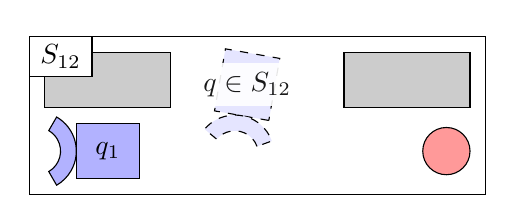
\begin{tikzpicture}

\draw (0,0) rectangle (5.8,2);

\draw[black,fill=black!20] (0.2,1.1) rectangle (1.8,1.8);
\draw[black,fill=black!20] (4.0,1.1) rectangle (5.6,1.8);

% robot (x1)
\begin{scope}[shift={(0.6,0.55)}]
   \draw[black,fill=blue!30] (0.0,-0.35) rectangle (0.8,0.35);
   \node at (0.4,0) {$q_1$};
   \draw[black,fill=blue!30,shift={(-0.5,0.0)}]
      (-60:0.3) arc (-60:60:0.3) -- (60:0.5) arc (60:-60:0.5) -- cycle;
   %\draw[black,fill=red!40] (-0.5,0) circle (0.3);
\end{scope}

% robot (x2)
\begin{scope}[shift={(4.8,0.55)},rotate=180]
   %\draw[black,fill=blue!30] (0.0,-0.35) rectangle (0.8,0.35);
   %\draw[black,fill=blue!30,shift={(-0.5,0.0)}]
   %   (-60:0.3) arc (-60:60:0.3) -- (60:0.5) arc (60:-60:0.5) -- cycle;
   \draw[black,fill=red!40] (-0.5,0) circle (0.3);
\end{scope}

% robot (x3)
%\begin{scope}[shift={(4.8,0.55)}]
%   \draw[black,fill=blue!30] (0.0,-0.35) rectangle (0.8,0.35);
%   \draw[black,fill=blue!30,shift={(-0.5,0.0)}]
%      (-60:0.3) arc (-60:60:0.3) -- (60:0.5) arc (60:-60:0.5) -- cycle;
%   \draw[black,fill=red!40] (-0.5,0) circle (0.3);
%\end{scope}

% robot (intermediate)
\begin{scope}[shift={(2.7,1.0)},rotate=80]
   \draw[black,fill=blue!10,dashed] (0.0,-0.35) rectangle (0.8,0.35);
   \draw[black,fill=blue!10,dashed,shift={(-0.5,0.0)}]
      (-60:0.3) arc (-60:60:0.3) -- (60:0.5) arc (60:-60:0.5) -- cycle;
   %\draw[black,fill=red!40] (-0.5,0) circle (0.3);
   \node[fill=white,fill opacity=0.9] at (0.4,0) {$q \in S_{12}$};
\end{scope}

% label
\draw[fill=white] (0,1.5) rectangle (0.8,2);
\node at (0.4,1.75) {$S_{12}$};

% for vertical spacing
\node[inner sep=0] at (0,2.1) {};

\end{tikzpicture}%
\end{document}

\documentclass{standalone}
\usepackage{tikz}
%\usetikzlibrary{...}
\begin{document}
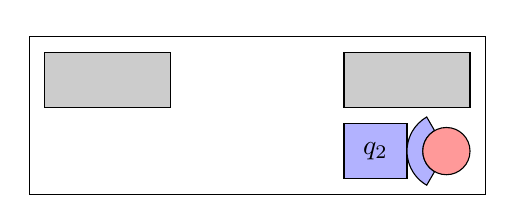
\begin{tikzpicture}

\draw (0,0) rectangle (5.8,2);

\draw[black,fill=black!20] (0.2,1.1) rectangle (1.8,1.8);
\draw[black,fill=black!20] (4.0,1.1) rectangle (5.6,1.8);

% robot (x1)
%\begin{scope}[shift={(0.6,0.55)}]
%   \draw[black,fill=blue!30] (0.0,-0.35) rectangle (0.8,0.35);
%   \node at (0.4,0) {$x_1$};
%   \draw[black,fill=blue!30,shift={(-0.5,0.0)}]
%      (-60:0.3) arc (-60:60:0.3) -- (60:0.5) arc (60:-60:0.5) -- cycle;
%   \draw[black,fill=red!40] (-0.5,0) circle (0.3);
%\end{scope}

% robot (x2)
\begin{scope}[shift={(4.8,0.55)},rotate=180]
   \draw[black,fill=blue!30] (0.0,-0.35) rectangle (0.8,0.35);
   \node at (0.4,0) {$q_2$};
   \draw[black,fill=blue!30,shift={(-0.5,0.0)}]
      (-60:0.3) arc (-60:60:0.3) -- (60:0.5) arc (60:-60:0.5) -- cycle;
   \draw[black,fill=red!40] (-0.5,0) circle (0.3);
\end{scope}

% robot (x3)
%\begin{scope}[shift={(4.8,0.55)}]
%   \draw[black,fill=blue!30] (0.0,-0.35) rectangle (0.8,0.35);
%   \draw[black,fill=blue!30,shift={(-0.5,0.0)}]
%      (-60:0.3) arc (-60:60:0.3) -- (60:0.5) arc (60:-60:0.5) -- cycle;
%   \draw[black,fill=red!40] (-0.5,0) circle (0.3);
%\end{scope}

% robot (intermediate)
%\begin{scope}[shift={(2.7,1.0)},rotate=80]
%   \draw[black,dashed] (0.0,-0.35) rectangle (0.8,0.35);
%   \draw[black,dashed,shift={(-0.5,0.0)}]
%      (-60:0.3) arc (-60:60:0.3) -- (60:0.5) arc (60:-60:0.5) -- cycle;
%   %\draw[black,fill=red!40] (-0.5,0) circle (0.3);
%\end{scope}

% label
%\draw[fill=white] (0,1.5) rectangle (0.8,2);
%\node at (0.4,1.75) {$X_{12}$};

% for vertical spacing
\node[inner sep=0] at (0,2.1) {};

\end{tikzpicture}%
\end{document}

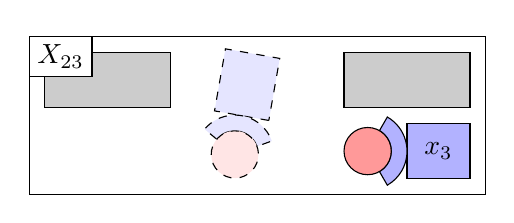
\begin{tikzpicture}

\draw (0,0) rectangle (5.8,2);

\draw[black,fill=black!20] (0.2,1.1) rectangle (1.8,1.8);
\draw[black,fill=black!20] (4.0,1.1) rectangle (5.6,1.8);

% robot (x1)
%\begin{scope}[shift={(0.6,0.55)}]
%   \draw[black,fill=blue!30] (0.0,-0.35) rectangle (0.8,0.35);
%   \node at (0.4,0) {$x_1$};
%   \draw[black,fill=blue!30,shift={(-0.5,0.0)}]
%      (-60:0.3) arc (-60:60:0.3) -- (60:0.5) arc (60:-60:0.5) -- cycle;
%   %\draw[black,fill=red!40] (-0.5,0) circle (0.3);
%\end{scope}

% robot (x2)
%\begin{scope}[shift={(4.8,0.55)},rotate=180]
%   %\draw[black,fill=blue!30] (0.0,-0.35) rectangle (0.8,0.35);
%   %\draw[black,fill=blue!30,shift={(-0.5,0.0)}]
%   %   (-60:0.3) arc (-60:60:0.3) -- (60:0.5) arc (60:-60:0.5) -- cycle;
%   \draw[black,fill=red!40] (-0.5,0) circle (0.3);
%\end{scope}

% robot (x3)
\begin{scope}[shift={(4.8,0.55)}]
   \draw[black,fill=blue!30] (0.0,-0.35) rectangle (0.8,0.35);
   \node at (0.4,0) {$x_3$};
   \draw[black,fill=blue!30,shift={(-0.5,0.0)}]
      (-60:0.3) arc (-60:60:0.3) -- (60:0.5) arc (60:-60:0.5) -- cycle;
   \draw[black,fill=red!40] (-0.5,0) circle (0.3);
\end{scope}

% robot (intermediate)
\begin{scope}[shift={(2.7,1.0)},rotate=80]
   \draw[black,fill=blue!10,dashed] (0.0,-0.35) rectangle (0.8,0.35);
   \draw[black,fill=blue!10,dashed,shift={(-0.5,0.0)}]
      (-60:0.3) arc (-60:60:0.3) -- (60:0.5) arc (60:-60:0.5) -- cycle;
   \draw[black,fill=red!10,dashed] (-0.5,0) circle (0.3);
\end{scope}

% label
\draw[fill=white] (0,1.5) rectangle (0.8,2);
\node at (0.4,1.75) {$X_{23}$};

% for vertical spacing
\node[inner sep=0] at (0,2.1) {};

\end{tikzpicture}%

\caption{A forklift in a parking lot ($x_1$)
  must retrieve an object ($x_2$)
  and reverse park ($x_3$).
  This two-part problem
  requires plans in distinct collision-free
  $\mathcal{C}$-subsets
  $X_{12}$ and $X_{23}$.}
\label{subfig:figstar-manip-probdef}
\end{subfigure}%
\quad%
\begin{subfigure}[t]{.32\linewidth}
\centering
\documentclass{standalone}
\usepackage{tikz}
%\usetikzlibrary{...}
\begin{document}
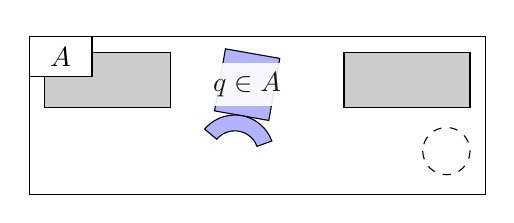
\begin{tikzpicture}

\draw (0,0) rectangle (5.8,2);

\draw[black,fill=black!20] (0.2,1.1) rectangle (1.8,1.8);
\draw[black,fill=black!20] (4.0,1.1) rectangle (5.6,1.8);

% robot (x1)
%\begin{scope}[shift={(0.6,0.55)}]
%   \draw[black,fill=blue!30] (0.0,-0.35) rectangle (0.8,0.35);
%   \node at (0.4,0) {$x_1$};
%   \draw[black,fill=blue!30,shift={(-0.5,0.0)}]
%      (-60:0.3) arc (-60:60:0.3) -- (60:0.5) arc (60:-60:0.5) -- cycle;
%   %\draw[black,fill=red!40] (-0.5,0) circle (0.3);
%\end{scope}

% robot (x2)
\begin{scope}[shift={(4.8,0.55)},rotate=180]
   %\draw[black,fill=blue!30] (0.0,-0.35) rectangle (0.8,0.35);
   %\draw[black,fill=blue!30,shift={(-0.5,0.0)}]
   %   (-60:0.3) arc (-60:60:0.3) -- (60:0.5) arc (60:-60:0.5) -- cycle;
   \draw[black,dashed] (-0.5,0) circle (0.3);
\end{scope}

% robot (x3)
%\begin{scope}[shift={(4.8,0.55)}]
%   \draw[black,fill=blue!30] (0.0,-0.35) rectangle (0.8,0.35);
%   \draw[black,fill=blue!30,shift={(-0.5,0.0)}]
%      (-60:0.3) arc (-60:60:0.3) -- (60:0.5) arc (60:-60:0.5) -- cycle;
%   \draw[black,fill=red!40] (-0.5,0) circle (0.3);
%\end{scope}

% robot (intermediate)
\begin{scope}[shift={(2.7,1.0)},rotate=80]
   \draw[black,fill=blue!30] (0.0,-0.35) rectangle (0.8,0.35);
   \draw[black,fill=blue!30,shift={(-0.5,0.0)}]
      (-60:0.3) arc (-60:60:0.3) -- (60:0.5) arc (60:-60:0.5) -- cycle;
   %\draw[black,fill=red!40] (-0.5,0) circle (0.3);
   \node[fill=white,fill opacity=0.9] at (0.4,0) {$q \in A$};
\end{scope}

% label
\draw[fill=white] (0,1.5) rectangle (0.8,2);
\node at (0.4,1.75) {$A$};

% for vertical spacing
\node[inner sep=0] at (0,2.1) {};

\end{tikzpicture}%
\end{document}

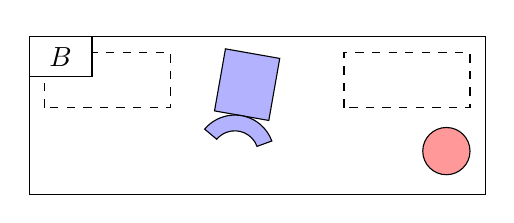
\begin{tikzpicture}

\draw (0,0) rectangle (5.8,2);

\draw[black,dashed] (0.2,1.1) rectangle (1.8,1.8);
\draw[black,dashed] (4.0,1.1) rectangle (5.6,1.8);

% robot (x1)
%\begin{scope}[shift={(0.6,0.55)}]
%   \draw[black,fill=blue!30] (0.0,-0.35) rectangle (0.8,0.35);
%   \node at (0.4,0) {$x_1$};
%   \draw[black,fill=blue!30,shift={(-0.5,0.0)}]
%      (-60:0.3) arc (-60:60:0.3) -- (60:0.5) arc (60:-60:0.5) -- cycle;
%   %\draw[black,fill=red!40] (-0.5,0) circle (0.3);
%\end{scope}

% robot (x2)
\begin{scope}[shift={(4.8,0.55)},rotate=180]
   %\draw[black,fill=blue!30] (0.0,-0.35) rectangle (0.8,0.35);
   %\draw[black,fill=blue!30,shift={(-0.5,0.0)}]
   %   (-60:0.3) arc (-60:60:0.3) -- (60:0.5) arc (60:-60:0.5) -- cycle;
   \draw[black,fill=red!40] (-0.5,0) circle (0.3);
\end{scope}

% robot (x3)
%\begin{scope}[shift={(4.8,0.55)}]
%   \draw[black,fill=blue!30] (0.0,-0.35) rectangle (0.8,0.35);
%   \draw[black,fill=blue!30,shift={(-0.5,0.0)}]
%      (-60:0.3) arc (-60:60:0.3) -- (60:0.5) arc (60:-60:0.5) -- cycle;
%   \draw[black,fill=red!40] (-0.5,0) circle (0.3);
%\end{scope}

% robot (intermediate)
\begin{scope}[shift={(2.7,1.0)},rotate=80]
   \draw[black,fill=blue!30] (0.0,-0.35) rectangle (0.8,0.35);
   \draw[black,fill=blue!30,shift={(-0.5,0.0)}]
      (-60:0.3) arc (-60:60:0.3) -- (60:0.5) arc (60:-60:0.5) -- cycle;
   %\draw[black,fill=red!40] (-0.5,0) circle (0.3);
\end{scope}

% label
\draw[fill=white] (0,1.5) rectangle (0.8,2);
\node at (0.4,1.75) {$B$};

% for vertical spacing
\node[inner sep=0] at (0,2.1) {};

\end{tikzpicture}%

\documentclass{standalone}
\usepackage{tikz}
%\usetikzlibrary{...}
\begin{document}
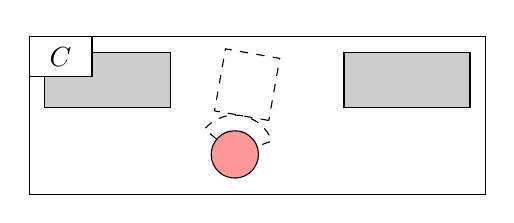
\begin{tikzpicture}

\draw (0,0) rectangle (5.8,2);

\draw[black,fill=black!20] (0.2,1.1) rectangle (1.8,1.8);
\draw[black,fill=black!20] (4.0,1.1) rectangle (5.6,1.8);

% robot (x1)
%\begin{scope}[shift={(0.6,0.55)}]
%   \draw[black,fill=blue!30] (0.0,-0.35) rectangle (0.8,0.35);
%   \node at (0.4,0) {$x_1$};
%   \draw[black,fill=blue!30,shift={(-0.5,0.0)}]
%      (-60:0.3) arc (-60:60:0.3) -- (60:0.5) arc (60:-60:0.5) -- cycle;
%   %\draw[black,fill=red!40] (-0.5,0) circle (0.3);
%\end{scope}

% robot (x2)
%\begin{scope}[shift={(4.8,0.55)},rotate=180]
%   %\draw[black,fill=blue!30] (0.0,-0.35) rectangle (0.8,0.35);
%   %\draw[black,fill=blue!30,shift={(-0.5,0.0)}]
%   %   (-60:0.3) arc (-60:60:0.3) -- (60:0.5) arc (60:-60:0.5) -- cycle;
%   \draw[black,fill=red!40] (-0.5,0) circle (0.3);
%\end{scope}

% robot (x3)
%\begin{scope}[shift={(4.8,0.55)}]
%   \draw[black,fill=blue!30] (0.0,-0.35) rectangle (0.8,0.35);
%   \draw[black,fill=blue!30,shift={(-0.5,0.0)}]
%      (-60:0.3) arc (-60:60:0.3) -- (60:0.5) arc (60:-60:0.5) -- cycle;
%   \draw[black,fill=red!40] (-0.5,0) circle (0.3);
%\end{scope}

% robot (intermediate)
\begin{scope}[shift={(2.7,1.0)},rotate=80]
   \draw[black,dashed] (0.0,-0.35) rectangle (0.8,0.35);
   \draw[black,dashed,shift={(-0.5,0.0)}]
      (-60:0.3) arc (-60:60:0.3) -- (60:0.5) arc (60:-60:0.5) -- cycle;
   \draw[black,fill=red!40] (-0.5,0) circle (0.3);
\end{scope}

% label
\draw[fill=white] (0,1.5) rectangle (0.8,2);
\node at (0.4,1.75) {$C$};

% for vertical spacing
\node[inner sep=0] at (0,2.1) {};

\end{tikzpicture}%
\end{document}

\caption{Sets $X_{12}$ and $X_{23}$ are subsets of
  the configuration space of the robot $\mathcal{C}=\mbox{SE}(2)$,
  and can be represented as intersections
  of underlying subsets $A$, $B$, and $C$
  as in Fig.~\ref{subfig:figstar-intersections}.}
\label{subfig:figstar-manip-spaces}
\end{subfigure}%
\quad%
\begin{subfigure}[t]{.32\linewidth}
\centering
\documentclass{standalone}
\usepackage{tikz}
%\usetikzlibrary{...}
\begin{document}
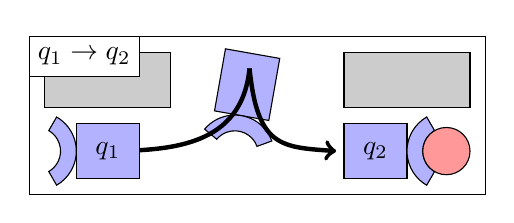
\begin{tikzpicture}

\draw (0,0) rectangle (5.8,2);

\draw[black,fill=black!20] (0.2,1.1) rectangle (1.8,1.8);
\draw[black,fill=black!20] (4.0,1.1) rectangle (5.6,1.8);

% robot (intermediate)
\begin{scope}[shift={(2.7,1.0)},rotate=80]
   \draw[black,fill=blue!30] (0.0,-0.35) rectangle (0.8,0.35);
   %\node at (0.4,0) {$x_i$};
   \draw[black,fill=blue!30,shift={(-0.5,0.0)}]
      (-60:0.3) arc (-60:60:0.3) -- (60:0.5) arc (60:-60:0.5) -- cycle;
   %\draw[black,fill=red!40] (-0.5,0) circle (0.3);
\end{scope}

\draw[ultra thick,black]
   (0.9,0.55) .. controls (1.8,0.55) and (2.7,0.6) .. (2.8,1.6);
\draw[ultra thick,black,->]
   (2.8,1.6) .. controls (2.9,0.6) and (3.2,0.6) .. (3.9,0.55);
%\node[circle,fill=black,inner sep=2] at (2.76,1.4) {};

% robot (x1)
\begin{scope}[shift={(0.6,0.55)}]
   \draw[black,fill=blue!30] (0.0,-0.35) rectangle (0.8,0.35);
   \node at (0.4,0) {$q_1$};
   \draw[black,fill=blue!30,shift={(-0.5,0.0)}]
      (-60:0.3) arc (-60:60:0.3) -- (60:0.5) arc (60:-60:0.5) -- cycle;
   %\draw[black,fill=red!40] (-0.5,0) circle (0.3);
\end{scope}

% robot (x2)
\begin{scope}[shift={(4.8,0.55)},rotate=180]
   \draw[black,fill=blue!30] (0.0,-0.35) rectangle (0.8,0.35);
   \node at (0.4,0) {$q_2$};
   \draw[black,fill=blue!30,shift={(-0.5,0.0)}]
      (-60:0.3) arc (-60:60:0.3) -- (60:0.5) arc (60:-60:0.5) -- cycle;
   \draw[black,fill=red!40] (-0.5,0) circle (0.3);
\end{scope}

% robot (x3)
%\begin{scope}[shift={(4.8,0.55)}]
%   \draw[black,fill=black!20] (0.0,-0.35) rectangle (0.8,0.35);
%   \draw[black,fill=black!20,shift={(-0.5,0.0)}]
%      (-60:0.3) arc (-60:60:0.3) -- (60:0.5) arc (60:-60:0.5) -- cycle;
%   \draw[black,fill=black!20] (-0.5,0) circle (0.3);
%\end{scope}

% label
\draw[fill=white] (0,1.5) rectangle (1.4,2);
\node at (0.7,1.75) {$q_1 \rightarrow q_2$};

%\draw plot [smooth] coordinates {
%  (0.9,0.55) (1.8,0.6) (2.4,0.9) (2.6,1.2) (2.7,1.4)};


% for vertical spacing
\node[inner sep=0] at (0,2.1) {};

\end{tikzpicture}%
\end{document}

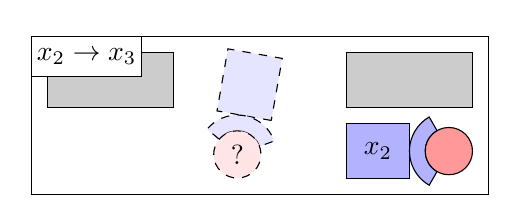
\begin{tikzpicture}

\draw (0,0) rectangle (5.8,2);

\draw[black,fill=black!20] (0.2,1.1) rectangle (1.8,1.8);
\draw[black,fill=black!20] (4.0,1.1) rectangle (5.6,1.8);

% robot (x1)
%\begin{scope}[shift={(0.6,0.55)}]
%   \draw[black,fill=blue!30] (0.0,-0.35) rectangle (0.8,0.35);
%   \node at (0.4,0) {$x_1$};
%   \draw[black,fill=blue!30,shift={(-0.5,0.0)}]
%      (-60:0.3) arc (-60:60:0.3) -- (60:0.5) arc (60:-60:0.5) -- cycle;
%   %\draw[black,fill=red!40] (-0.5,0) circle (0.3);
%\end{scope}

% robot (x2)
\begin{scope}[shift={(4.8,0.55)},rotate=180]
   \draw[black,fill=blue!30] (0.0,-0.35) rectangle (0.8,0.35);
   \node at (0.4,0) {$x_2$};
   \draw[black,fill=blue!30,shift={(-0.5,0.0)}]
      (-60:0.3) arc (-60:60:0.3) -- (60:0.5) arc (60:-60:0.5) -- cycle;
   \draw[black,fill=red!40] (-0.5,0) circle (0.3);
\end{scope}

% robot (x3)
%\begin{scope}[shift={(4.8,0.55)}]
%   \draw[black,fill=blue!30] (0.0,-0.35) rectangle (0.8,0.35);
%   \draw[black,fill=blue!30,shift={(-0.5,0.0)}]
%      (-60:0.3) arc (-60:60:0.3) -- (60:0.5) arc (60:-60:0.5) -- cycle;
%   \draw[black,fill=red!40] (-0.5,0) circle (0.3);
%\end{scope}

% robot (intermediate)
\begin{scope}[shift={(2.7,1.0)},rotate=80]
   \draw[black,fill=blue!10,dashed] (0.0,-0.35) rectangle (0.8,0.35);
   \draw[black,fill=blue!10,dashed,shift={(-0.5,0.0)}]
      (-60:0.3) arc (-60:60:0.3) -- (60:0.5) arc (60:-60:0.5) -- cycle;
   \draw[black,fill=red!10,dashed] (-0.5,0) circle (0.3);
   \node at (-.5,0) {?};
\end{scope}

% label
\draw[fill=white] (0,1.5) rectangle (1.4,2);
\node at (0.7,1.75) {$x_2 \rightarrow x_3$};

% for vertical spacing
\node[inner sep=0] at (0,2.1) {};

\end{tikzpicture}%

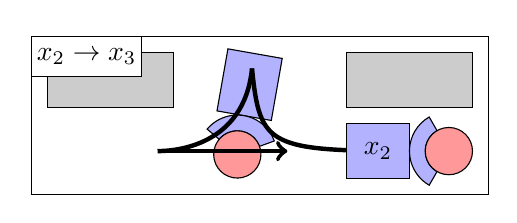
\begin{tikzpicture}

\draw (0,0) rectangle (5.8,2);

\draw[black,fill=black!20] (0.2,1.1) rectangle (1.8,1.8);
\draw[black,fill=black!20] (4.0,1.1) rectangle (5.6,1.8);

% robot (intermediate)
\begin{scope}[shift={(2.7,1.0)},rotate=80]
   \draw[black,fill=blue!30] (0.0,-0.35) rectangle (0.8,0.35);
   \draw[black,fill=blue!30,shift={(-0.5,0.0)}]
      (-60:0.3) arc (-60:60:0.3) -- (60:0.5) arc (60:-60:0.5) -- cycle;
   \draw[black,fill=red!40] (-0.5,0) circle (0.3);
\end{scope}

\draw[ultra thick,black]
   (1.6,0.55) .. controls (1.8,0.55) and (2.7,0.6) .. (2.8,1.6);
\draw[ultra thick,black]
   (2.8,1.6) .. controls (2.9,0.6) and (3.0,0.55) .. (4.9,0.55);
\draw[ultra thick,black,->]
   (1.6,0.55) -- (3.25,0.55);
%\node[circle,fill=black,inner sep=2] at (2.76,1.4) {};

% robot (x1)
%\begin{scope}[shift={(0.6,0.55)}]
%   \draw[black,fill=blue!30] (0.0,-0.35) rectangle (0.8,0.35);
%   \node at (0.4,0) {$x_1$};
%   \draw[black,fill=blue!30,shift={(-0.5,0.0)}]
%      (-60:0.3) arc (-60:60:0.3) -- (60:0.5) arc (60:-60:0.5) -- cycle;
%   %\draw[black,fill=red!40] (-0.5,0) circle (0.3);
%\end{scope}

% robot (x2)
\begin{scope}[shift={(4.8,0.55)},rotate=180]
   \draw[black,fill=blue!30] (0.0,-0.35) rectangle (0.8,0.35);
   \node at (0.4,0) {$x_2$};
   \draw[black,fill=blue!30,shift={(-0.5,0.0)}]
      (-60:0.3) arc (-60:60:0.3) -- (60:0.5) arc (60:-60:0.5) -- cycle;
   \draw[black,fill=red!40] (-0.5,0) circle (0.3);
\end{scope}

% robot (x3)
%\begin{scope}[shift={(4.8,0.55)}]
%   \draw[black,fill=blue!30] (0.0,-0.35) rectangle (0.8,0.35);
%   \node at (0.4,0) {$x_3$};
%   \draw[black,fill=blue!30,shift={(-0.5,0.0)}]
%      (-60:0.3) arc (-60:60:0.3) -- (60:0.5) arc (60:-60:0.5) -- cycle;
%   \draw[black,fill=red!40] (-0.5,0) circle (0.3);
%\end{scope}

% label
\draw[fill=white] (0,1.5) rectangle (1.4,2);
\node at (0.7,1.75) {$x_2 \rightarrow x_3$};

% for vertical spacing
\node[inner sep=0] at (0,2.1) {};

\end{tikzpicture}%

\caption{After planning a path from $x_1$ to $x_2$ (top),
  a planner can reuse a configuration in $X_{12}$ (middle)
  by checking only for its membership in subset $C$,
  resulting in plan reuse (bottom).}
\end{subfigure}

\caption{An illustration of a multi-set planning
  problem in a common configuration space $\mathcal{C}$.
  The problem definition generalizes to an artibrary number of
  configuration space subsets and set relations between them.
  When two queries in different subests are solved sequentially,
  a multi-set planner can reuse path segments less expensively.
  See Section~\ref{sec:in-manipulation} for examples in
  manipulation.}
\label{fig:multi-set}
\end{widepage}
\end{figure*}

Here we define the multi-set planning problem,
a generalization of both the movers' problem
and the multi-query planning problem
\cite{kavrakietal1996prm}.
The reader is referred to
Fig.~\ref{fig:multi-set}
for a general example,
as well as a simple instantiation in a 2D manipulation task.
%which is discussed in more detail in
%Section~\ref{subsec:multi-prm-example}.
The multi-set problem formulation
explicitly captures both planning and
solution (execution) cost.

\subsection{Formal Multi-Set Problem Definition}
\label{subsec:problem-definition}

The multi-set planning problem is multi-query in
a fixed configuration space $\mathcal{C}$.
However, unlike related problems in which all
queries demand solution paths contained within a single common subset of
$\mathcal{C}$
(usually the set of collision-free configurations, denoted
$\mathcal{C}_{free}$),
the multi-set problem allows for the specification of
\emph{multiple} such $\mathcal{C}$-subsets
$\mathcal{S} = \{ A, B, \dots \}$.
Like $\mathcal{C}_{free}$,
each member of $\mathcal{S}$
is a subset of the common configuration space
(that is,
$X \subseteq \mathcal{C} \;\forall\; X \in \mathcal{S}$).
For example, in Fig.~\ref{subfig:figstar-manip-spaces},
$\mathcal{C}$-subset $B$
consists of configurations
free of collision between the robot and
the initial object pose.

\begin{figure}
\centering
\begin{subfigure}[t]{0.45\linewidth}
\centering
\documentclass{standalone}
\usepackage{tikz}
%\usetikzlibrary{...}
\begin{document}
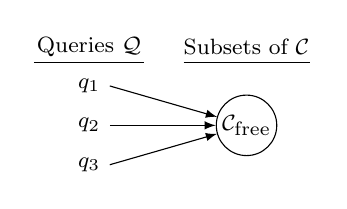
\begin{tikzpicture}
\tikzstyle{every node}=[font=\footnotesize]
\tikzset{>=latex} % arrow heads
\node at (1.0,-0.2) {Queries $\mathcal{Q}$};
\node at (3.0,-0.2) {Subsets of $\mathcal{C}$};
\draw (0.3,-0.4) -- (1.7,-0.4);
\draw (2.2,-0.4) -- (3.8,-0.4);
\node (q1) at (1.0,-0.7) {$q_1$};
\node (q2) at (1.0,-1.2) {$q_2$};
\node (q3) at (1.0,-1.7) {$q_3$};
\node[draw,circle,inner sep=1] (cfree) at (3.0,-1.2)
  {$\mathcal{C}_{\mbox{\scriptsize free}}$};
\draw[->] (q1.east) -- (cfree);
\draw[->] (q2.east) -- (cfree);
\draw[->] (q3.east) -- (cfree);
%\draw[step=1,black!10,very thin] (0,-2) grid (4,0);
\end{tikzpicture}%
\end{document}

\caption{Multi-query planning}
\end{subfigure}%
\quad\quad%
\begin{subfigure}[t]{0.45\linewidth}
\centering
\documentclass{standalone}
\usepackage{tikz}
%\usetikzlibrary{...}
\begin{document}
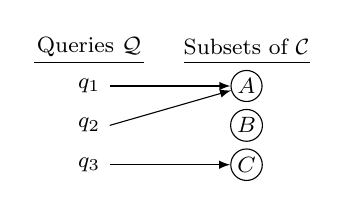
\begin{tikzpicture}
\tikzstyle{every node}=[font=\footnotesize]
\tikzset{>=latex} % arrow heads
\node at (1.0,-0.2) {Queries $\mathcal{Q}$};
\node at (3.0,-0.2) {Subsets of $\mathcal{C}$};
\draw (0.3,-0.4) -- (1.7,-0.4);
\draw (2.2,-0.4) -- (3.8,-0.4);
\node (q1) at (1.0,-0.7) {$q_1$};
\node (q2) at (1.0,-1.2) {$q_2$};
\node (q3) at (1.0,-1.7) {$q_3$};
\node[draw,circle,inner sep=1] (a) at (3.0,-0.7) {$A$};
\node[draw,circle,inner sep=1] (b) at (3.0,-1.2) {$B$};
\node[draw,circle,inner sep=1] (c) at (3.0,-1.7) {$C$};
\draw[->] (q1.east) -- (a);
\draw[->] (q2.east) -- (a);
\draw[->] (q3.east) -- (c);
%\draw[step=1,black!10,very thin] (0,-2) grid (4,0);
\end{tikzpicture}%
\end{document}

\caption{Multi-set planning}
\end{subfigure}
\caption{While queries in multi-query planning reference
  the same subset of $\mathcal{C}$,
  each multi-set query references one of a number of such sets.}
\label{fig:query-to-subset}
\end{figure}

The problem supports an arbitrary number of queries $\mathcal{Q}$.
Each query $q$ references a \emph{single}
$\mathcal{C}$-subset $X_q \in \mathcal{S}$
(see Fig~\ref{fig:query-to-subset}):
\begin{equation}
  q : ( x_{start},\; x_{goal},\; X_q ) .
  \label{eqn:q}
\end{equation}
A continuous feasible solution path $x(t)$ must then satisfy
\begin{equation}
  \begin{array}{c}
  x(t) \in X_q \;\forall\; t \in [0,1] \\
  x(0) = x_{start},\; x(1) = x_{goal} . \\
  \end{array}
  \label{eqn:solution}
\end{equation}
Eqns. (\ref{eqn:q}), (\ref{eqn:solution})
specify single configurations
$x_{start}$ and $x_{goal}$,
but the formulation is trivially extended to start/goal sets.

While simple problems may admit explicit representations of
subsets of $\mathcal{C}$,
recent approaches to complex problems
(e.g. sampling-based planners)
instead reason implicitly via test function(s)
\cite{lavalle2006planningbook}.
To capture this,
we endow each $\mathcal{C}$-subset $X \in \mathcal{S}$ with an
\emph{indicator function} $\mathbf{1}_X(x)$:
\begin{equation}
  \mathbf{1}_X(x) =
    \left\{ \begin{array}{ll}
      \mbox{True} & \mbox{if } x \in X \\
      \mbox{False} & \mbox{otherwise}.
    \end{array} \right.
  \label{eqn:indicator-function}
\end{equation}
Equivalently, the set itself can be defined w.r.t. its indicator:
\begin{equation}
  X = \{ x \in \mathcal{C} \;|\; \mathbf{1}_X(x) = \mbox{True} \} .
\end{equation}
Excusing the abuse of notation,
we define an analogous indicator functional $\mathbf{1}_X[\cdot]$
which operates on path segments $x(t)$.
We use parentheses for functions and brackets for functionals.
\begin{equation}
  \mathbf{1}_X[x(t)] =
    \left\{ \begin{array}{ll}
      \mbox{True} & \mbox{if } x(t) \in X \;\forall\; t \in [0,1] \\
      \mbox{False} & \mbox{otherwise}.
    \end{array} \right.
  \label{eqn:indicator-functional}
\end{equation}
Common examples of such indicators
(\ref{eqn:indicator-function}) or (\ref{eqn:indicator-functional})
include validity checkers for
geometric (workspace) collision,
stability, and visibility constraints.
Note that for complex problems,
evaluation of these indicators 
tends to dominate planning cost.

\begin{figure}
\centering
\begin{subfigure}[t]{0.45\linewidth}
\centering
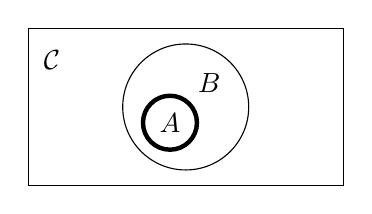
\begin{tikzpicture}
\draw (0,-2) rectangle (4,0);
\node (clab) at (0.3,-0.4) {$\mathcal{C}$};
\draw (2.0,-1.0) circle (0.8);
\node[draw,circle,ultra thick] at (1.8,-1.2) {$A$};
\node at (2.3,-0.7) {$B$};
\end{tikzpicture}%
 \\
$A \subseteq B$ \\
$\mathbf{1}_A \Rightarrow \mathbf{1}_B$
\caption{Containment relation}
\end{subfigure}%
\quad\quad%
\begin{subfigure}[t]{0.45\linewidth}
\centering
\documentclass{standalone}
\usepackage{tikz}
%\usetikzlibrary{...}
\begin{document}
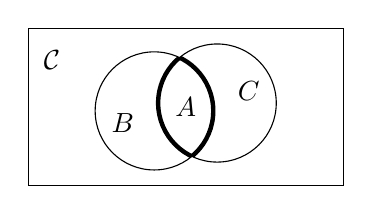
\begin{tikzpicture}
\draw (0,-2) rectangle (4,0);
\node (clab) at (0.3,-0.4) {$\mathcal{C}$};
\def\circleb{(1.6,-1.05) circle (0.75)}
\def\circlec{(2.4,-0.95) circle (0.75)}
\draw \circleb;
\draw \circlec;
\begin{scope}
   \clip \circleb;
   \draw[ultra thick] \circlec;
\end{scope}
\begin{scope}
   \clip \circlec;
   \draw[ultra thick] \circleb;
\end{scope}
\node at (2.0,-1.0) {$A$};
\node at (1.2,-1.2) {$B$};
\node at (2.8,-0.8) {$C$};
\end{tikzpicture}%
\end{document}
 \\
$A = B \cap C$ \\
$\mathbf{1}_B \wedge \mathbf{1}_C \Rightarrow \mathbf{1}_A$
\caption{Intersection relation}
\end{subfigure}
\caption{Types of relations used in the paper.
  Each relation can be expressed directly as set relations
  or equivalently as logical statements
  on the corresponding indicator functions
  $\mathbf{1}_X(\cdot)$.}
\label{fig:relations}
\end{figure}

Finally, the multi-set problem incudes a list of set relations
$\mathcal{R}$
between the $\mathcal{C}$-subsets in $\mathcal{S}$.
These can be expressed directly using set theoretic relations,
or equivalently as logical statements
on the corresponding indicator functions.
The two types of relations we use in this paper
(containment and intersection)
are described in Fig.~\ref{fig:relations}.
Fig.~\ref{fig:multi-set} gives an example of intersection relations;
an example of containment is a padded (conservative)
robot model (see Section~\ref{subsec:broad-phase}).

Together, these four elements
(a configuration space $\mathcal{C}$,
subsets $\mathcal{S}$ each with endowed indicators,
a set of queries $\mathcal{Q}$,
and a list of subset relations $\mathcal{R}$)
comprise a multi-set planning problem.

\subsection{Cost Model}
\label{subsec:cost-model}

While the indicators
(\ref{eqn:indicator-function}) and (\ref{eqn:indicator-functional})
are binary,
we are often interested not only in solution feasibility,
but also minimizing a measure of \emph{execution cost}
on the solution path.
Furthermore,
\emph{planning cost} is often also an important consideration.
Here,
we define a cost model $\mathcal{M}$
for multi-set problems
which allows these costs to be captured.

\subsubsection{Execution Cost}
We capture the expected execution cost of a candidate path
$x(t)$ in the space of $\mathcal{C}$-space paths $H$
via a simple functional
\begin{equation}
  f_e : H \rightarrow \mathbb{R}_0^+ .
\end{equation}
We assume that $f_e[x(t)]$ is known and inexpensive to compute.
Common metrics include
execution time (s) or energy (J).

\subsubsection{Planning Cost}
Since indicator evaluation tends to dominate planning costs
in sampling-based planners,
we choose to explicitly penalize such evaluations.
In particular,
each call to indicator functional $\mathbf{1}_X[\cdot]$
incurs a cost given by $f_X[\cdot]$:
\begin{equation}
  f_X : H \rightarrow \mathbb{R}_0^+ .
\end{equation}
We assume that $f_X[\cdot]$ itself is inexpensive to compute.
Common estimates include expected collision checking time (s)
or computational energy required (J).
Often, $f_X[x(t)]$ is proportional to both
the length of the path $x(t)$
and a fixed estimate of the complexity of $\mathcal{C}$-subset $X$.

Together, the execution cost functional $f_e$
and the planning cost functionals $f_X \;\forall\; X \in \mathcal{S}$
comprise the multi-set cost model $\mathcal{M}$.
Note that representing all functionals in common units
(e.g. seconds or Joules) allows a planners
(e.g. the Multi-Set PRM in Section~\ref{chap:multi-set-prm})
to effectively trade off between planning and execution cost.

\subsection{Example Problem}
\label{subsec:multi-prm-example}

Consider the diagram from Fig.~\ref{fig:multi-set}.
$\mathcal{S}$ consists of five $\mathcal{C}$-subsets labeled
$A$, $B$, $C$, $X_{12}$, and $X_{23}$,
and we have two queries,
$q_{12}: (x_1, x_2, X_{12})$
and
$q_{23}: (x_2, x_3, X_{23})$.
$\mathcal{R}$ consists of the two relations
$X_{12} = A \cap B$ and $X_{23} = A \cap C$.
Suppose a cost model $\mathcal{M}$
wherein evaluating the indicator
$\mathbf{1}_A$ incurs cost 4,
evaluating $\mathbf{1}_B$ and $\mathbf{1}_C$ incurs cost 2,
and evaluating $\mathbf{1}_{X_{12}}$ and $\mathbf{1}_{X_{23}}$
incurs cost 6.
In the manipulation example in
Fig.~\ref{subfig:figstar-manip-probdef},
this would be the case if each
pairwise outlined shape collision check incurs unit cost.

Suppose a graph structure within ${X_{12}}$ has been grown to solve
the first query $q_{12}$.
During the subsequent solve of query $q_{23}$,
an existing path segment known to be in ${X_{12}}$ can be shown to
also be contained within ${X_{23}}$ by only evaluating $\mathbf{1}_C$.
In the manipulation example,
reusing an a configuration from the previous search
would require only a check of cost 2,
instead of cost 6 for a new configuration.
Thus, we might hope that a planner may be biased towards reusing
said edges in this case.

For a list of example multi-set problems which arise in manipulation
tasks,
see Section~\ref{sec:in-manipulation}.

\section{Multi-Set Problems in Manipulation Tasks}
\label{sec:in-manipulation}

Instances of multi-set problems are especially prevalent when
planning for manipulation tasks with articulated robots.
This section details several such instances.
While these instances are discussed separately here,
they are often present simultaneously.
See Section~\ref{subsec:herb-experiment}
for experimental results for a problem
which includes several of the multi-set problem instances
described below.

We also provide an implementation for the
OpenRAVE\cite{diankov2010openrave}
virtual kinematic planning environment
which automatically discovers $\mathcal{C}$-subsets
in manipulation tasks.

\subsection{Dynamic Environments}
\label{subsec:dynamic-environments}

\begin{figure}
\centering

\begin{subfigure}[b]{\linewidth}
\centering
\begin{tikzpicture}
\tikzset{>=latex} % arrow heads
\node[anchor=south west,inner sep=0] at (0,0)
  {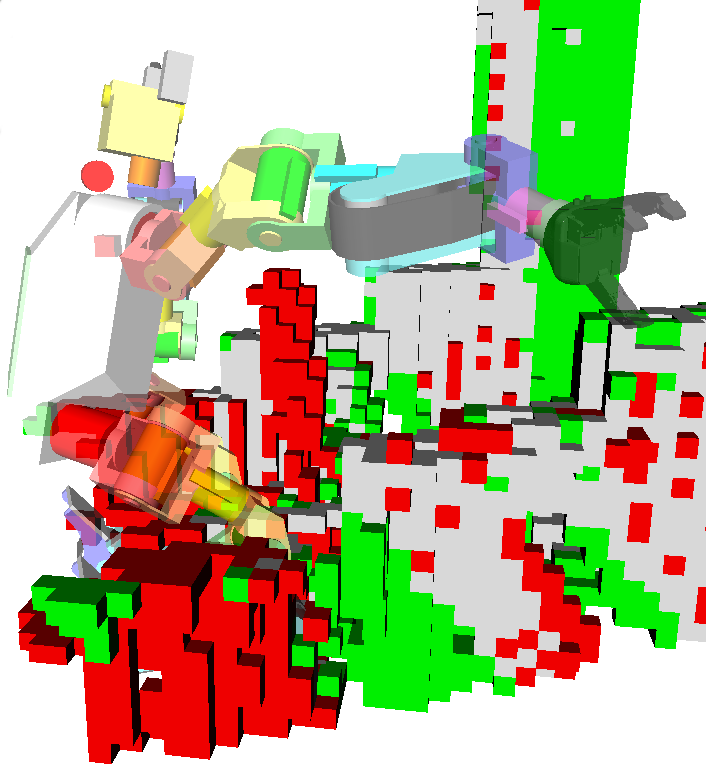
\includegraphics[width=0.56\columnwidth]{figs/chimp-voxels-delta.png}};

\node[draw,inner sep=3pt,fill=white,fill opacity=0.9,align=center]
  (debrislab) at (-0.7,3.5) {Debris object\\removed};
\node[circle,inner sep=2,draw,fill=white] (debris) at (2.0,2.9) {};
\draw[draw=black, double=white, double distance=1pt, line width=1pt]
  (debrislab.east) -- (debris);
  
\node[draw,inner sep=3pt,fill=white,fill opacity=0.9,align=center]
  (debrislab) at (5.8,5.2) {Additional\\voxels seen};
\node[circle,inner sep=2,draw,fill=white] (debris) at (4.2,5.0) {};
\draw[draw=black, double=white, double distance=1pt, line width=1pt]
  (debrislab.west) -- (debris);
  
\end{tikzpicture}
\caption{A disaster response robot maintains a
  dynamic unstructured environment model
  using coarse voxels
  (scene data from a debris-clearing task at a
  recent disaster response competition).
  Since the last planning query,
  voxels have been added (green) and removed (red).}
\label{fig:chimp-voxels-delta}
\end{subfigure}

\vspace{0.1in}

\begin{subfigure}[b]{\linewidth}
\centering
\documentclass{standalone}
\usepackage{tikz}
\usetikzlibrary{calc}
\begin{document}
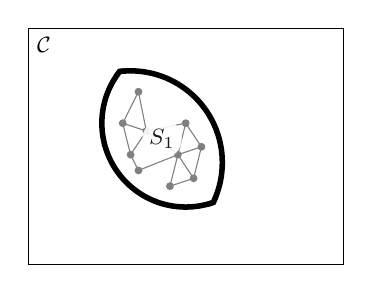
\begin{tikzpicture}

\tikzstyle{every node}=[font=\footnotesize]

\draw (0,0) rectangle (4.0,3.0);

\coordinate (a) at (2.0,1.8);
\coordinate (b) at (1.3,1.3);

\def\circlea{(a) circle (1.1)}
\def\circleb{(b) circle (1.2)}

% AnB
\begin{scope}
   \clip \circlea;
   \clip \circleb;
   \draw[line width=4pt] \circlea;
   \draw[line width=4pt] \circleb;
\end{scope}

% roadmap
\coordinate (v01) at ($ (a) + ( 0.0, 0.0) $);
\coordinate (v02) at ($ (a) + (-0.1,-0.4) $);
\coordinate (v03) at ($ (a) + ( 0.1,-0.7) $);
\coordinate (v04) at ($ (a) + (-0.2,-0.8) $);
\coordinate (v05) at ($ (a) + (-0.6,-0.6) $);
\coordinate (v06) at ($ (a) + (-0.7,-0.4) $);
\coordinate (v07) at ($ (a) + (-0.5,-0.1) $);
\coordinate (v08) at ($ (a) + ( 0.2,-0.3) $);
\coordinate (v09) at ($ (a) + (-0.8, 0.0) $);
\coordinate (v10) at ($ (a) + (-0.6, 0.4) $);
\node[circle,fill=black!50,inner sep=1.0] at (v01) {};
\node[circle,fill=black!50,inner sep=1.0] at (v02) {};
\node[circle,fill=black!50,inner sep=1.0] at (v03) {};
\node[circle,fill=black!50,inner sep=1.0] at (v04) {};
\node[circle,fill=black!50,inner sep=1.0] at (v05) {};
\node[circle,fill=black!50,inner sep=1.0] at (v06) {};
\node[circle,fill=black!50,inner sep=1.0] at (v07) {};
\node[circle,fill=black!50,inner sep=1.0] at (v08) {};
\node[circle,fill=black!50,inner sep=1.0] at (v09) {};
\node[circle,fill=black!50,inner sep=1.0] at (v10) {};
\draw[color=black!50]
   (v01) -- (v02) -- (v03) -- (v04) -- (v02) -- (v05) -- (v06)
   -- (v07) -- (v02) -- (v08);
\draw[color=black!50] (v03) -- (v08) -- (v01) -- (v07);
\draw[color=black!50] (v06) -- (v09) -- (v07) -- (v10) -- (v09);

\node at (0.2,2.8) {$\mathcal{C}$};

\node[circle,inner sep=1pt,fill=white,fill opacity=0.9]
  at (1.7,1.6) {$S_1$};

\end{tikzpicture}%
\end{document}

\documentclass{standalone}
\usepackage{tikz}
\usetikzlibrary{calc}
\begin{document}
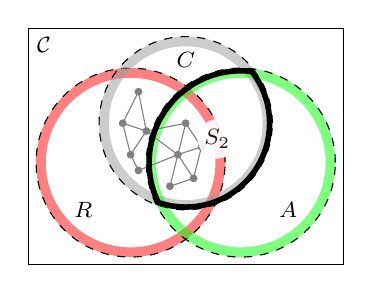
\begin{tikzpicture}

\tikzstyle{every node}=[font=\footnotesize]

\draw (0,0) rectangle (4.0,3.0);

\coordinate (a) at (2.0,1.8);
\coordinate (b) at (1.3,1.3);
\coordinate (c) at (2.7,1.3);

\def\circlea{(a) circle (1.1)}
\def\circleb{(b) circle (1.2)}
\def\circlec{(c) circle (1.2)}

% underlying sets
\begin{scope}
   \clip \circleb;
   \draw[color=red!50,line width=7pt] \circleb;
\end{scope}
\draw[dashed] \circleb;

\begin{scope}
   \clip \circlea;
   \draw[color=black!40,opacity=0.5,line width=7pt] \circlea;
\end{scope}
\draw[dashed] \circlea;

\begin{scope}
   \clip \circlec;
   \draw[color=green,opacity=0.5,line width=7pt] \circlec;
\end{scope}
\draw[dashed] \circlec;

% roadmap
\coordinate (v01) at ($ (a) + ( 0.0, 0.0) $);
\coordinate (v02) at ($ (a) + (-0.1,-0.4) $);
\coordinate (v03) at ($ (a) + ( 0.1,-0.7) $);
\coordinate (v04) at ($ (a) + (-0.2,-0.8) $);
\coordinate (v05) at ($ (a) + (-0.6,-0.6) $);
\coordinate (v06) at ($ (a) + (-0.7,-0.4) $);
\coordinate (v07) at ($ (a) + (-0.5,-0.1) $);
\coordinate (v08) at ($ (a) + ( 0.2,-0.3) $);
\coordinate (v09) at ($ (a) + (-0.8, 0.0) $);
\coordinate (v10) at ($ (a) + (-0.6, 0.4) $);
\node[circle,fill=black!50,inner sep=1.0] at (v01) {};
\node[circle,fill=black!50,inner sep=1.0] at (v02) {};
\node[circle,fill=black!50,inner sep=1.0] at (v03) {};
\node[circle,fill=black!50,inner sep=1.0] at (v04) {};
\node[circle,fill=black!50,inner sep=1.0] at (v05) {};
\node[circle,fill=black!50,inner sep=1.0] at (v06) {};
\node[circle,fill=black!50,inner sep=1.0] at (v07) {};
\node[circle,fill=black!50,inner sep=1.0] at (v08) {};
\node[circle,fill=black!50,inner sep=1.0] at (v09) {};
\node[circle,fill=black!50,inner sep=1.0] at (v10) {};
\draw[color=black!50]
   (v01) -- (v02) -- (v03) -- (v04) -- (v02) -- (v05) -- (v06)
   -- (v07) -- (v02) -- (v08);
\draw[color=black!50] (v03) -- (v08) -- (v01) -- (v07);
\draw[color=black!50] (v06) -- (v09) -- (v07) -- (v10) -- (v09);

% AnC
\begin{scope}
   \clip \circlea;
   \clip \circlec;
   \draw[line width=4pt] \circlea;
   \draw[line width=4pt] \circlec;
\end{scope}

\node at (0.2,2.8) {$\mathcal{C}$};
\node at ($ (a) + (0,0.8) $) {$C$};
\node at ($ (b) + (-0.6,-0.6) $) {$R$};
\node at ($ (c) + ( 0.6,-0.6) $) {$A$};

\node[circle,inner sep=1pt,fill=white,fill opacity=0.9]
  at (2.4,1.6) {$S_2$};

\end{tikzpicture}%
\end{document}

\caption{
  $\mathcal{C}$-subsets and relations
  can be added retroactively.
  Here, the graph for an initial query is checked w.r.t $X_1$.
  After environment changes,
  $X_1$ is redefined in terms of the $\mathcal{C}$-subsets
  derived from the set of common, added, and removed elements,
  allowing for reuse on a query in $X_2$.
  Here,
  the planner need only check existing path segments
  against added voxels in order to reuse them for the current query.}
\label{fig:retroactive}
\end{subfigure}

\caption{
  Structured or unstructured dynamic environments
  can be represented as a multi-set problem
  (see Section~\ref{subsec:dynamic-environments}).}
\label{fig:dynamic-environments}
\end{figure}

The sensors on most articulated robots allow them to maintain
dynamic environment models to track changing collision geometry
(see Fig.~\ref{fig:chimp-voxels-delta}).
These models might be
structured (e.g. recognizing objects with known models)
or unstructured (e.g. occupancy models).
In both cases,
even in a changing world,
there are often areas that are fixed between planning queries.

Prior work (e.g. \cite{jaillet2004dynamicprm})
leverages this by imposing a dichotomy between
\emph{fixed} and \emph{moving} components of $\mathcal{C}$.
Our formulation extends this to an arbitrary number of such labels,
including ones defined retroactively (i.e. during planning;
see Fig.~\ref{fig:retroactive}).
By explicitly labeling such areas in workspace
(and leveraging the \emph{set containment} property
\cite{newmanbranicky1991cspacetransforms}),
we can represent this structure as a multi-set planning problem.

Special case of this is if objects are disappearing.

Relation to occupancy grid representations of workspace
(for deltas, conservative approxs, etc).

\subsection{Grasped Objects}
\label{subsec:grasped-objects}

One instance specific to manipulation problems is the handling of
grasped objects.
For example, 
consider a manipulator which grasps a geometric object.
This affects the set of collision-free configurations
across a large section of $\mathcal{C}$
relative to the old set of valid configurations $X_{old}$.
However,
the resulting $\mathcal{C}$-subset $X_{new}$
can be represented simply as
$X_{new} = X_{old} \cap G$,
with $G$ the set of robot configurations in which
the \emph{grasped object} (only)
is deemed free of collision with the robot and environment.
This structure is discussed in the context of the
\emph{conditional reachability graph},
part of the \textsc{FFRob} heuristic framework
\cite{garrett2014ffrob}.

For example,
consider the manipulation problem in
Figure~\ref{fig:testherb-problem}.
The robot must find a path which moves its arm to grasp the cup.
After the cup is grasped,
the robot can reuse any edge in the existing roadmap
but simply checking the grasped cup
against the remainder of the environment.
This structure,
together with the approach to dynamic environments,
are included together in the experimental results
(Section~\ref{subsec:herb-experiment}).

\begin{figure}
\centering
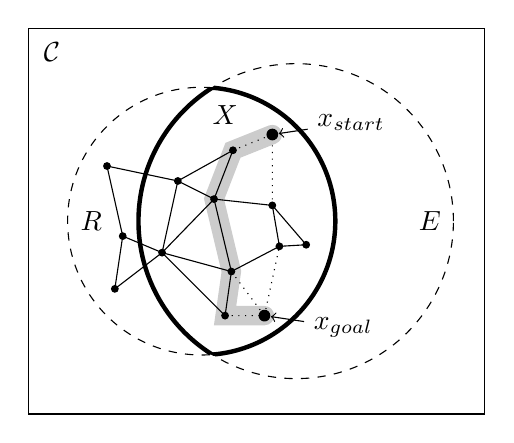
\begin{tikzpicture}

\draw (0,0) rectangle (5.8,4.9);

\coordinate (r) at (2.2,2.45);
\coordinate (e) at (3.4,2.45);

\def\circler{(r) circle (1.7)}
\def\circlee{(e) circle (2.0)}

% XnY
\begin{scope}
   \clip \circler;
   %\fill[pattern=horizontal lines] \circley;
   \draw[ultra thick] \circlee;
\end{scope}
\begin{scope}
   \clip \circlee;
   \draw[ultra thick] \circler;
\end{scope}

\draw[dashed] \circler;
\draw[dashed] \circlee;

\node (clab) at (0.3,4.6) {$\mathcal{C}$};
\node (rlab) at ($ (r) + (-1.4,0) $) {$R$};
\node (elab) at ($ (e) + ( 1.7,0) $) {$E$};
\node (flab) at (2.5,3.8) {$X$};

\coordinate (v01) at ($ (r) + (-1.20, 0.70) $);
\coordinate (v02) at ($ (r) + (-1.10,-0.86) $);
\coordinate (v03) at ($ (r) + (-1.00,-0.19) $);
\coordinate (v04) at ($ (r) + (-0.50,-0.40) $);
\coordinate (v05) at ($ (r) + (-0.30, 0.51) $);
\coordinate (v07) at ($ (r) + ( 0.30,-1.20) $);
\coordinate (v08) at ($ (r) + ( 0.16, 0.28) $);
\coordinate (v09) at ($ (r) + ( 0.38,-0.64) $);
\coordinate (v06) at ($ (r) + ( 0.40, 0.90) $);
\coordinate (v10) at ($ (r) + ( 0.90, 0.20) $);
\coordinate (v11) at ($ (r) + ( 0.99,-0.32) $);
\coordinate (v12) at ($ (r) + ( 1.33,-0.30) $);
\coordinate (p1) at ($ (r) + (0.9, 1.1) $);
\coordinate (p2) at ($ (r) + (0.8,-1.2) $);

\draw[color=black!20,line width=7,line cap=round]
  (p2) -- (v07) -- (v09) -- (v08) -- (v06) -- (p1);

\node[circle,fill=black,inner sep=1.0] at (v01) {};
\node[circle,fill=black,inner sep=1.0] at (v02) {};
\node[circle,fill=black,inner sep=1.0] at (v03) {};
\node[circle,fill=black,inner sep=1.0] at (v04) {};
\node[circle,fill=black,inner sep=1.0] at (v05) {};
\node[circle,fill=black,inner sep=1.0] at (v07) {};
\node[circle,fill=black,inner sep=1.0] at (v08) {};
\node[circle,fill=black,inner sep=1.0] at (v09) {};
\node[circle,fill=black,inner sep=1.0] at (v06) {};
\node[circle,fill=black,inner sep=1.0] at (v10) {};
\node[circle,fill=black,inner sep=1.0] at (v11) {};
\node[circle,fill=black,inner sep=1.0] at (v12) {};

\draw (v01) -- (v03) -- (v02) -- (v04) -- (v03);
\draw (v01) -- (v05) -- (v04) -- (v07) -- (v09) -- (v04);
\draw (v04) -- (v08) -- (v05) -- (v06) -- (v08) -- (v10);
\draw (v08) -- (v09) -- (v11) -- (v10);
\draw (v11) -- (v12) -- (v10);

\node[circle,fill=black,inner sep=1.5] (p1node) at (p1) {};
\node[circle,fill=black,inner sep=1.5] (p2node) at (p2) {};
\draw[color=black,dotted] (v06) -- (p1) -- (v10);
\draw[color=black,dotted] (v07) -- (p2) -- (v09);
\draw[color=black,dotted] (p2) -- (v11);

\node (p1lab) at (4.1,3.7) {$x_{start}$};
\node (p2lab) at (4.0,1.1) {$x_{goal}$};
\draw[->] (p1lab) -- (p1node);
\draw[->] (p2lab) -- (p2node);

\end{tikzpicture}%

\caption{A roadmap is pre-computed in $R$,
  the subset of $\mathcal{C}$ consisting of configurations free
  of robot self-collision.
  Online, the planner must find a path that's also within $E$,
  the subset free of environment collision.
  When solving this query in $X = R \cap E$,
  the Multi-Set PRM automatically prefers potential paths with
  pre-computed edges (e.g. shown in grey)
  due to lower planning costs over alternatives with lower
  execution costs.}
\label{fig:self-collision-example}
\end{figure}

\subsection{Cached Self-Collision-Checked Roadmaps}
\label{subsec:cached-self-valid}

Self-collision checking is a potentially expensive component to
articulated motion planning;
in contrast to environment checking,
it is fundamentally quadratic in the number of moving links.
Further, pairs of links to be checked
tend to be relatively close to each other,
reducing the effeciveness of broad-phase approaches.

Leven and Hutchinson \cite{leven2000changing}
introduced the concept of a pre-cached roadmap consisting of
configurations and paths already known to be valid w.r.t.
self-collision.
As a type of invariant in $\mathcal{C}$,
this can be seen as a particular instance of multi-set planning.
See Fig.~\ref{fig:self-collision-example}.

\begin{figure}
\centering

\begin{subfigure}[t]{\linewidth}
\centering
\documentclass{standalone}
\usepackage{tikz}
\usetikzlibrary{positioning,shapes}
\begin{document}
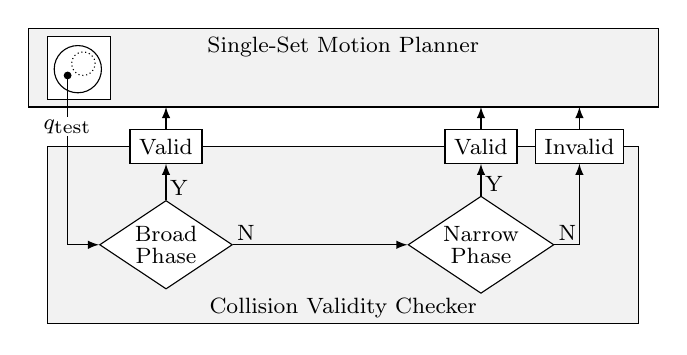
\begin{tikzpicture}

\tikzstyle{every node}=[font=\footnotesize]
\tikzset{>=latex} % arrow heads

\node[draw,rectangle,fill=black!5,
  inner sep=0,minimum width=8cm,minimum height=1.0cm]
  (boxmp) at (4,-0.5) {};
\node[above = -0.5cm of boxmp] {Single-Set Motion Planner};

% c-space depiction
\node[draw,fill=white,rectangle,
   minimum width=0.8cm,minimum height=0.8cm] at (0.65,-0.5) {};
\draw (0.63,-0.52) circle [radius=0.3cm];
\draw[densely dotted] (0.70,-0.45) circle [radius=0.15cm];
\node[circle,fill=black,inner sep=1.0] at (0.5,-0.6) {};

\node[draw,rectangle,fill=black!5,
  minimum width=7.5cm,minimum height=2.25cm]
  (boxcc) at (4,-2.625) {};
\node[below = -0.45cm of boxcc] {Collision Validity Checker};

\node[draw,fill=white,diamond,aspect=1.5,align=center,
  inner sep=1]
  (bp) at (1.75,-2.75) {Broad\\[-0.05cm]Phase};

\node[draw,fill=white,diamond,aspect=1.5,align=center,
  inner sep=1]
  (np) at (5.75,-2.75) {Narrow\\[-0.05cm]Phase};

\node[draw,fill=white,rectangle] (bv) at (1.75,-1.5) {Valid};

\node[draw,fill=white,rectangle] (nv) at (5.75,-1.5) {Valid};
\node[draw,fill=white,rectangle] (ni) at (7.0,-1.5) {Invalid};

\draw[->] (0.5,-0.6) -- (0.5,-2.75) -- (bp.west);
\draw[->] (bp.north) -- (bv.south);
\draw[->] (bv.north) -- (1.75,-1.0);
\draw[->] (bp.east) -- (np.west);
\draw[->] (np.north) -- (nv.south);
\draw[->] (nv.north) -- (5.75,-1.0);
\draw[->] (np.east) -- (7.0,-2.75) -- (ni.south);
\draw[->] (ni.north) -- (7.0,-1.0);

\node[rectangle,fill=white,inner sep=1] at (0.5,-1.25)
  {$q_{\mbox{\scriptsize test}}$};

\node[above right = -0.1cm of bp.north] {Y};
\node[above right = -0.1cm of bp.east] {N};
\node[above right = -0.1cm of np.north] {Y};
\node[above right = -0.1cm of np.east] {N};

%\draw[step=1,black!10,very thin] (0,-4) grid (8,0);

\end{tikzpicture}%
\end{document}

\caption{A single-set planner testing simply for membership in
  $\mathcal{C}_{free}$ treats a collision validity checker as a
  ``black box.''
  Internally,
  modern checkers first employ an inexpensive broad-phase check
  using a low-dimensional conservative representation
  to quickly identify non-colliding bodies before
  resorting to an expensive narrow-phase check.}
\end{subfigure}

\vspace{0.2in}

\begin{subfigure}[t]{\linewidth}
\centering
\documentclass{standalone}
\usepackage{tikz}
\usetikzlibrary{positioning,shapes}
\begin{document}
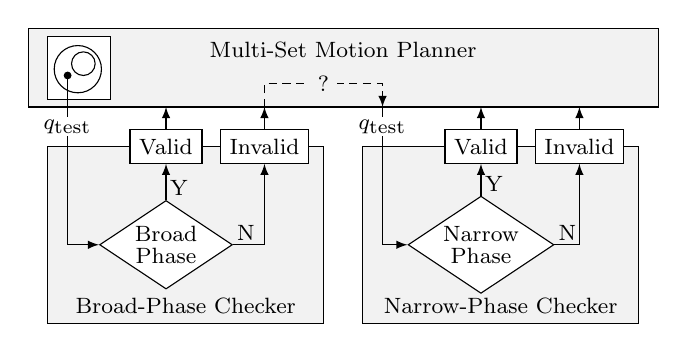
\begin{tikzpicture}

\tikzstyle{every node}=[font=\footnotesize]
\tikzset{>=latex} % arrow heads

\node[draw,rectangle,fill=black!5,
  inner sep=0,minimum width=8cm,minimum height=1.0cm]
  (boxmp) at (4,-0.5) {};
\node[above = -0.5cm of boxmp] {Multi-Set Motion Planner};

% c-space depiction
\node[draw,fill=white,rectangle,
   minimum width=0.8cm,minimum height=0.8cm] at (0.65,-0.5) {};
\draw (0.63,-0.52) circle [radius=0.3cm];
\draw (0.70,-0.45) circle [radius=0.15cm];
\node[circle,fill=black,inner sep=1.0] at (0.5,-0.6) {};

\node[draw,rectangle,fill=black!5,
  minimum width=3.5cm,minimum height=2.25cm]
  (boxcc) at (2,-2.625) {};
\node[below = -0.45cm of boxcc] {Broad-Phase Checker};

\node[draw,rectangle,fill=black!5,
  minimum width=3.5cm,minimum height=2.25cm]
  (boxcc) at (6,-2.625) {};
\node[below = -0.45cm of boxcc] {Narrow-Phase Checker};

\node[draw,fill=white,diamond,aspect=1.5,align=center,
  inner sep=1]
  (bp) at (1.75,-2.75) {Broad\\[-0.05cm]Phase};

\node[draw,fill=white,diamond,aspect=1.5,align=center,
  inner sep=1]
  (np) at (5.75,-2.75) {Narrow\\[-0.05cm]Phase};

\node[draw,fill=white,rectangle] (bv) at (1.75,-1.5) {Valid};
\node[draw,fill=white,rectangle] (bi) at (3.0,-1.5) {Invalid};

\node[draw,fill=white,rectangle] (nv) at (5.75,-1.5) {Valid};
\node[draw,fill=white,rectangle] (ni) at (7.0,-1.5) {Invalid};

\draw[->] (0.5,-0.6) -- (0.5,-2.75) -- (bp.west);
\draw[->] (bp.north) -- (bv.south);
\draw[->] (bv.north) -- (1.75,-1.0);
\draw[->] (bp.east) -- (3.0,-2.75) -- (bi.south);
\draw[->] (bi.north) -- (3.0,-1.0);

\draw[densely dashed] (3.0,-1.0) -- (3.0,-0.7) -- (3.6,-0.7);
\draw[->,densely dashed] (3.9,-0.7) -- (4.5,-0.7) -- (4.5,-1.0);

\draw[->] (4.5,-1.0) -- (4.5,-2.75) -- (np.west);
\draw[->] (np.north) -- (nv.south);
\draw[->] (nv.north) -- (5.75,-1.0);
\draw[->] (np.east) -- (7.0,-2.75) -- (ni.south);
\draw[->] (ni.north) -- (7.0,-1.0);

\node[rectangle,fill=black!5,inner sep=3] at (3.75,-0.7) {?};

\node[rectangle,fill=white,inner sep=1] at (0.5,-1.25)
  {$q_{\mbox{\scriptsize test}}$};
\node[rectangle,fill=white,inner sep=1] at (4.5,-1.25)
  {$q_{\mbox{\scriptsize test}}$};

\node[above right = -0.1cm of bp.north] {Y};
\node[above right = -0.1cm of bp.east] {N};
\node[above right = -0.1cm of np.north] {Y};
\node[above right = -0.1cm of np.east] {N};

%\draw[step=1,black!10,very thin] (0,-4) grid (8,0);

\end{tikzpicture}%
\end{document}

\caption{A multi-set planner can explicitly reason about the
  conservative nature of the broad-phase check.
  This allows it to defer some narrow phase checks
  (often indefinitely)
  and instead prefer paths that require fewer expensive checks.}
\end{subfigure}

\caption{Collision validity checking is a commonly used
  indicator function.
  The multi-set formulation allows an intelligent planner to
  reach inside the checker's ``black box'' and reduce the number
  of costly narrow-phase checks.
  Resulting paths tend to be cheaper to compute and
  stay further from obstacles.}
\label{fig:broad-phase}
\end{figure}

\subsection{Integration with Broad-Phase Collision Checking}
\label{subsec:broad-phase}

\begin{figure}
\centering

\begin{subfigure}[t]{0.45\linewidth}
\centering
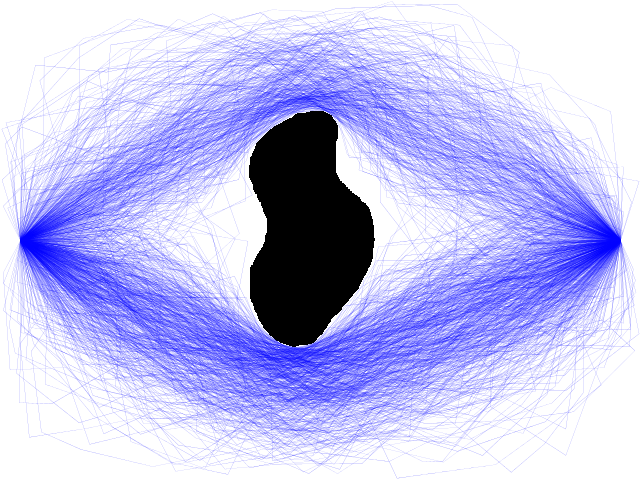
\includegraphics[width=\columnwidth]{figs/paths-lambda0-norel.png}
\caption{
  $\lambda=0$, no broad phase.\\
  Median planning cost: 6650}
\end{subfigure}
\begin{subfigure}[t]{0.45\linewidth}
\centering
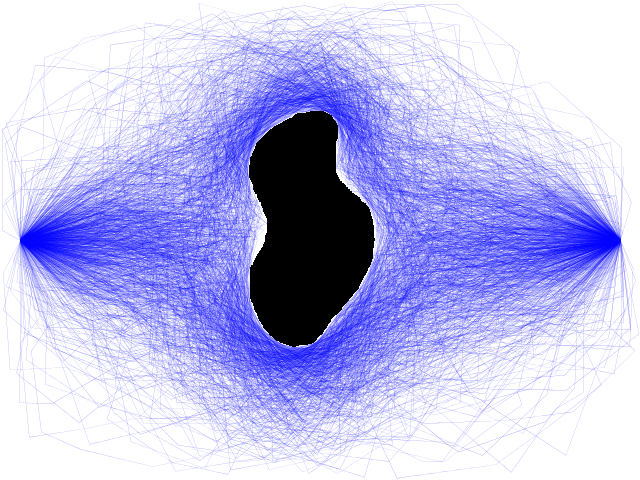
\includegraphics[width=\columnwidth]{figs/paths-lambda1-norel.png}
\caption{
  $\lambda=1$, no broad phase.\\
  Median planning cost: 4530}
\end{subfigure}

\begin{subfigure}[t]{0.45\linewidth}
\centering
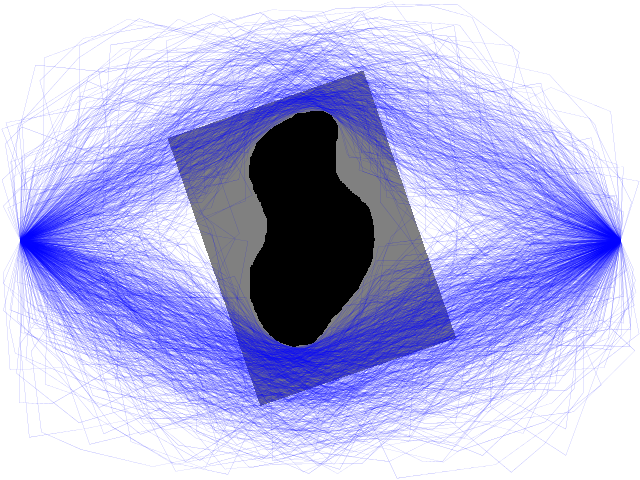
\includegraphics[width=\columnwidth]{figs/paths-lambda0-wrel.png}
\caption{
  $\lambda=0$, with broad phase.\\
  Median planning cost: 2122}
\end{subfigure}
\begin{subfigure}[t]{0.45\linewidth}
\centering
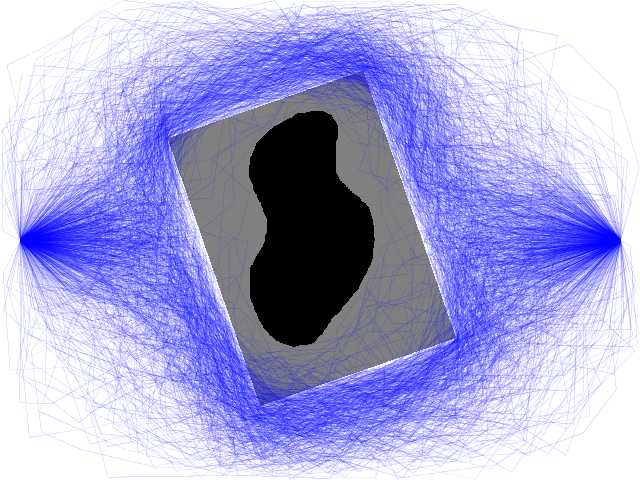
\includegraphics[width=\columnwidth]{figs/paths-lambda1-wrel.png}
\caption{
  $\lambda=1$, with broad phase.\\
  Median planning cost: 737}
\end{subfigure}

\caption{A simple 2D example of the Multi-Set PRM using
  a broad-phase check.
  Checking for collision with the grey box is 10x less expensive
  than with the actual black obstacle.
  \cdnote{I need to talk about this in the text.}}
\label{fig:broad-phase-2d}
\end{figure}

The multi-set formulation also enables motion planners to
reason directly about different robot or environment models.
For example, consider two geometric robot models,
one with high quality (e.g. from a CAD program),
and one hand-tuned ``padded'' model consisting of 
a small number of simple conservative bounding volumes.
The $\mathcal{C}$-subsets derived from these models,
are related by $R_{padded} \subseteq R_{CAD}$.
Collision checkers currently use a similar approach internally
to speed up collision checks (see Fig.~\ref{fig:broad-phase}.
and Fig~\ref{fig:broad-phase-2d}).

\subsection{Conservative Bounding Volumes for Different Grasps}

\subsection{Conservative Bounding Volumes for Hypothesized Objects}

There's a sweet ICRA paper here.

\subsection{Dual Arm Stuff}

I think this is related.

Check right arm against gian left side box, etc.

\subsection{Dimensionality Reduction}

The Handey \cite{lozanoperez1987handey} robot
assumed a box that contained the wrist links at a range of DOF values.

\section{Other Stuff}

Potential research question: learn cost model over time.


\newpage
\chapter{Applying Greedy PRM to Multi-Set: the Multi-Set Greedy PRM}
\label{chap:multi-set-prm}

\begin{itemize}
\item GreedyPRM and multi-set are complementary
\item Apply greeydprm to multi-set problem
\item one planner that learns, can answer arbitrary queries
   in multiple related spaces faster and faster
\end{itemize}

\section{From RSS Intro}

This computational burden is especially troublesome
in time-sensitive human-scale manipulation tasks
(e.g. from household or disaster response domains).
The costs incurred by the planner
(computation time / electrical energy)
and the robot's motor controllers
(execution time / mechanical energy)
tend to be of comparable magnitude in such domains.
As a result,
we'd like an approach which can reason about both
planning \emph{and} execution costs,
striving for a balance between feasibility and optimality.

Our second key insight
is to apply the principle of best-first search over roadmaps
using an objective which explicitly considers both planning and
execution costs.
The result is the Multi-Set PRM (Section~\ref{chap:multi-set-prm}).
This approach allows the planner to exploit the multi-set structure
inherent in these problems.
%We show the relation of this approach to inflated heuristics
%when applied to traditional graph search over implicit graphs.

\section{Related Work}

Also, there are incremental E-graphs \cite{phillips2013anytimeegraphs}
that we should relate the planner to and compare with.

\section{Implementation Details}

\subsection{Calculating the Optimistic Path Cost}
\label{subsec:alg-opt-path-cost}

The execution cost component is given by $f_e[x(t)]$
as defined in the cost model $\mathcal{M}$
(Section~\ref{subsec:cost-model}).
The optimistic estimate of the remaining planning cost for the path
is computed by determining the cost of the optimistic plan for each
edge using the \textsc{OptEdgePlan} function
(Section~\ref{subsec:alg-opt-edge-plan}).

\begin{algorithm}
\caption{Calculating the Optimistic Edge Plan}
\label{alg:opt-edge-plan}
\begin{algorithmic}[1]
\Function {$\mbox{\textsc{OptEdgePlan}}$}{$e$}
   \State $(S_{best}, b_{best}, c_{best})
      \leftarrow (\mbox{\textbf{nil}}, \mbox{\textbf{nil}}, \infty)$
   \ForAll {$S \in \mathcal{P}(\mathcal{S})$}
         \label{line:power-set}
      \State $c = \sum_{X \in S} f_X[e]$
      \ForAll {$b \mbox{ \textbf{s.t.} }
            b : S \rightarrow \{\mbox{True},\mbox{False}\}$}
            \label{line:all-binary-functions}
         \State $\arraycolsep=2pt
            P_{new} =
            \left\{\left.\left( \begin{array}{rl}
            \mathbf{1}_X & \mbox{if } b(X) \\
            \lnot \mathbf{1}_X & \mbox{otherwise} \\
            \end{array} \right)
            \right|
            X \in S
            \right\}$
         \If {$P_{rels} \cup e.P \cup P_{new}
               \Rightarrow \mathbf{1}_{X_g}$ is valid}
            \If {$c < c_{best}$}
               \State $(S_{best}, b_{best}, c_{best})
                  \leftarrow (S, b, c)$
            \EndIf
         \EndIf
      \EndFor
   \EndFor
   \State \Return $(S_{best}, b_{best}, c_{best})$
\EndFunction
\end{algorithmic}
\end{algorithm}

\subsection{Calculating the Optimistic Edge Plan}
\label{subsec:alg-opt-edge-plan}

The \textsc{OptEdgePlan} function (Alg.~\ref{alg:opt-edge-plan})
performs the core reasoning which exploits the relations in
the multi-set problem.
Before discussing its implementation,
we first briefly discuss the propositional logic approach
used to reason about the state of each edge.

The planner represents the list of set relations $\mathcal{R}$
(Section~\ref{subsec:problem-definition})
specified in the multi-set problem formulation
as a set of \emph{logical propositions} $P_{rels}$
which are considered globally applicable.
For example,
the proposition $\mathbf{1}_A \Rightarrow \mathbf{1}_B$
follows from the relation $A \subseteq B$
(see Fig.~\ref{fig:relations}).
In addition,
each edge $e$ in the roadmap is augmented with an initially empty
set $e.P$ containing all additional edge-specific propositions
known to be true as a result of any indicator functions evaluated
over that edge.
For example,
if planner evaluated the indicator $\mathbf{1}_B[e]$
and it returned False,
the proposition $\lnot\mathbf{1}_B$ would be added to $e.P$.
Together, such sets of propositions can be used as \emph{premises}
as part of an \emph{argument} to demonstrate a \emph{conclusion};
a logical solver can then be used validate or invalidate the argument.
For example, an argument with these premises and conclusion
$\{ (\mathbf{1}_A \Rightarrow \mathbf{1}_B), (\lnot\mathbf{1}_B) \}
\Rightarrow (\lnot\mathbf{1}_A)$
can be shown to be valid.

The \textsc{OptEdgePlan} function (Alg.~\ref{alg:opt-edge-plan})
is tasked with computing
the optimistically optimal set of indicator evaluations to perform
for the edge in order to validate its membership in the query
$\mathcal{C}$-subset $X_g$.
The function returns three elements:
(a) the set of $\mathcal{C}$-subsets $S \subseteq \mathcal{S}$
whose indicators are to be evaluated,
(b) a binary function $b$
which provides the desired indicator result for each evaluation,
and (c) the total evaluation cost $c$
given by the cost model $\mathcal{M}$'s $f_X[\cdot]$ functionals
(Section~\ref{subsec:cost-model}).

The function proceeds by considering all combinations of
available $\mathcal{C}$-subset indicators $S$ (line~\ref{line:power-set}).
For each set of evaluations,
we compute the planning cost $c$ which would be required.
We then consider all possible outcomes for each indicator
by iterating over all functions $b$ mapping
from $\mathcal{C}$-subset $X$ to binary values
(line~\ref{line:all-binary-functions}).
For each potential outcome $b$,
we form the set of additional propositions $P_{new}$,
and then use a logic solver to determine whether the aggregate
premises imply membership in the query $\mathcal{C}$-subset $X_g$.
If so (and the required cost is the best so far),
we save and return it.

\subsection{Home Robot Manipulation Task}
\label{subsec:herb-experiment}

\begin{figure*}
\begin{widepage}
\centering

\begin{subfigure}[t]{0.185\linewidth}
\centering
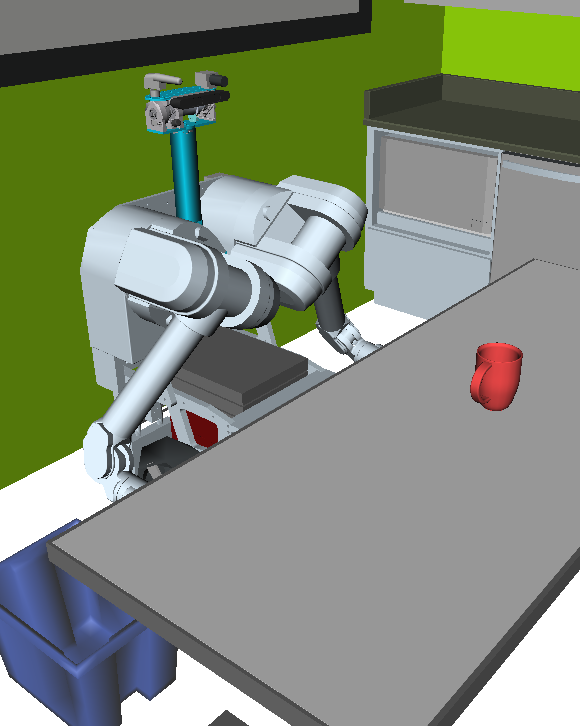
\includegraphics[width=\columnwidth]{figs/testherb-a.png}
\caption{Starting Configuration}
\end{subfigure}
\begin{subfigure}[t]{0.185\linewidth}
\centering
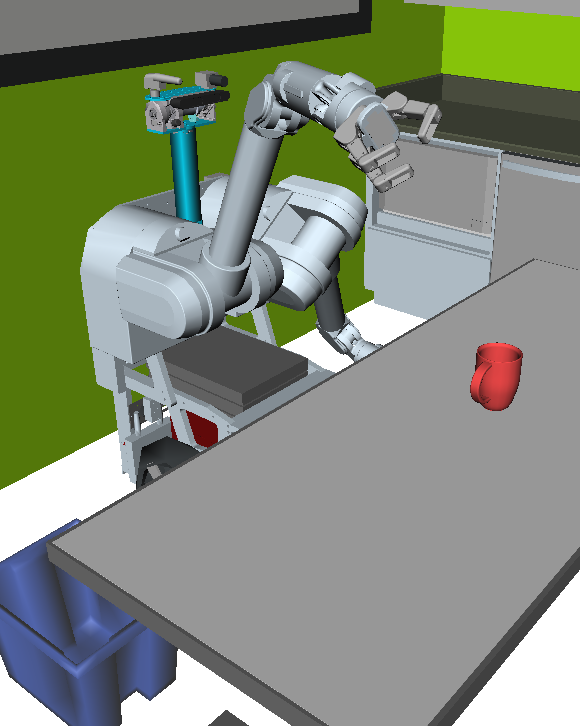
\includegraphics[width=\columnwidth]{figs/testherb-b.png}
\caption{Step 1, in $X_1$}
\end{subfigure}
\begin{subfigure}[t]{0.185\linewidth}
\centering
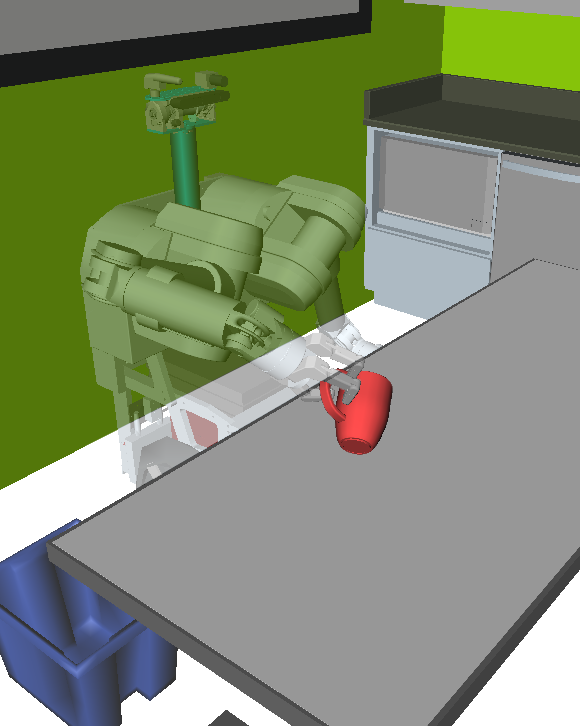
\includegraphics[width=\columnwidth]{figs/testherb-c.png}
\caption{Step 2, in $X_2$}
\end{subfigure}
\begin{subfigure}[t]{0.185\linewidth}
\centering
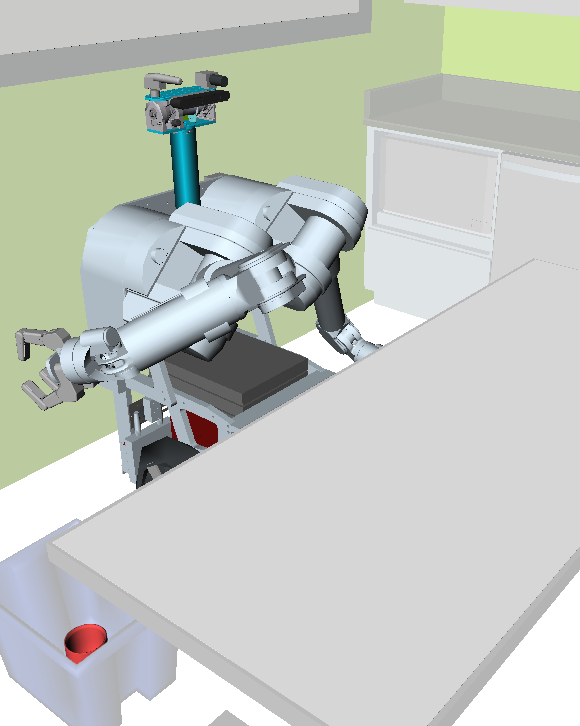
\includegraphics[width=\columnwidth]{figs/testherb-d.png}
\caption{Step 3, in $X_3$}
\end{subfigure}
\begin{subfigure}[t]{0.185\linewidth}
\centering
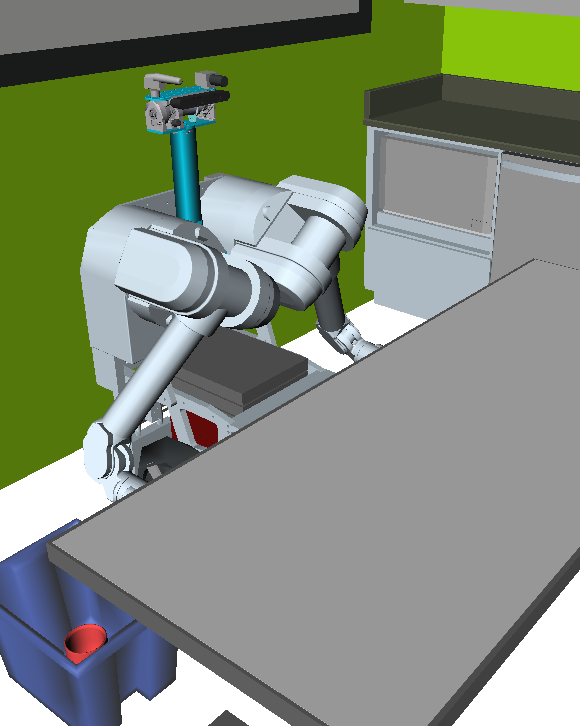
\includegraphics[width=\columnwidth]{figs/testherb-e.png}
\caption{Ending Configuration.}
\end{subfigure}

\caption{
  A home robot performing a three-step manipulation task.
  It must move from its home configuration
  to grasp the cup,
  transfer it to a drop location above the bin,
  and return home.
  Experimental results for the Multi-Set PRM
  are shown in Table~\ref{tab:testherb}}
\label{fig:testherb-problem}
\end{widepage}
\end{figure*}

\begin{table*}
\begin{widepage}
\centering
\footnotesize
\setlength{\tabcolsep}{3pt}
\renewcommand{\arraystretch}{1.3}
\begin{tabular}{|cc|r@{ }lr@{ }lr@{ }lr@{ }l|r@{ }lr@{ }lr@{ }lr@{ }l|r@{ }lr@{ }lr@{ }lr@{ }l|}
\toprule
\multirow{2}{*}{Relations} & \multirow{2}{*}{Cost}
  & \multicolumn{8}{c|}{$\lambda = 0$}
  & \multicolumn{8}{c|}{$\lambda = 0.5$}
  & \multicolumn{8}{c|}{$\lambda = 1$}
\\
  &
  & Step & 1 & Step & 2 & Step & 3 & \multicolumn{2}{c|}{Total}
  & Step & 1 & Step & 2 & Step & 3 & \multicolumn{2}{c|}{Total}
  & Step & 1 & Step & 2 & Step & 3 & \multicolumn{2}{c|}{Total}
\\ \midrule
\multirow{2}{*}{None} & Plan
  &  6.16&s &  3.72&s &  2.38&s & 12.25&s
  &  5.52&s &  2.89&s &  2.12&s & 10.53&s
  &  3.39&s &  2.25&s &  2.12&s &  7.76&s
\\
  & Exec
  & 14.22&rad &  8.51&rad &  4.23&rad & 26.97&rad
  & 15.07&rad & 10.60&rad &  4.23&rad & 29.89&rad
  & 15.07&rad & 10.60&rad &  4.23&rad & 29.89&rad
\\ [1ex]
Inter-Step & Plan
  &  6.40&s &  2.33&s &  0.86&s &  9.59&s
  &  5.40&s &  1.55&s &  0.91&s &  7.86&s
  &  3.38&s &  0.91&s &  0.30&s &  4.59&s
\\
(Sec.~\ref{subsec:dynamic-environments},~\ref{subsec:grasped-objects})
  & Exec
  & 14.22&rad &  8.51&rad &  4.23&rad & 26.97&rad
  & 15.07&rad & 12.21&rad &  4.23&rad & 31.51&rad
  & 15.07&rad & 12.21&rad &  7.11&rad & 34.40&rad
\\ [1ex]
Self-Checked & Plan*
  &  3.54&s &  2.23&s &  1.17&s & 6.94&s
  &  2.99&s &  1.77&s &  1.16&s & 5.92&s
  &  1.47&s &  1.22&s &  1.16&s & 3.85&s
\\
(Sec.~\ref{subsec:cached-self-valid}) & Exec
  & 14.22&rad &  8.51&rad &  4.23&rad & 26.96&rad
  & 14.22&rad & 10.06&rad &  4.23&rad & 28.51&rad
  & 14.22&rad & 10.60&rad &  4.23&rad & 29.05&rad
\\ [1ex]
\multirow{2}{*}{Both} & Plan*
  &  3.25&s &  1.79&s &  0.90&s & 5.94&s
  &  2.88&s &  1.55&s &  0.92&s & 5.35&s
  &  1.47&s &  1.88&s &  0.31&s & 3.66&s
\\
  & Exec
  & 14.22&rad &  8.51&rad &  4.23&rad & 26.96&rad
  & 14.22&rad &  8.51&rad &  4.23&rad & 26.96&rad
  & 14.22&rad &  9.64&rad &  6.36&rad & 30.22&rad
\\ 
\bottomrule
\end{tabular}
\caption{Home robot manipulation task results.
  The entry with no relations and $\lambda=0$ is equivalent
  to the LazyPRM.}
\label{tab:testherb}
\end{widepage}
\end{table*}

We tested the Multi-Set PRM on the manipulation task
described in Fig.~\ref{fig:testherb-problem}.
We used the $r$-disk PRM construction rule with $r=2.0$ rad,
and a batch size of $N=1000$.
Planning times are measured on a Lenovo T430 laptop.
The planner was asked to solve each of the steps of the plan
sequentially.

We varied
(a) the planning vs. execution parameter $\lambda$
(see Section~\ref{subsec:alg-opt-path-cost}), and
(b) the subset relations provided to the planner
as described in Sections
\ref{subsec:dynamic-environments},
\ref{subsec:grasped-objects},
and \ref{subsec:cached-self-valid}.
We measured the time required for planning (s)
and the length of the resulting solution resulting path (rad)
for each step of the task.

Note that the Multi-Set PRM,
with no relations specified and $\lambda=0$
reduces to the Lazy PRM.
As expected,
increasing $\lambda$ resulted in decreased planning times
but yielded longer paths.
Including more $\mathcal{C}$-subset relations
also significantly reduced planning times,
and had little effect on path lengths on this problem.
Note that the planning time results when using
the cached self-collision-checked roadmap, denoted by (*),
do not include the pre-computation time.

Note that including inter-step relations drastically
reduces planning times for subsequent steps.
We expect this trend would continue as more steps are included.
Also, note that when $\lambda=0$,
path length is unchanged as the number of set relations is
changed
-- this is because the paths that are selected for evaluation
by the algorithm are a function only of their (constant) lengths.

\section{Other Experiments to Run}

\begin{itemize}
\item with/without inter-step relations
\item with/without padding
\item with/without self-checked cache
\item with/without relations for changing worlds
\item with/without conservative boxes for grabbed objects
\item constraints:
   \begin{itemize}
   \item handle with separate planner
   \item handle with relaxed constraint, followed by local optimizer
   \end{itemize}
\item run optimizer on paths occasionally and/or before executing
\end{itemize}


\newpage
\chapter{Conclusion}

meta-graph [future work: probabalistic models]


\newpage
\chapter[Summary of Proposed Work]{Summary of\\Proposed Work}

\section{Open-Source Software}

\begin{itemize}
\item Release implementation of checkmask PRM (OMPL)
\item Release implementation of multi-set decomposer (OpenRAVE+OMPL)
\item Re-release orcdchomp with permissive license?
\end{itemize}

\section{Timeline}

See Table~\ref{table:timeline} for the timeline.

\begin{table}
\centering
\begin{tabular}{lll}
\hline
Topic & Sec. & Deadline \\
\hline
Greedy PRM, Multi-Set Planning & & January 2015 (RSS) (completed) \\
Proposal & & February 2015 \\
The Greedy PRM: Optimizing Total Task Cost & & March 2015 (IROS) \\
DRC Integration & & April-May 2015 \\
Multi-Set Planning at the DRC & & June 2015 (Humanoids) \\
Bored Robots: Hypothesized Conservative Volumes & & October 2015 (ICRA) \\
Writing & & November 2015 \\
Defence & & December 2015 \\
\hline
\end{tabular}
\caption{Proposed Timeline}
\label{table:timeline}
\end{table}


{\small
\bibliographystyle{abbrv}
\bibliography{pr-refs}
}

\appendix
\chapter{Graph Search Proofs}
\label{appendix:gs-proofs}

This appendix presents some proofs relating the path-centric treatment
of graph search from Chapter~\ref{chap:inflate}
to traditional algorithms (e.g. A$^*$).

\begin{invariant}
The optimistically optimal path $path^* = A_s(G)$ can always be
segmented into
(a) a first sequence comprised of zero or more evaluated edges,
followed by
(b) a second sequence comprised of zero or more non-evaluated edges.
\label{inv:path-segmentation}
\end{invariant}

\begin{theorem}
Invariant~\ref{inv:path-segmentation} holds throughout the course of
$E_s$ [forward] (Algorithm~WHAT?).
\label{thm:seg-fwd}
\end{theorem}

\begin{proof}
At the first iteration, with no edges evaluated,
$path^*$ will contain only non-evaluated edges,
and the invariant trivially holds.

Consider the case where the invariant newly does not hold for $path^*$.
In this case, there exists at least one triple of adjacent vertices
on the path $v_a, v_b, v_c$
such that the edge $(v_a, v_b)$ is un-evaluated,
while the edge $(v_b, v_c)$ has been evaluated.
Due to our invariant,
there must have been some previous iteration which returned a
$path'^*$ which contained the triple
$v'_a, v_b, v_c$ for some other $v'_a$,
with $(v'_a, v_b)$ evaluated.
Therefore, the shortest distance to $v_b$ must known (and can be
reached through $v'_a$),
and any subsequent optimistic-optimal path through $v_b$
must consist of only evaluated segments until $v_b$
(due to the way $A_s$ breaks ties).
But our current $path^*$'s segment $(v_a, v_b)$ is un-evaluated!
This contradiction shows that the invariant must hold throughout the
algorithm.
\end{proof}

\end{document}
